% **************************************************
% Document Class Definition
% **************************************************
\documentclass[%
    paper=A4,               % paper size --> A4 is default in Germany
    twoside=true,           % onesite or twoside printing
    openright,              % doublepage cleaning ends up right sidesirthe
    parskip=half,           % spacing value / method for paragraphs
    chapterprefix=true,     % prefix for chapter marks
    11pt,                   % font size
    headings=normal,        % size of headings
    bibliography=totoc,     % include bib in toc
    listof=totoc,           % include listof entries in toc
    titlepage=on,           % own page for each title page
    captions=tableabove,    % display table captions above the float env
    chapterprefix=false,    % do not display a prefix for chapters
    appendixprefix=false,    % but display a prefix for appendix chapter
    draft=false,            % value for draft version
]{scrreprt}%


% **************************************************
% Setup YOUR thesis document in this file !
% **************************************************
% !TEX root = my-thesis.tex


% **************************************************
% Files' Character Encoding
% **************************************************
\PassOptionsToPackage{utf8}{inputenc}
\usepackage{inputenc}


% **************************************************
% Information and Commands for Reuse
% **************************************************
\newcommand{\thesisTitle}{Sustaining glacial-fed irrigation networks with artificial ice reservoirs}
\newcommand{\thesisName}{Suryanarayanan Balasubramanian}
\newcommand{\thesisSubject}{Artificial Ice Reservoirs}
\newcommand{\thesisDate}{\today}
\newcommand{\thesisVersion}{My First Draft}

\newcommand{\thesisFirstReviewer}{Martin Hoelzle}
\newcommand{\thesisFirstReviewerUniversity}{\protect{University Of Fribourg}}
\newcommand{\thesisFirstReviewerDepartment}{Department of Geosciences}

\newcommand{\thesisSecondReviewer}{John Doe}
\newcommand{\thesisSecondReviewerUniversity}{\protect{Clean Thesis Style University}}
\newcommand{\thesisSecondReviewerDepartment}{Department of Clean Thesis Style}

\newcommand{\thesisFirstSupervisor}{Martin Hoelzle}
\newcommand{\thesisSecondSupervisor}{John Smith}

\newcommand{\thesisUniversity}{\protect{University Of Fribourg}}
\newcommand{\thesisUniversityDepartment}{Department of Geosciences}
\newcommand{\thesisUniversityInstitute}{Cryosphere Research Group}
\newcommand{\thesisUniversityGroup}{Cryosphere Research Group}
\newcommand{\thesisUniversityCity}{Fribourg}
\newcommand{\thesisUniversityStreetAddress}{Av. de l'Europe 20}
\newcommand{\thesisUniversityPostalCode}{CH-1700}


% **************************************************
% Debug LaTeX Information
% **************************************************
%\listfiles


% **************************************************
% Load and Configure Packages
% **************************************************
\usepackage[english]{babel} % babel system, adjust the language of the content
\PassOptionsToPackage{% setup clean thesis style
    figuresep=colon,%
    hangfigurecaption=false,%
    hangsection=true,%
    hangsubsection=true,%
    sansserif=false,%
    configurelistings=true,%
    colorize=bw,%
    colortheme=bluemagenta,%
    configurebiblatex=true,%
    bibsys=biber,%
    bibfile=zot_refs,%
    bibstyle=numeric,%
    bibsorting=nty,%
}{cleanthesis}
\usepackage{cleanthesis}

\hypersetup{% setup the hyperref-package options
    pdftitle={\thesisTitle},    %   - title (PDF meta)
    pdfsubject={\thesisSubject},%   - subject (PDF meta)
    pdfauthor={\thesisName},    %   - author (PDF meta)
    plainpages=false,           %   -
    colorlinks=false,           %   - colorize links?
    pdfborder={0 0 0},          %   -
    breaklinks=true,            %   - allow line break inside links
    bookmarksnumbered=true,     %
    bookmarksopen=true          %
}

% **************************************************
% Other Packages
% **************************************************
\usepackage{scrhack}
\DeclareRobustCommand*\degree{\ensuremath{^{\circ}}}
\usepackage{siunitx} 
\usepackage{mathtools}
\usepackage{pdfpages}



% **************************************************
% Document CONTENT
% **************************************************
\begin{document}

% uncomment the following command to fill up pages with
% whitespace instead of aligning the first and last lines
% of a page (see \raggedbottom vs. \flushbottom)
%\raggedbottom

% --------------------------
% rename document parts
% --------------------------

% > set short label names for floating environments figure and table
%\renewcaptionname{ngerman}{\figurename}{Abb.}
%\renewcaptionname{ngerman}{\tablename}{Tab.}
\renewcaptionname{english}{\figurename}{Fig.}
\renewcaptionname{english}{\tablename}{Tab.}

% > rename the title of the LOL, i.e. list of listings (default is "Listings")
\renewcommand*{\lstlistlistingname}{List of abbreviations}

% --------------------------
% Front matter
% --------------------------
\pagenumbering{roman}			% roman page numbing (invisible for empty page style)
\pagestyle{empty}				% no header or footers
% !TEX root = ../my-thesis.tex
%
% ------------------------------------  --> cover title page
\begin{titlepage}
	\pdfbookmark[0]{Cover}{Cover}
	\flushright
	\hfill
	\vfill

  \begin{figure}[htb]
  \centering
  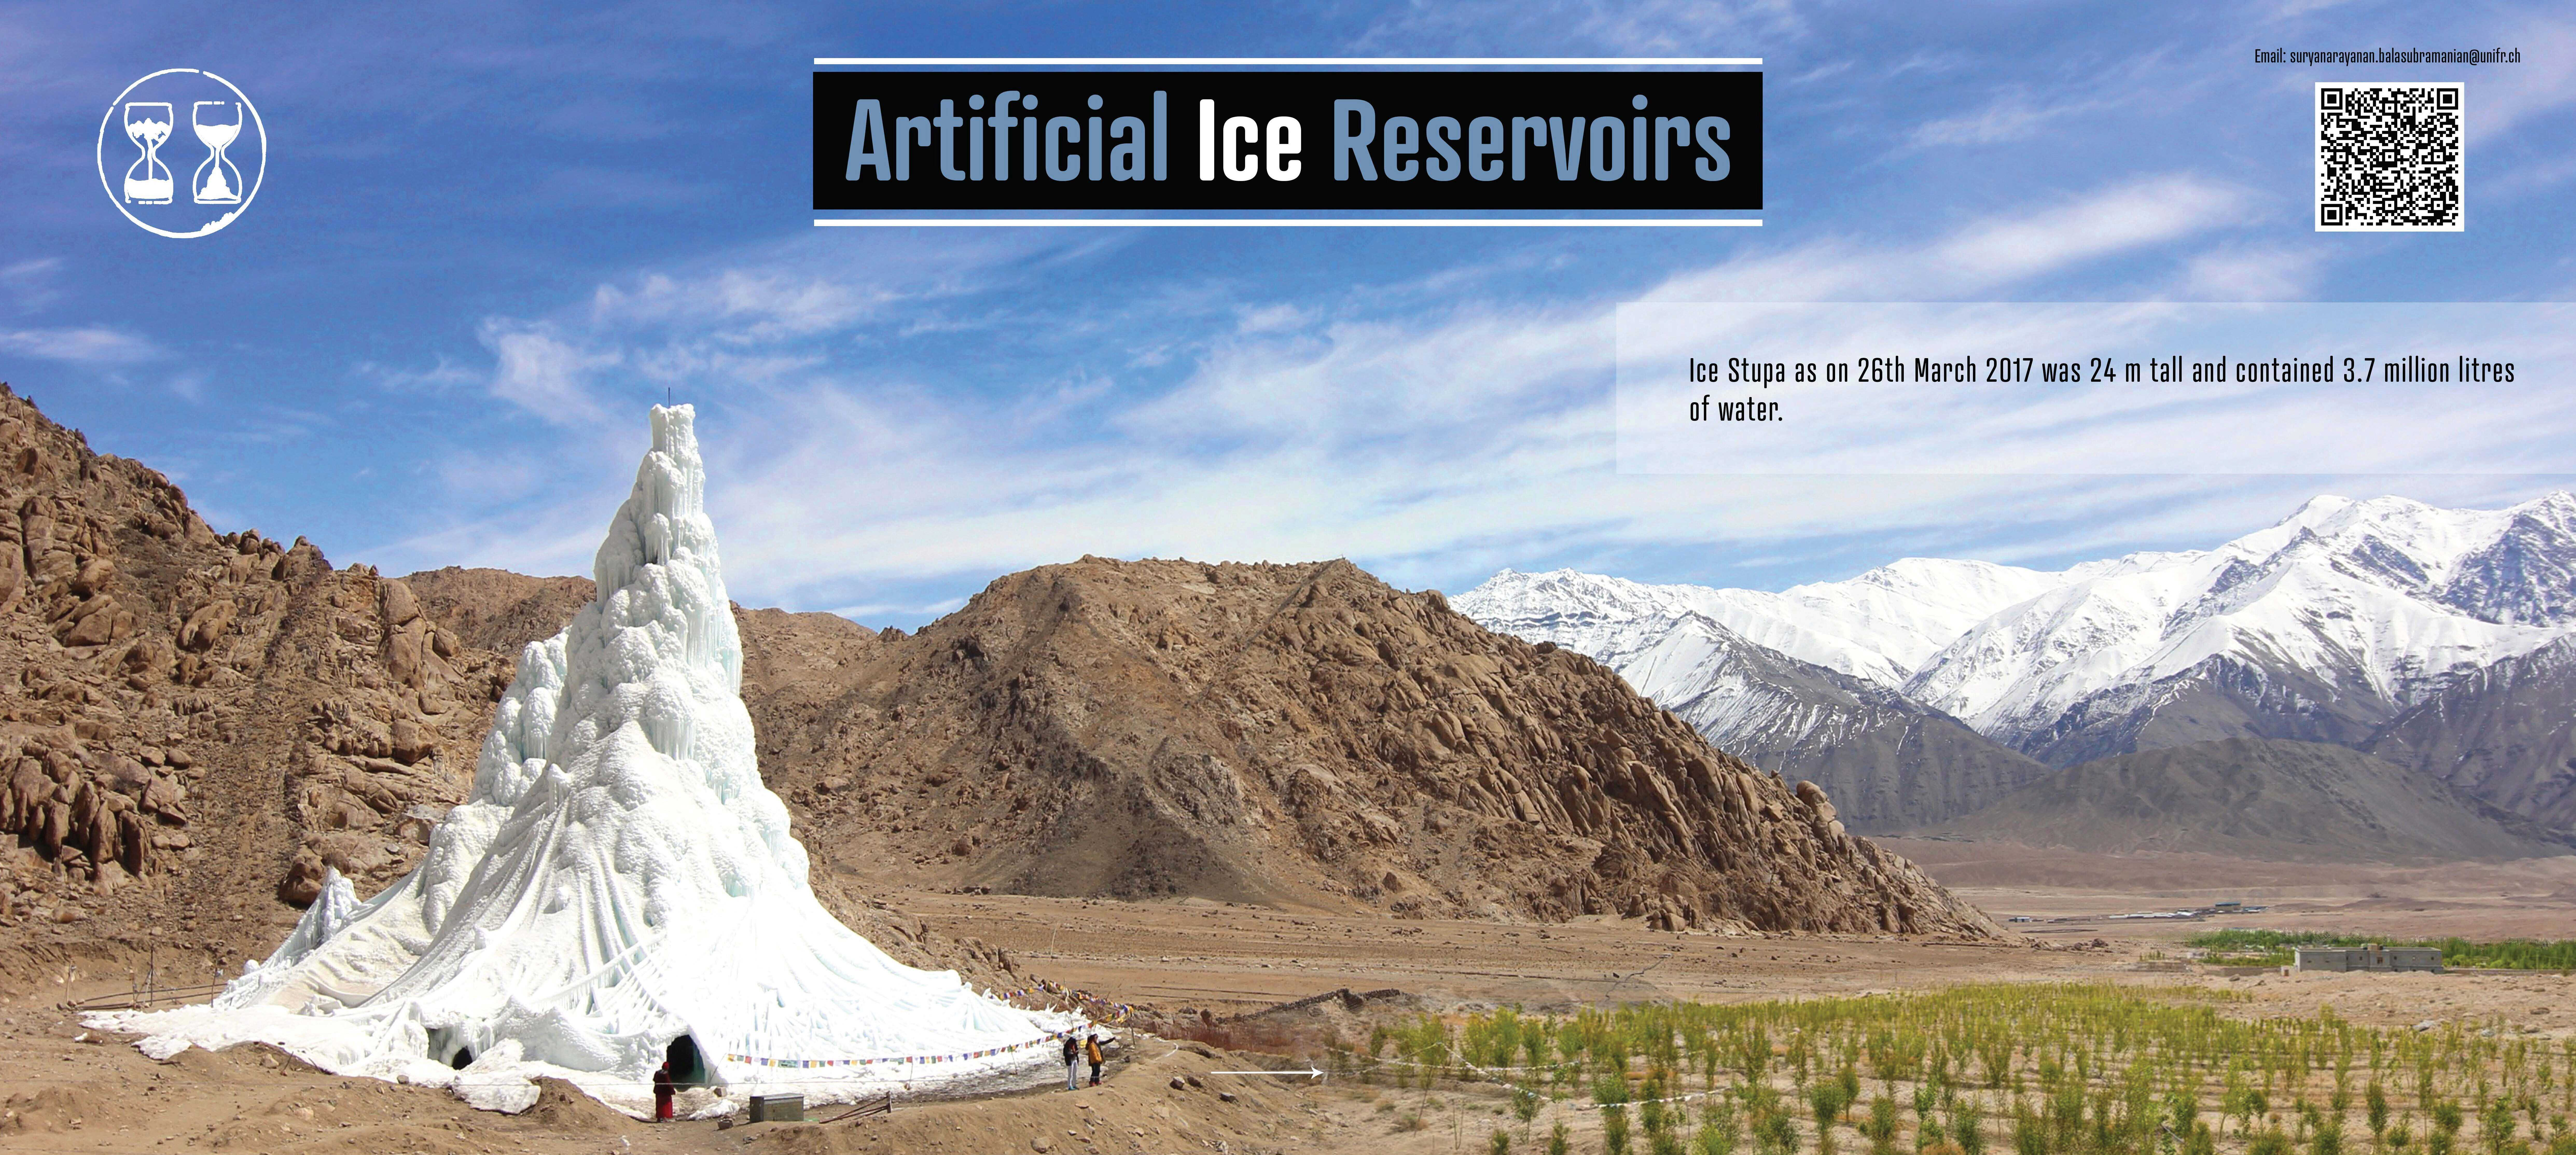
\includegraphics[width=\textwidth]{figs/AIR_title.jpg}
  \end{figure}
	{\Large\thesisTitle \par}
	\rule[5pt]{\textwidth}{.4pt} \par
	{\large\thesisName}
	\vfill
	\textit{\large\thesisDate} \\
	Version: \thesisVersion
\end{titlepage}


% ------------------------------------  --> main title page
\begin{titlepage}
	\pdfbookmark[0]{Titlepage}{Titlepage}
	\tgherosfont
	\centering

	% {\Large \thesisUniversity} \\[4mm]
	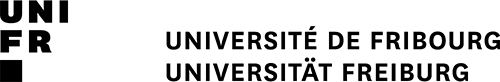
\includegraphics[width=6cm]{figs/unifr-logo} \\[2mm]
	\textsf{\thesisUniversityDepartment} \\
	% \textsf{\thesisUniversityInstitute} \\
	\textsf{\thesisUniversityGroup} \\

	\vfill
	\includegraphics[width=3cm]{figs/air_logo_circle} \\[2mm]
	% {\large \thesisSubject} \\[5mm]
	{\LARGE \color{ctcolortitle}\textbf{\thesisTitle} \\[10mm]}
	{\Large \thesisName} \\

	\vfill
	% \begin{minipage}[t]{.27\textwidth}
	% 	\raggedleft
	% 	\textit{1. Reviewer}
	% \end{minipage}
	% \hspace*{15pt}
	% \begin{minipage}[t]{.65\textwidth}
	% 	{\Large \thesisFirstReviewer} \\
	%   	% {\small \thesisFirstReviewerDepartment} \\[-1mm]
	% 	{\small \thesisFirstReviewerUniversity}
	% \end{minipage} \\[5mm]
	% \begin{minipage}[t]{.27\textwidth}
	% 	\raggedleft
	% 	\textit{2. Reviewer}
	% \end{minipage}
	% \hspace*{15pt}
	% \begin{minipage}[t]{.65\textwidth}
	% 	{\Large \thesisSecondReviewer} \\
	%   	% {\small \thesisSecondReviewerDepartment} \\[-1mm]
	% 	{\small \thesisSecondReviewerUniversity}
	% \end{minipage} \\[10mm]
	% \begin{minipage}[t]{.27\textwidth}
	% 	\raggedleft
	% 	\textit{3. Reviewer}
	% \end{minipage}
	% \hspace*{15pt}
	% \begin{minipage}[t]{.65\textwidth}
	% 	{\Large \thesisThirdReviewer} \\
	%   	% {\small \thesisThirdReviewerDepartment} \\[-1mm]
	% 	{\small \thesisThirdReviewerUniversity}
	% \end{minipage} \\[10mm]
	% \begin{minipage}[t]{.27\textwidth}
	% 	\raggedleft
	% 	\textit{4. Reviewer}
	% \end{minipage}
	% \hspace*{15pt}
	% \begin{minipage}[t]{.65\textwidth}
	% 	{\Large \thesisFourthReviewer} \\
	%   	% {\small \thesisFourthReviewerDepartment} \\[-1mm]
	% 	{\small \thesisFourthReviewerUniversity}
	% \end{minipage} \\[10mm]
	% \begin{minipage}[t]{.27\textwidth}
	% 	\raggedleft
	% 	\textit{Supervisor}
	% \end{minipage}
	% \hspace*{15pt}
	% \begin{minipage}[t]{.65\textwidth}
	% 	\thesisFirstSupervisor\
	% \end{minipage} \\[10mm]
	\begin{minipage}[t]{.27\textwidth}
		\raggedleft
		\textit{Supervisor}
	\end{minipage}
	\hspace*{15pt}
	\begin{minipage}[t]{.65\textwidth}
		{\Large \thesisFirstSupervisor} \\
	\end{minipage} \\[10mm]

	\thesisDate \\

\end{titlepage}


% ------------------------------------  --> lower title back for single page layout

This thesis was presented to the Faculty of Science of the University of Fribourg (Switzerland) in consideration
for the award of \textit{Doctor rerum naturalium} on \thesisDate.

\vfill
{\large \textbf{Citation} \\}
Balasubramanian, S. \thesisTitle . \thesisUniversityGroup, 2022.

\hfill
\vfill
{
	\small
	\textbf{\thesisName} \\
	\textit{\thesisTitle} \\
	\thesisSubject, \thesisDate \\
	Reviewers: \thesisFirstReviewer,\ \thesisSecondReviewer,\ \thesisThirdReviewer\ and \thesisFourthReviewer \\
	Supervisor: \thesisFirstSupervisor \\
	English editors: Lou Del Bello\ and Ana Rodríguez Crespo\\[1.5em]
	\textbf{\thesisUniversity} \\
	\textit{\thesisUniversityGroup} \\
	% \thesisUniversityInstitute \\
	\thesisUniversityDepartment \\
	\thesisUniversityStreetAddress \\
	\thesisUniversityCity \\
	\thesisUniversityPostalCode \\
  \url{https://www.unifr.ch/geo/cryosphere/en/}\\
\\
  This thesis was typeset with \LaTeXe.
  It uses the \textit{Clean Thesis} style developed by Ricardo Langner.
  Download the \textit{Clean Thesis} style at \url{http://cleanthesis.der-ric.de/}.
}

		% INCLUDE: all titlepages
\cleardoublepage
%
% % !TEX root = ../my-thesis.tex
%
\pagestyle{plain}
\pdfbookmark[0]{Preface}{Preface}
\addchap{Preface}

You can put your preface here.

\bigskip

\noindent\textit{\thesisUniversityCity, \thesisDate}

\smallskip

\begin{flushright}
	\begin{minipage}{5cm}
		\rule{\textwidth}{1pt}
		\centering\thesisFirstSupervisor
	\end{minipage}
\end{flushright}

%*****************************************
%*****************************************
 
% \cleardoublepage
%

\pagestyle{plain}				% display just page numbers
\pdfbookmark[0]{Summary}{Summary}
\addchap{Summary}
\label{sec:summary}

Irrigated agriculture is crucial for the livelihood security of mountain communities. Using meltwater from
glaciers, snow and permafrost, mountain dwellers have developed sophisticated techniques to cope with recurrent
water scarcity caused by glacial retreat, and seasonal snow-cover dynamics. Artificial ice
reservoirs (AIRs) are a key example of community based water management. Worldwide, farmers in around 30 mountain
villages build these ice structures. These seasonal ice reservoirs increase meltwater availability during the
critical period of water scarcity. To assess the role of AIRs within the water resource management of
mountain villages under a changing climate, they need to be represented in integrated modelling frameworks.
Efficient water storage can be achieved by taking into account their local meteorological conditions and
water availability throughout the year. This thesis aims to increase the understanding of volume dynamics of
AIRs in order to provide tools to reduce their water losses and maintenance requirements.

The different contributions of AIR surface processes built in Switzerland and Ladakh were estimated. These two
regions exhibit different meteorological patterns due to their significant latitudinal and altitudinal
differences. Using AIR-specific mass and energy balance models which keeps into account meteorological factors,
fountain discharge and ice volume changes, surface processes were quantified and compared across the two
locations. The models were successful in estimating the observed ice volume evolution with a root mean square
error within 20\% of the maximum ice volume for five AIRs. The location in Ladakh had a maximum ice volume four
times larger compared to the Guttannen site. However, poor fountain operation resulted in wastage of more than
four-fifth of the provided water supply. These results highlight the relevance of colder, drier climates and
fountain water supply management in optimizing AIR construction.

In addition, water loss reduction of AIRs on the Swiss Alps was attempted by implementing fountain scheduling
strategies. Fountain scheduling was realized through a control valve that was automated with optimal discharge
rates computed using customized glacial models. Simulations converting unscheduled fountains to scheduled
fountains showed a more than threefold improvement in the water use efficiency of several AIRs. Fountain
operation using scheduling strategies produced similar ice volumes while consuming one-tenth of the water
compared to their unscheduled counterparts.  Overall, these results show that automated fountain water supply
management can both increase the water use efficiency of AIRs and reduce their maintenance needs without
compromising on their meltwater production.

This thesis advances, for the first time, a model and measurement based understanding on the volume evolution of
AIRs under different climates. It provides tools to quantify the storage potential of these ice structures
worldwide and practical strategies to improve their efficacy. This study improves the scientific evidence needed
to upscale this indigenous water storage technology. These findings are essential to design these nature-based
solutions that increase the reliability of water supply in highly seasonal and arid environments and improve
water security and climate change adaptation in mountain regions. Future work may build on this research by
fully integrating climate change scenarios to investigate the potential hydrological contributions of ice
harvesting technologies for water-stressed mountain catchments.
		% INCLUDE: the abstracts (english and german)
\cleardoublepage

\currentpdfbookmark{\contentsname}{toc}
\setcounter{tocdepth}{1}		% define depth of toc
\tableofcontents				% display table of contents
\cleardoublepage

% --------------------------
% Body matter
% --------------------------
\pagenumbering{arabic}			% arabic page numbering
\setcounter{page}{1}			% set page counter
\pagestyle{scrheadings}			% header and footer style

%% Uncomment the following lines using the \part command
%% to add part sections
\chapter{Ice Reservoirs}

\cleanchapterquote{Glaciers are the secret of life in these otherwise lifeless deserts. But now, they are
	melting away at an alarming rate.}{Sonam Wangchuk}{(Ramon Magsaysay awardee,\\ Inventor of ice stupas)}


\section{Introduction}

Mountains contribute disproportionately to global water resources, considering their geographical extent.
Due to their buffering capacity, for instance by supplying glacial meltwater during the hot and dry season,
they provide a relatively constant water supply to downstream areas. Worldwide, the vast majority of glaciers
are losing mass \citep{zempGlobalGlacierMass2019a}, snow melt dynamics are being perturbed
\citep{mukhopadhyayReevaluationSnowmeltGlacial2015, hammondGlobalSnowZone2018}, and precipitation and
evapotranspiration patterns are shifting; all these leading to future vulnerability of mountain water availability
\citep{lutzConsistentIncreaseHigh2014}. These changes are believed to be largely and negatively
impacting agriculture across many different mountainous regions \citep{ipccCrossChapterPaperMountains2022}.

These issues are particularly pronounced in arid and semiarid regions, where it is estimated that between 50 \%
and 90 \% of freshwater resources originate from mountain catchments
\citep{mukhopadhyayReevaluationSnowmeltGlacial2015, messerliMountainsWorldVulnerable2004}. As a consequence,
mountain communities have developed some nature-based water storage solutions and farming practices, namely,
bofedales \citep{monge-salazarEcohydrologyEcosystemServices2022}, amunas
\citep{ochoa-tocachiPotentialContributionsPreInca2019}, rock glacier oasis \citep{pandeyRockGlacierOasis2022},
and \ac{AIRs} \citep{wangchukIceStupaCompetition2020} to cope with climate-change-induced water stress.

\citet{immerzeelImportanceVulnerabilityWorld2020} quantify the importance of these mountain regions by
classifying river basins as \ac{WTUs}. Globally, a total of 78 \ac{WTUs} are home to more than 250 million
people. Among these, the most important WTUs lie in \ac{HMA}, where communities are increasingly relying on
\ac{AIRs} for climate change adaptation (Fig. \ref{fig:WTUs_AIRs}). 

\ac{AIR} building is a long tradition, with records dating back more than 50 years
\citep{nusserSociohydrologyArtificialGlaciers2019}. \ac{AIRs} capture water in the autumn and winter, allowing
it to freeze and holding it until spring, when it melts and flows down to the fields
\citep{ipccChapterHighMountain2019, vinceGlacierMan2009, clouseLadakhArtificialGlaciers2017,
nusserSociohydrologyArtificialGlaciers2019}. In this way, they retain an otherwise unused portion of annual
flow and facilitate its use, supplementing the decreased flow during the following spring (Fig.
\ref{fig:irrigation_cycles}). Over the past decade, several \ac{AIRs} have been built to supplement the
irrigation water supply of mountain villages in India \citep{wangchukIceStupaCompetition2020,
palmerStoringFrozenWater2022, aggarwalAdaptationClimateChange2021}, Pakistan
\citep{awazproductionIceStupaArtificial2022}, Kyrgyzstan \citep{bbcnewsBrightArtificialGlacier2020}, Nepal, and
Chile \citep{reutersConservationistsChileAim2021}. In total, more than 500 farmers have constructed AIRs across
30 villages in the Alps, Andes, and Hindu Kush Himalayas (Fig. \ref{fig:WTUs_AIRs}).

\begin{figure}[htb]
	\centering
	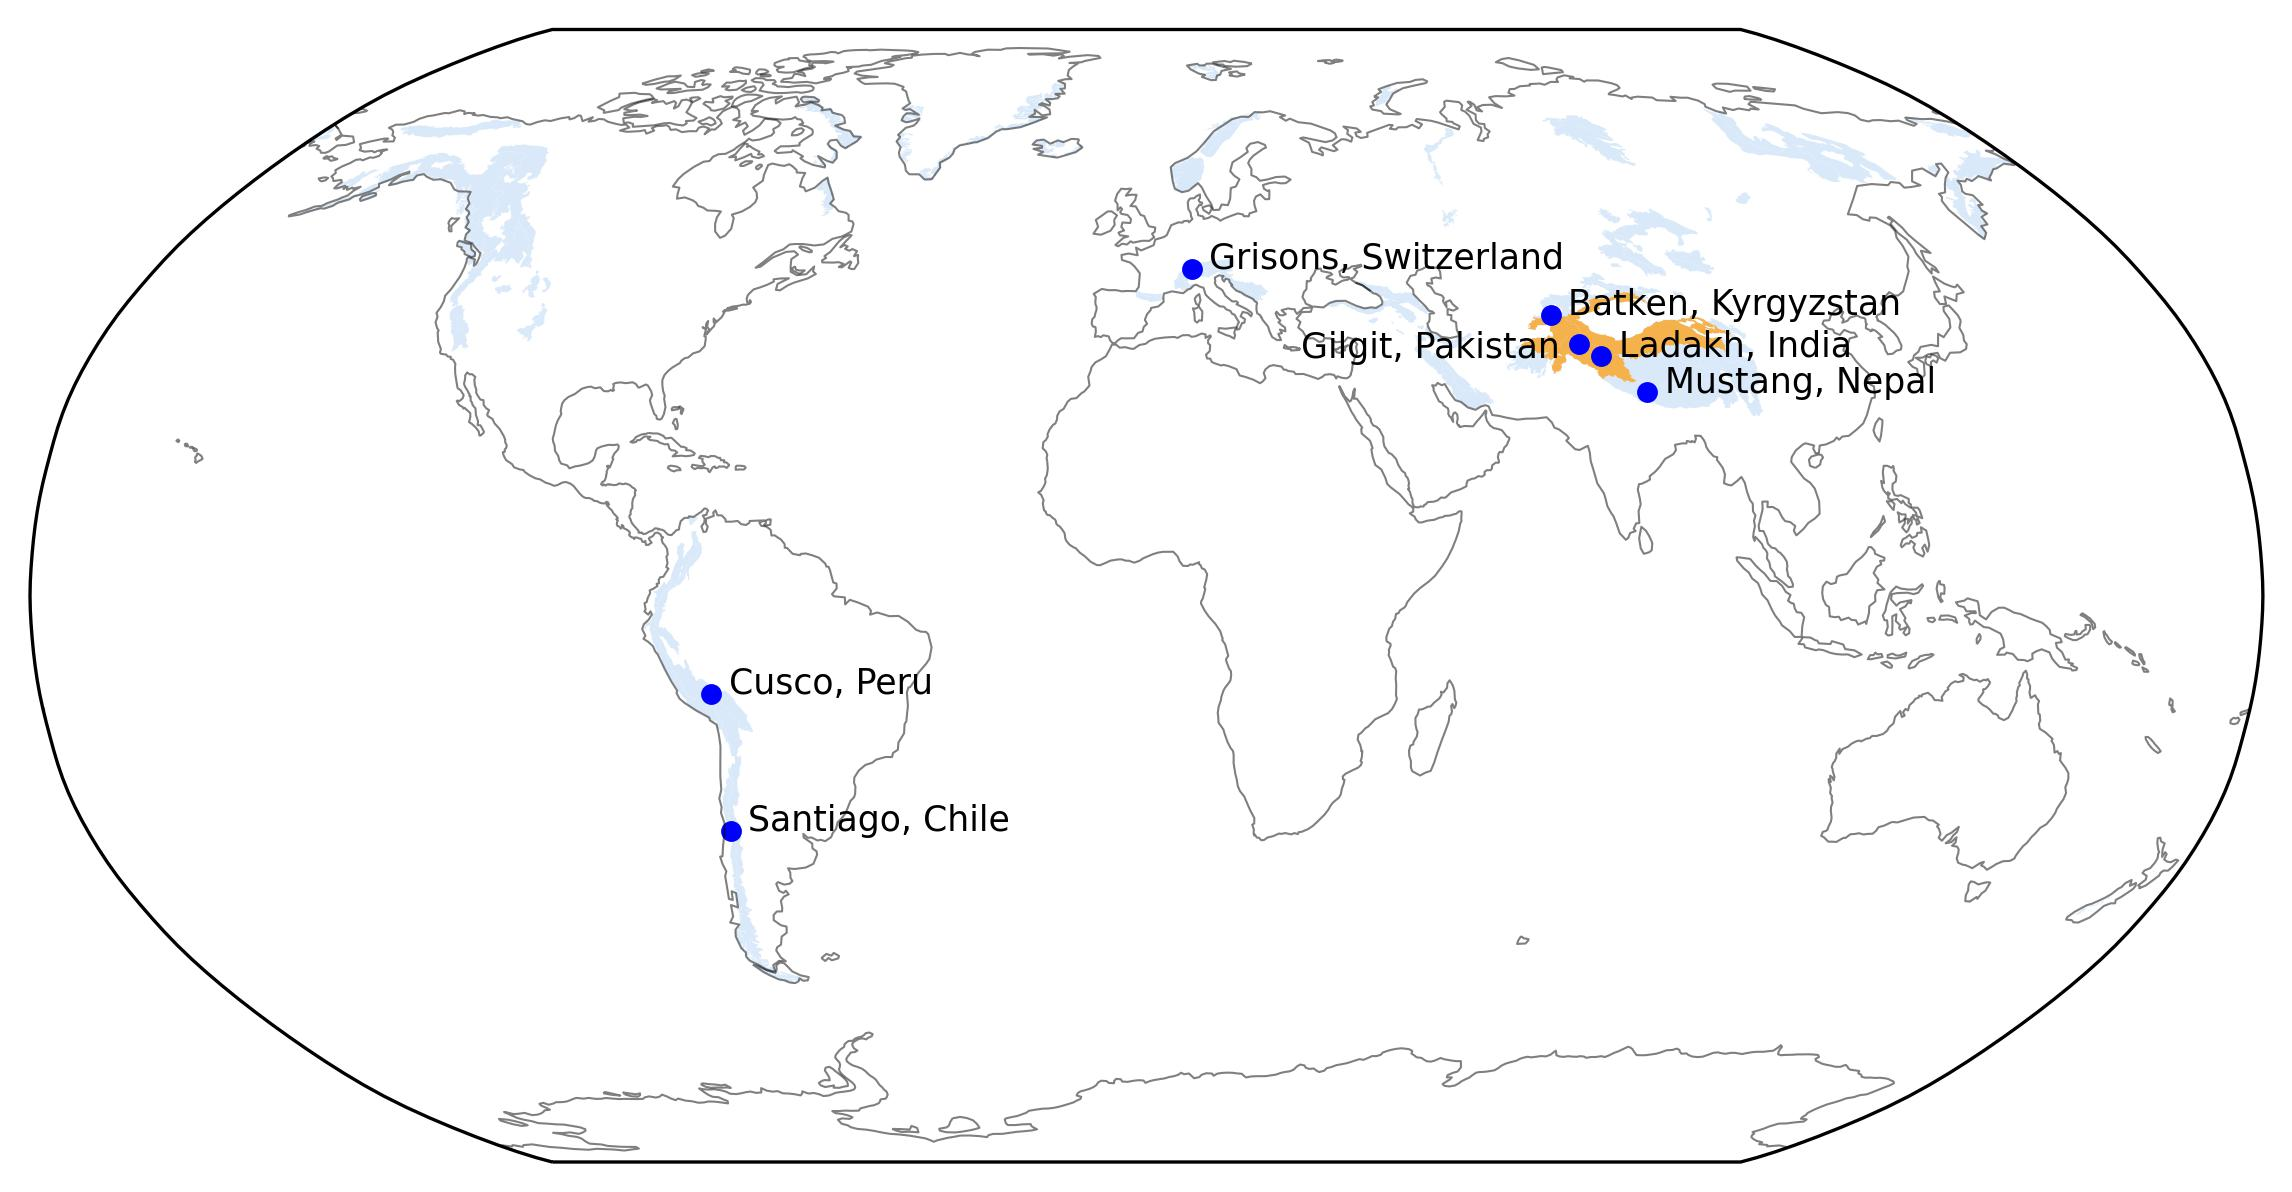
\includegraphics[width=\textwidth]{figs/WTUs_AIRs.jpg}

	\caption{ Global distribution of water tower units (light blue) based on
		\citet{immerzeelImportanceVulnerabilityWorld2020}. The most important \ac{WTUs} (orange) are also situated where most 
		AIR construction sites  are located (dark blue). }

	\label{fig:WTUs_AIRs}
\end{figure}

\begin{figure}[htb] \centering 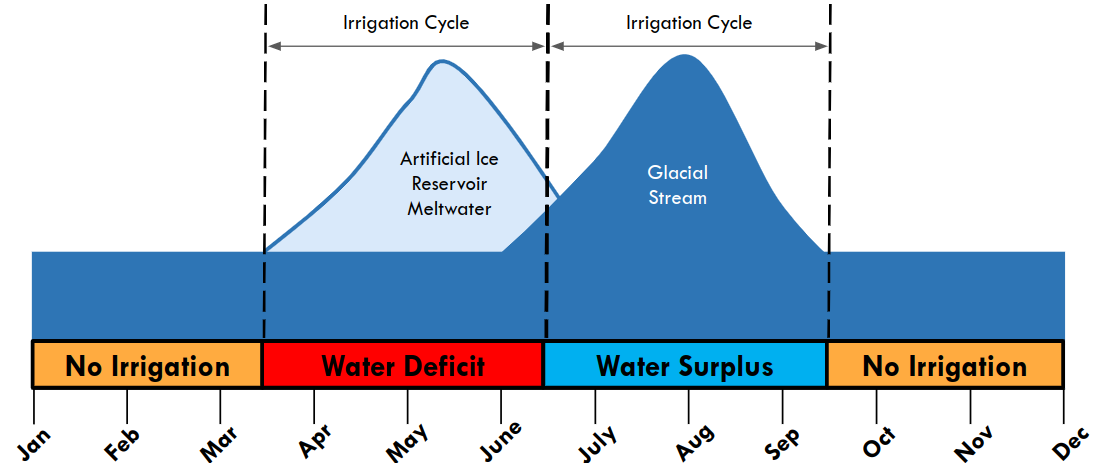
\includegraphics[width=\textwidth]{figs/irrigation_cycles.png}
	\caption{Seasonal variation in availability of irrigation water in Ladakh, India. The graph highlights the
		crucial role of \ac{AIRs} in bridging the gap in water availability. Adapted from
		\citet{nusserLocalKnowledgeGlobal2016}.} \label{fig:irrigation_cycles} \end{figure}


Despite this widespread adoption, only a few publications have examined the role of \ac{AIRs} in the water resource
management of these regions. Notably, none of these prior reports have investigated \ac{AIRs} outside Ladakh.
Moreover, the available estimates of water storage capacity of \ac{AIRs} in Ladakh vary widely
\citep{norphelSnowWaterHarvesting2015, baglaArtificialGlaciersHelp1998}.

Quantifying the water storage capacity of \ac{AIRs} is not straightforward, since the processes by which
\ac{AIRs} are formed are complex. These processes are controlled by local topography, meteorology, and the
construction strategies used. Modelling approaches to quantify these processes exist on glacier surfaces, but
they are not readily applicable for \ac{AIRs} due to their limited size and their comparatively more variable surface
area. Therefore, conventional modelling approaches used in glaciology need to be adapted to capture the
spatiotemporal scale of AIR surface processes. Furthermore, these modelling approaches need to be validated and
calibrated with comprehensive data from field measurements.

A spirit of improvisation guides the construction of \ac{AIRs} \citep{clouseLadakhArtificialGlaciers2017}.
Depending on the local topography and on how water is supplied, \ac{AIRs} can form as flat sheets or vertical
cones, and are therefore referred to as ice terraces or ice stupas, respectively (Fig. \ref{fig:AIRforms}). This
resuls in \ac{AIRs} exhibiting significant volume variations despite experiencing similar
meteorological conditions. For example, in Ladakh, India, ice terraces have attained volumes up to 30 times
larger than ice stupas \citep{nusserSociohydrologyArtificialGlaciers2019}. However, the processes driving these
differences can only be understood if the complete design methodology behind each construction is available.

\begin{figure}[t]
	\centering
	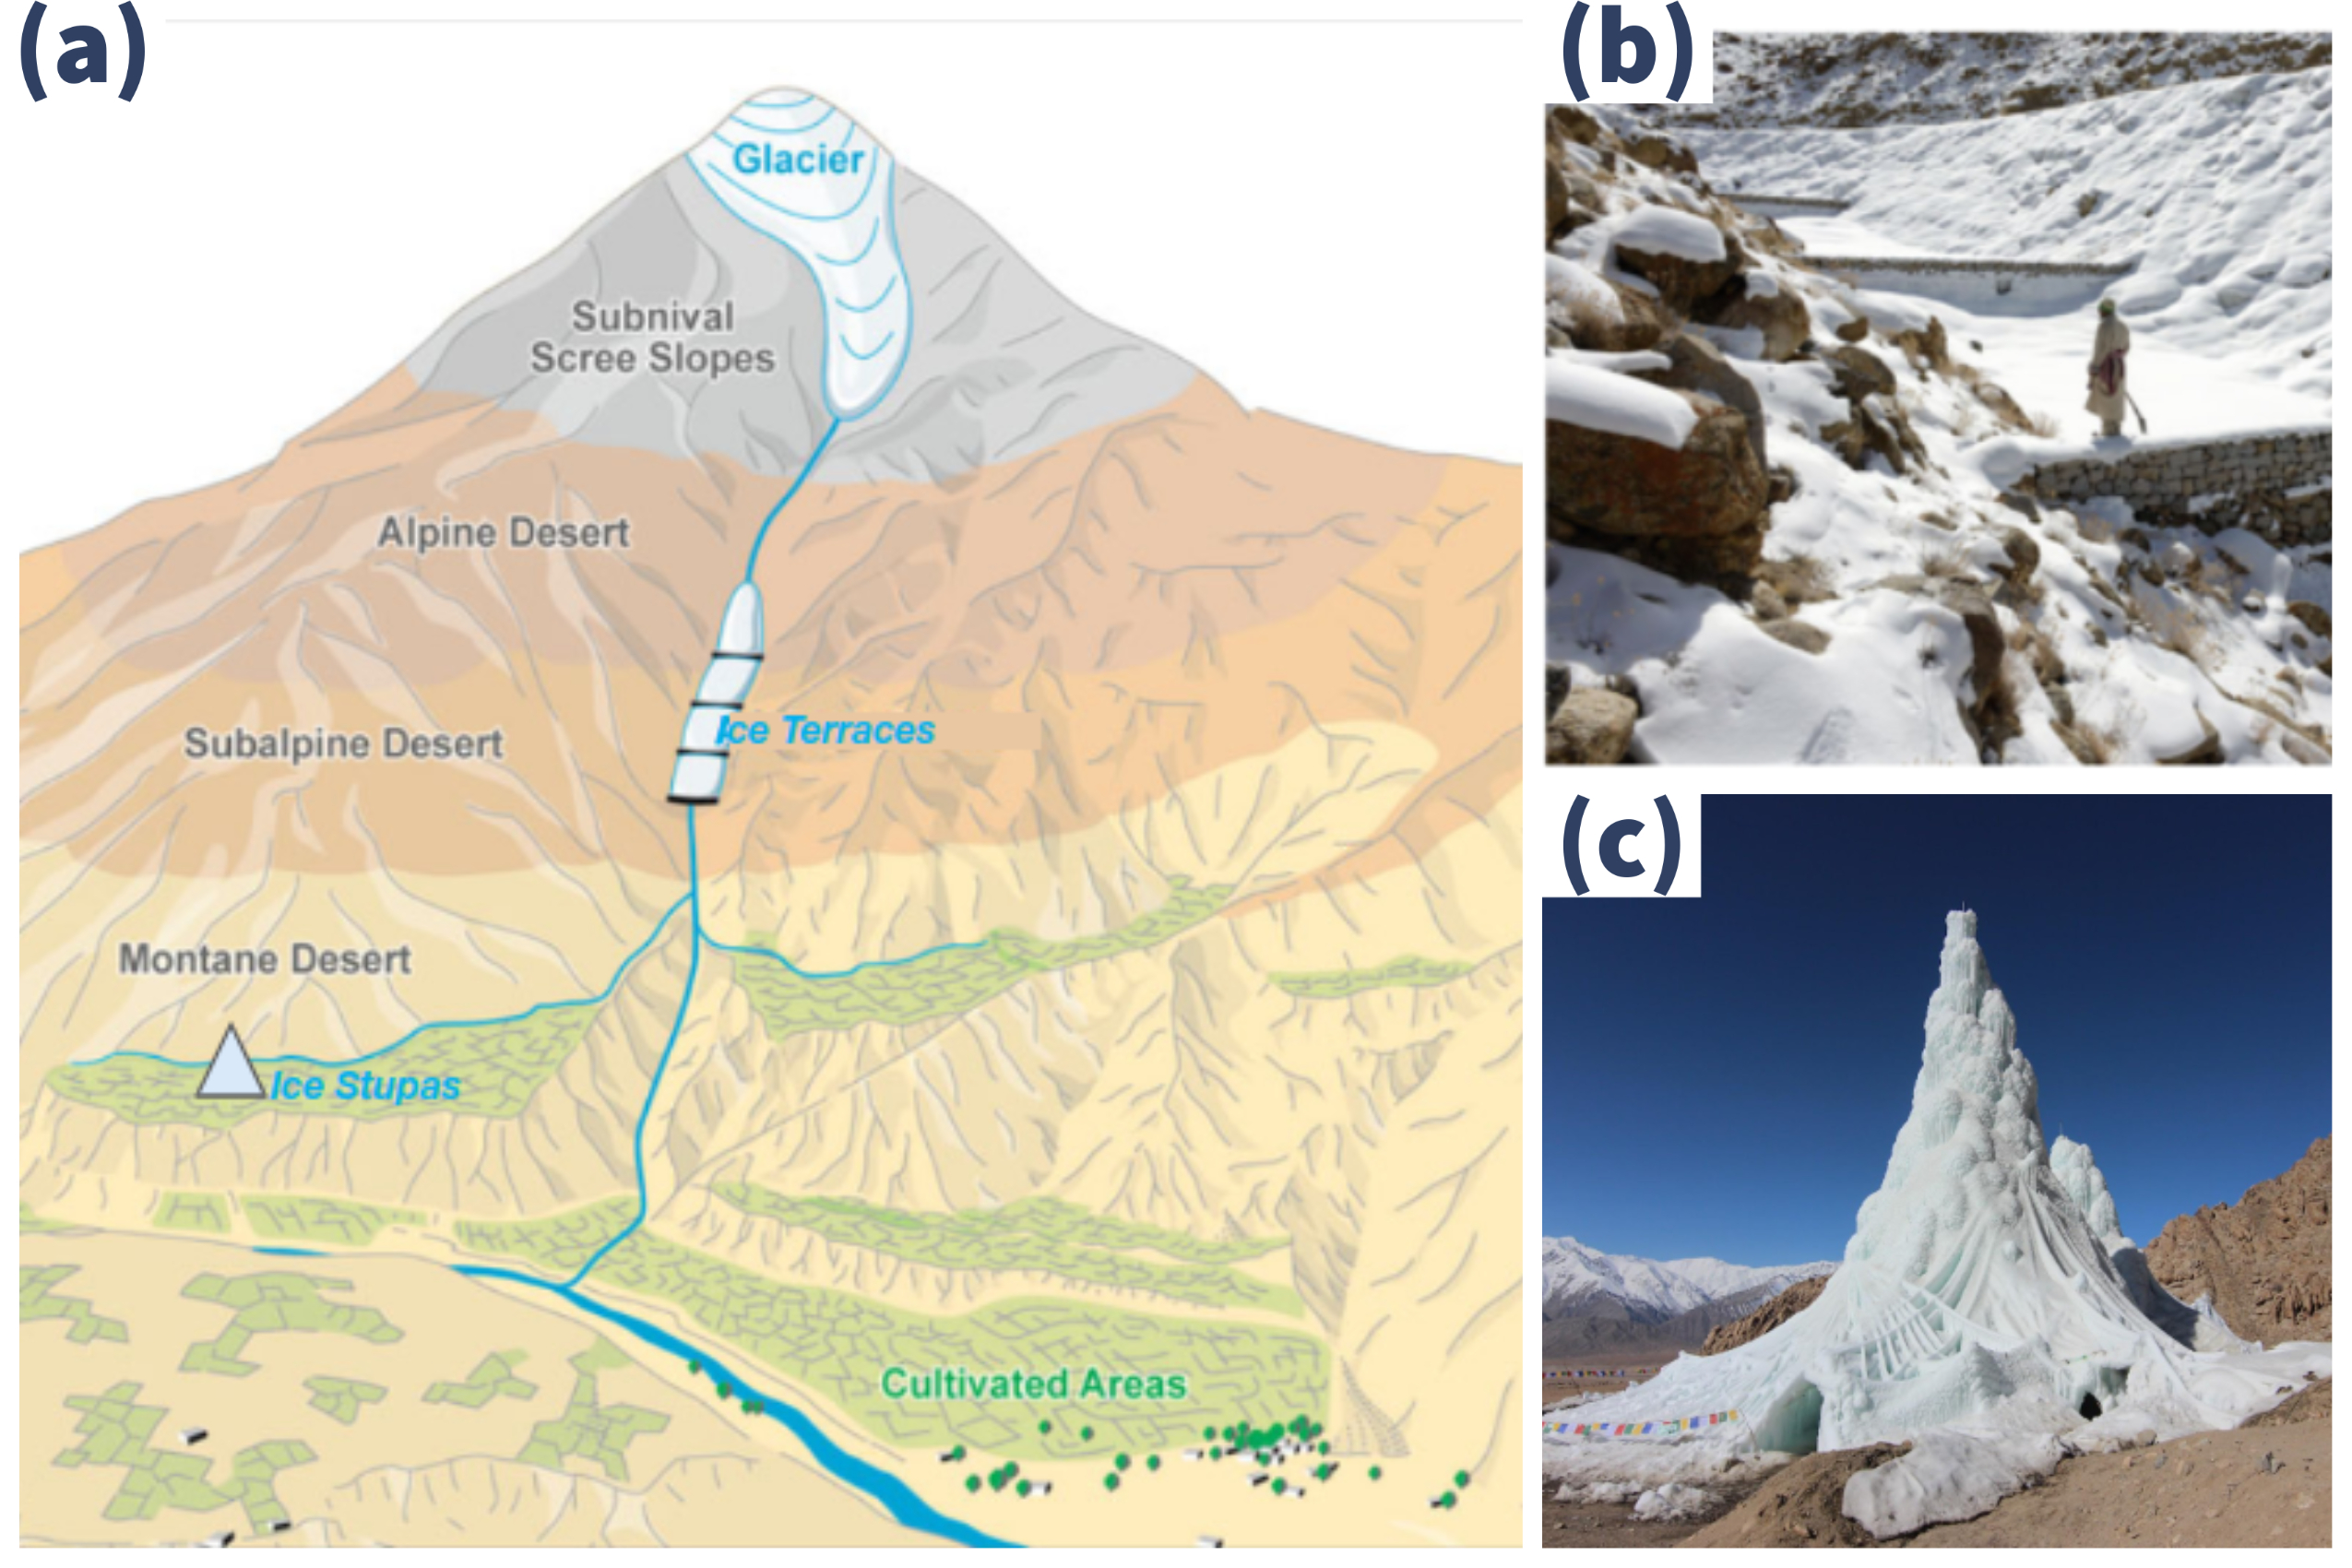
\includegraphics[width=\textwidth]{figs/AIR_forms.jpg}

	\caption{ (a) Schematic overview of the position of artificial ice reservoirs. These constructions are located at
		altitudes between the glaciers and the irrigation networks in the cultivated areas. (b) Ice terraces at 3900
		$m$ \ac{a.s.l.}, located above the village of Nang, Ladakh. The cascade is composed of a series of loose masonry walls
		ranging in height from 2 to 3 $m$, which facilitate the freeze of water for storage. (c) Ice stupas at 3600 m, located
		above the village of Phyang, Ladakh. They are constructed using fountain systems. Adapted from \citet{nusserLocalKnowledgeGlobal2016}. }

	\label{fig:AIRforms}
\end{figure}

This thesis aims to fulfill the abovementioned requirements by providing a new set of AIR-specific volume and area
measurements via drone flights, along with meteorological data recorded during the construction period. All these
datasets are obtained from construction strategies that involve fountain systems. These systems are quantified
via \textit{in situ} observations of the fountain characteristics and discharge rate measurements. First, one- and two-dimensional models are formulated, calibrated, and validated with the procured AIR datasets. Then,
these models are used as tools to propose a construction strategy that can produce \ac{AIRs} efficiently and
effortlessly. While this thesis reviews published research, substantial additional knowledge is held by the
farming communities building these structures since the mid-1800s.


\section{Nomenclature and classification}

The term "artificial glacier" is commonly used by local farmers to refer to \ac{AIRs}
\citep{norphelArtificialGlacierHigh2009}. However, many believe this term can be misleading
\citep{nusserSociohydrologyArtificialGlaciers2019}. By definition, all glaciers, including the smallest ones,
are bodies of sedimentary ice built by progressive snow compaction and firnification that flow
downhill under the influence of gravity \citep{benndouglasGlaciersGlaciation2014}. Hence, because of their
genesis and composition, \ac{AIRs} differ from glaciers. Human-made ice structures typically have a lifetime in
the order of months and a size a million times smaller than natural glaciers. The term \ac{AIRs} is used in this thesis to
distinguish the man-made ice structures described above from the natural ones.

However, when classified in terms of size and survival duration, \ac{AIRs} exhibit similar characteristics to
very small glaciers. The glossary of glacier mass balance and related terms by
\citet{cogleyGlossaryGlacierMass2010} defines very small glaciers or glacierets as follows:

\begin{thesis_quotation}
	A very small glacier, typically less than 0.25 $km^2$ in extent, with no marked flow pattern
	visible at the surface. To qualify as a glacieret, an ice body must persist for at least two consecutive
	years. Glacierets can be of any shape, and usually occupy sheltered parts of the landscape. Windborne snow and
	avalanches can be dominant contributors to the accumulation of glacierets.
\end{thesis_quotation}

This rather broad definition of glacierets or very small glaciers may be best suited to describe AIRs, since
they present areas as large as 0.15 $km^2$ \citep{nusserSociohydrologyArtificialGlaciers2019} and
have been observed to last beyond a year.

As noted above, AIR's construction strategies are usually inspired by a spirit of improvisation, which challenges
their classification. However, construction strategies using fountain systems have been found to form
conical \ac{AIRs}, while others form flat sheets of ice. \ac{AIRs} using fountain systems are called
"ice stupas", and those not using them are called "ice terraces"; this terminology denotes the resulting shape of the
respective \ac{AIRs}.

\section{Research aim and outline}

The preceding sections show that many of the small-scale surface processes that occur on \ac{AIRs} are complex
and not well understood at present and that their interplay remains uncertain. These need to be unraveled to be able to better predict the
water storage potential of \ac{AIRs} and to improve their water storage efficiency under different climate conditions and with different
construction methodologies. Therefore, the main objective of the present thesis is:

\begin{thesis_quotation}

  \textbf{To increase the understanding of volume dynamics of artificial ice reservoirs to
  provide tools that reduce their water losses and maintenance requirements.}

\end{thesis_quotation}

Data on \ac{AIRs} are scarce, which is the reason for many of the unknowns and uncertainties around the dynamics
of these ice structures. This thesis therefore has a strong focus on the implementation of measurement campaigns
using drones and \ac{AWS} to achieve its main objective. The thesis touches on two different topics that
address the following specific research questions:

\begin{enumerate}

  \item \textit{What is the influence of construction location and fountain characteristics on ice stupa volume
    evolution?}

Three process-based models for ice stupas were designed to answer the first research question. Since \textit{in situ}
    measurements were required to run this model, measurement campaigns were executed in Switzerland and India
    during the past four winters (2018/19, 2019/20, 2020/21, and 2021/22). These datasets provided the necessary
    input, calibration, and validation data to model the evolution of ice stupas and study their sensitivity to
    meteorological conditions and fountain characteristics. Description of the study sites and overview of these
    models are presented in the \textit{Science} chapter. Results from their application are presented in the
    \textit{Habitat} chapter.

  \item \textit{How can ice stupa fountain systems be engineered to reduce water losses and maintenance
    efforts?}

To answer this question, a new construction strategy was developed using an automation system. The automation
    hardware incorporated the models developed to regulate fountain discharge rate. The description of the
    automation system and its advantages over manual construction strategies are presented in the
    \textit{Technology} chapter.

\end{enumerate}

In addition to the chapters mentioned above, the \textit{Religion} chapter illustrates the origin of ice harvesting
solutions among mythologies and religious practices; in the \textit{Heritage} chapter, the main findings
presented in this thesis are placed into a broader perspective through some recommendations; and the
\textit{Papers} chapter lays out the peer-reviewed work supporting this thesis.


   % INCLUDE: introduction
\chapter{Religion of ice reservoirs}

\cleanchapterquote{We believe that glaciers are alive. That's why a combination of
female and male ice was necessary.}{Liaquat Ali Baltee}{(Resident of Skardu, Pakistan)}

For centuries, in the Himalayan mountain ranges, local cultures have believed that glaciers are alive and that
certain glaciers can also have different genders. These local communities ‘breed’ new glaciers by grafting
together —or marrying— fragments of ice from male and female glaciers covering them with charcoal, wheat husks,
cloths, or willow branches so they can reproduce in privacy. These glacierets transform into fully active
glaciers by growing year by year with additional snowfall, serving as lasting reservoirs of water that allow
farmers to irrigate their crops. Over time, these practices have inspired other cultures, in which people are
now creating their own \ac{AIRs} and using them to solve urgent challenges around water supplies.

\section{An old story}

According to legend, when the people of Baltistan, in Pakistan, learnt of the Mongol army advancing towards them
from the north in the early $13^{th}$ century, they came up with an ingenious way to stop them. As the inhabited
valleys were only accessible through narrow passes, they decided to block the entry way by building a glacier.
This successfully prevented the Mongol invasion and, crucially, also solved the locals’ other big problem: water
scarcity \citep{khanMarriageGlaciersPrzekroj2020}.

\section{The marriage of glaciers}

The people of Gilgit Baltistan believe that glaciers are living entities
\citep{farazGlacierMarriagesPakistan2020, khanMarriageGlaciersPrzekroj2020}. Therefore, a combination of female
and male ice is absolutely necessary for them to multiply and grow. The male glacier –locally called ‘po gang’–
gives off little water and moves slowly, while a ‘female glacier’ –or ‘mo gang’– is a growing glacier that gives
off a lot of water. 

The glaciers that people help grow are the fruit of the sacred union between a mother glacier and a father
glacier. The ice formations get married and produce offspring. For local communities, the selection of an
appropriate site for this marriage is of utmost importance, and a suitable site must fulfil a list of
conditions. It should be located at an altitude of at least 4000 to 5000 m \ac{a.s.l.} and should be on a gentle
slope with minimal exposure to sunlight, thus a north-facing mountain side is preferable. For most expert
glacier grafters, the presence of permafrost or ice on the site is another key requirement. 

Once a suitable spot is selected, the expedition can be planned. The bride and groom---the female and the male
glacier, preferably from different villages---are chosen, and the marriage can be organized. The glacier
grafting usually takes place in November, when the local temperatures oscillate around zero. The process used to
conduct this glacier marriage ceremony is described in \citet{khanMarriageGlaciersPrzekroj2020} as follows:

A 12-man party carries the pieces of female ice in woven baskets. Another 12 men carry the male ice. The water
drawn from the Indus river is carried traditionally in 12 gourd bottles, but sometimes clay pots or goatskins
are also required, so are charcoal and wheat husks or sawdust, which act as insulators for the ice. The last
ingredient is salt, which, according to some glacier grafters, helps protect the new glacier from impurities.
The bride and groom party walk from different sites and meet at a certain point to climb together to their
destination, where the new glacier will be created. No greetings are exchanged, as the people involved in the
ceremony must remain silent until the ice is deposited in its new home. They walk continuously without
any breaks, but if the distance is too much and rest is required, they do not put their loads on the ground;
instead, they hang the baskets on trees, or on walking sticks if nothing else is available. Each man must
carry around 15 to 25 $kg$ of ice, walking in the cold air, silently up the mountains, for a day or more. Once
they reach the glacier growing site, they deposit their valuable loads. The ice lumps and water vessels are
placed in between the boulders---or in a small cave or sometimes in a pit dug specifically for this purpose---and
are covered with layers of salt, charcoal, and sawdust. The silence is finally broken as religious leaders recite
verses of the Quran and pray for the success of the glacier marriage and for protection from the \textit{djinns}. Once
the male and female glaciers are placed in their new home and covered, a man from the glacier grafters' party
stands up and offers his life for the success of the process. His symbolic sacrifice is matched by the actual
sacrifice of a goat---its meat distributed to a charity because prayers are more likely to be answered if
accompanied by a charitable act. They will not visit the place for at least 3 years, so as not to disturb
the glacier. It is said that a person who disturbs the glacier before its maturation will die. The celebrations
continue in the village with traditional songs and prayers, alongside festive food and the joy of the
accomplished mission.

\section{From folklore to science}

Myths, legends, and superstitions are ways of codifying and disseminating knowledge. However, in the face of a
mounting climate crisis, they now need to be translated into the language of science. 

Classifying glaciers as male and female is, of course, a practice motivated by deep religious beliefs, but the
method used to achieve this classification hints at an even deeper understanding of their temporal discharge
patterns. In scientific terms, male glaciers are those which have achieved their peak water, likely leading to
imminent water scarcity in their catchment. The concept of 'peak water' implies that, first, as glaciers shrink
in response to a warmer climate, more meltwater is released until a turning point (peak water), after which
glaciers melt, and so its contribution to river flow decreases. Based on this perspective, accelerated glacier
shrinkage due to climate change is causing a gender imbalance. Such narratives are not designed to stand up to
scientific scrutiny but rather to illustrate the state of the world in the most simple and effective way that
can inspire societal change. 

However, when it comes to glacier building expeditions, the evidence available is scant and anecdotal. According
to \citet{tveitenGlacierGrowingLocal2007}, the account of the glacier development process presented by a glacier
grafter from the Baltistan region bears a strong resemblance to the definition of the formation of rock
glaciers. \citet{tveitenGlacierGrowingLocal2007} concludes that: 

\begin{thesis_quotation}

“glacier growing is typically performed […] in a terrain that is conducive to the accumulation of snow by
avalanching and snow slips. The presence of permafrost at these locations is likely to contribute to ice
accumulating […]. Thus, glacier growing is conducted at locations which are already very prone to ice
accumulation, and may explain why glacier growing is perceived to work.” 

\end{thesis_quotation}

Therefore, the practices involved in glacier grafting do not have scientific evidence to support their efficacy
in building artificial glaciers. Still, they have been an effective tool to communicate the effects of glacier
shrinkage and instigate action for their preservation across regional and global scales. 

The view of glaciers as animate entities implies that humans can influence their lives, just as glaciers can
influence the lives of people. A fact that much of the world is still catching up to.

These mythologies and practices from Baltistan, Pakistan inspired local engineers in Ladakh, India to try
conserving winter water supply as ice structures. Despite the two regions being in different countries, the
geographic and cultural proximity of the communities paved the way for the further development of these
practices in Ladakh.
   % INCLUDE: related work
\chapter{Science of ice reservoirs}
\label{chap:science}

\cleanchapterquote{I could do with some scientific help from specialists. I am trying to collect data on how and
  where glaciers form best so that I can improve on them and people can use the technique elsewhere.
}{Chewang Norphel}{(Padmashree awardee, Inventor of ice terraces)}

This chapter provides the methodology used to estimate the ice volume evolution and water-use efficiency of
AIRs. The equations governing the mass and energy balance of ice stupas is explained along with the associated
datasets required for forcing, calibration and validation of this AIR model.

% In a first step, the influence of the chosen location and fountain used was quantified by feeding weather and
% fountain data to an energy balance model and validating the ice volume estimates produced with volume
% observations from drone flights. In a second step, the model was extended to serve as a tool for recommending
% discharge rates and identifying favourable construction locations worldwide.

\section{Study sites and data}

\subsection{Study sites}

We chose two villages in the Swiss Alps and the Indian Himalayas called Guttannen and Gangles to collect the
required datasets described above. The study period starts when the fountain was first switched on and ends when
the respective AIR either melted or broke into several ice blocks. These two dates are denoted as start and
expiry dates henceforth. Each AIR dataset was abbreviated based on the construction strategy used, prefix of the
country code and the suffix of the year of its expiry date. The construction strategies are distinguished based
on whether they used fountain scheduling strategies to regulate water supply. Those that did were codenamed
automated construction strategy whereas the rest were codenamed traditional construction strategy. In total,
five AIRs were studied in these two locations across three winters (see Table \ref{tab:AIRs}). Only one was
built in Gangles. The rest were built in Guttannen. All except one construction campaign used traditional
construction strategies. Therefore, traditional AIRs are referred to without explicitly specifying their
construction strategy henceforth.

The Guttannen site (46.66 $\degree$N, 8.29 $\degree$E) is situated in the Berne region, Switzerland and has an
altitude of 1047 $m$ a.s.l. In the winter (Oct-Apr), mean daily minimum and maximum air temperatures vary
between -13 and 15 $\degree C$. Clear skies are rare, averaging around 7 days during winter. Daily winter
precipitation can sometimes be as high as 100 $mm$. These values are based on 30 years of hourly historical
weather data measurements \citep{meteoblueClimateGuttannen2021}. Several AIRs were constructed by the Guttannen
Bewegt Association, the University of Fribourg and the Lucerne University of Applied Sciences and Arts during
the winters of 2020-22.

The Gangles site (34.22 $\degree$N, 77.61 $\degree$E) is located around 20 km north of Leh city in the Ladakh
region, lying at 4025 $m$ a.s.l.. The mean annual temperature is $5.6 \, \degree C$, and the thermal range is
characterized by high seasonal variation. During January, the coldest month, the mean temperature drops to $-7.2
\, \degree C$. During August, the warmest month, the mean temperature rises to $17.5 \, \degree C$
\citep{nusserIrrigationDevelopmentUpper2012}. Because of the rain shadow effect of the Himalayan Range, the mean
annual precipitation in Leh totals less than 100 $mm$, and there is high interannual variability. Whereas the
average summer rainfall between July and September reaches 37.5 $mm$, the average winter precipitation between
January and March amounts to 27.3 $ mm$ and falls almost entirely as snow. AIRs were constructed here as part of
the Ice Stupa Competition by the Himalayan Institute of Alternatives, Ladakh (HIAL). 

% \begin{figure}
%   \centering
% 	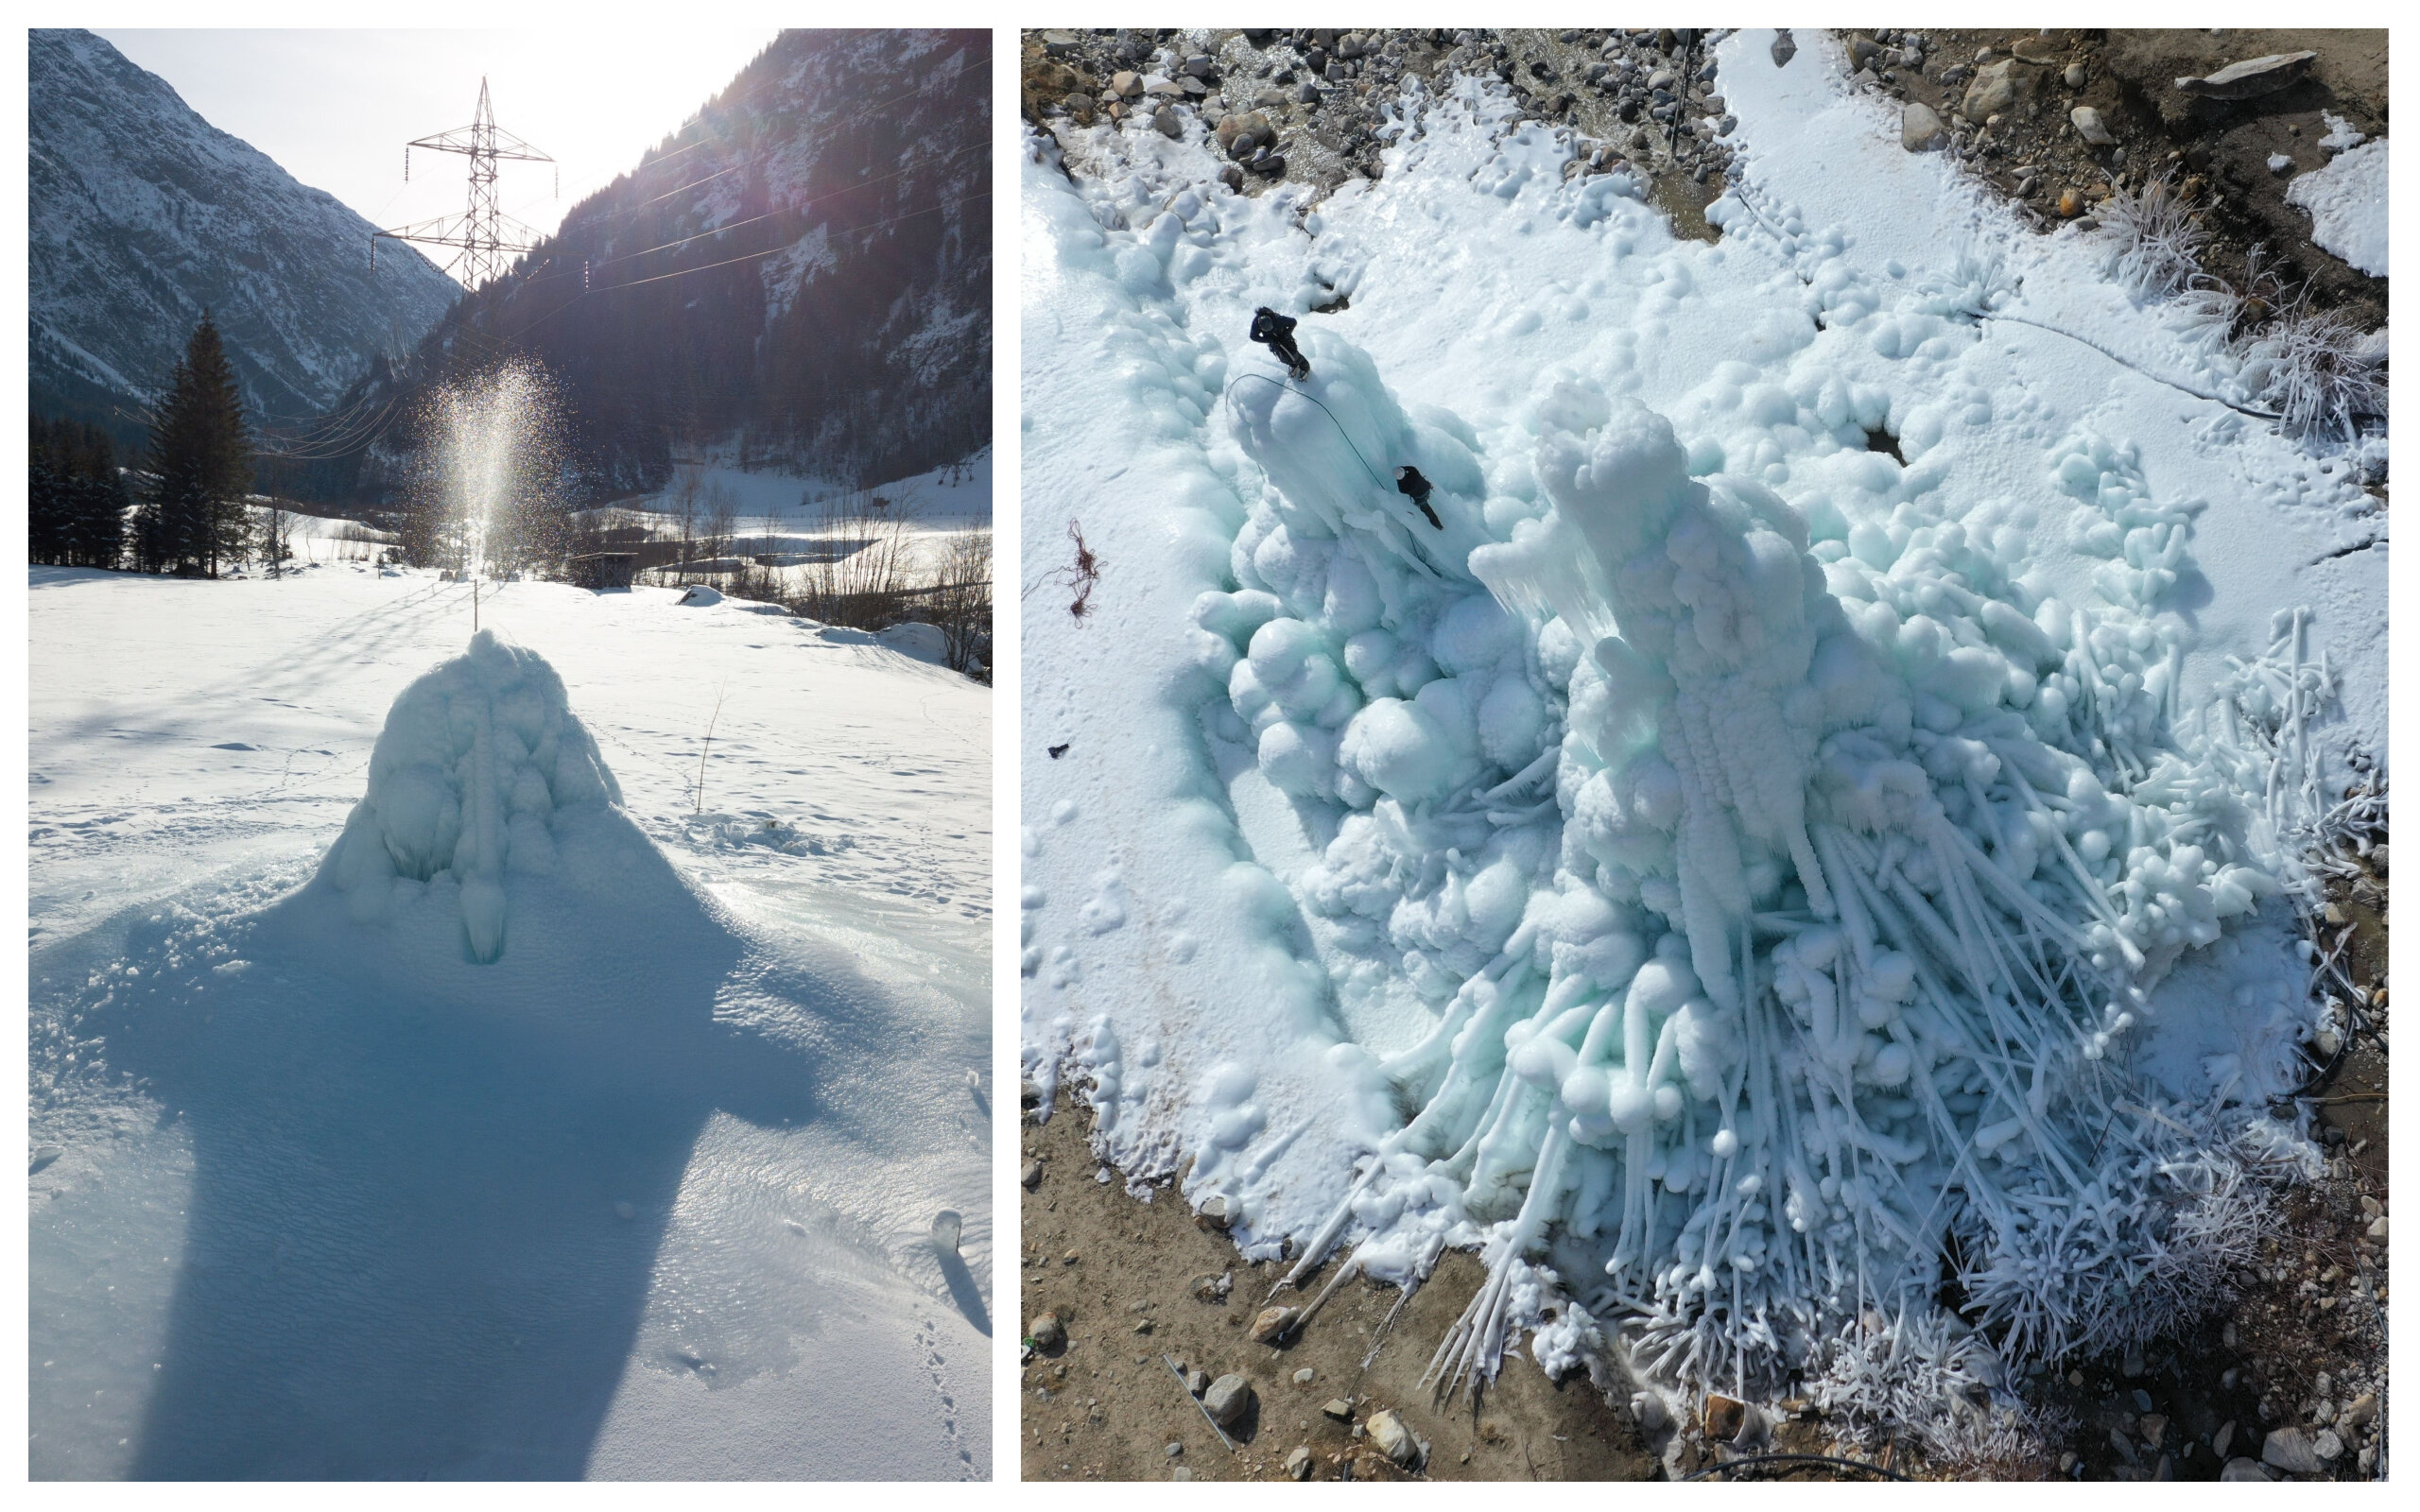
\includegraphics[width=12 cm]{figs/2AIRs.jpg}
%   \caption{The Swiss and Indian AIRs were 5 $m$ and 13 $m$ tall on January 9 and March 3, 2021 respectively. Picture
% credits: Daniel Bürki (left) and Thinles Norboo (right)} 
% \label{fig:2AIRs} 

% \end{figure}

\subsection{Meteorological data}

Air temperature, relative humidity, wind speed, pressure, longwave and global shortwave radiation are required
to calculate the surface energy balance of an AIR.  The resulting dataset highlights the difference in
meteorological influences driving ice volume evolution in the two study sites (see Table
\ref{tab:Observations}).

\begin{table}
  \centering
  \caption{Summary of the weather observations for AIRs built during the repective study period. 
The weather measurements are shown using their mean ($\mu$) and standard deviation ($\sigma$) during the study
period as $\mu \pm \sigma$. }

	\label{tab:Observations}
	\begin{tabular}{|lllll|}
		\textbf{Name}               & \textbf{Symbol} & \textbf{IN21} & \textbf{CH21} & \textbf{Units}   \\ 
		Air temperature             & $T_a    $       & $0 \pm 7$     & $2 \pm 6$     & $\degree C$      \\
		Relative humidity           & $RH     $       & $35 \pm 20$   & $79 \pm 18$   & \%               \\
    Wind speed                  & $v_a        $   & $3 \pm 1$     & $2 \pm 2$     & $m/s$            \\
		Direct Shortwave            & $SW_{direct} $  & $246 \pm 333$ & $80 \pm 156$  & $W\,m^{-2}$      \\
		Diffuse Shortwave           & $SW_{diffuse}$  & $0 \pm 0$     & $58 \pm 87$   & $W\,m^{-2}$      \\
		Hourly Precipitation        & $ppt        $   & $0 \pm 0$     & $139 \pm 457$ & $mm$             \\
		Pressure                    & $p_a         $  & $623 \pm 3$   & $794 \pm 9$   & $hPa$            \\
	\end{tabular}
\end{table}

\subsection{Fountain observations}

The fountain consists of a pipeline and a nozzle. The pipeline has three attributes, namely : discharge rate
($Q$), height ($h$) and water temperature ($T_F$). Discharge rate represents the discharge rate of the water in
the fountain pipeline. Height denotes the height of the fountain pipeline installed. Fountain water temperature
is the temperature of water droplets produced by the fountain.

The fountain nozzle has three characteristics, namely : the aperture diameter ($dia$) and pressure loss
($P_{nozzle}$) . Pressure loss denotes the loss of water head caused due to the fountain nozzle. Additionally,
the observed ice radius formed from the fountain water droplets is denoted as spray radius ($r_F$). 

\subsection{Drone flights}

\begin{table}
  \centering
  \caption{List of all the studied AIRs. The study period starts when the fountain was first switched on
  (denoted as Start Date) and ends when the respective AIR either melted or broke into several ice blocks
(denoted as Expiry Date). }

	\label{tab:AIRs}
	\begin{tabular}{|lllll|}
		\textbf{Name}     & \textbf{Start Date} & \textbf{Expiry Date} & \textbf{No. of flights} & \textbf{Spray radius} \\
    Traditional CH20  &  & & 2 & \\
    Traditional CH21  & Nov 22 2020   & May 10 2021 & 8 & 6.9 $m$ \\
    Traditional IN21  & Jan 18 2021   & June 20 2021 & 6 & 10.2 $m$ \\
    Traditional CH22  & Dec 8 2021 & April 12 2022 & 8 & \\
		Automated CH22  &  Dec 8 2021 & April 12 2022 & 6 & \\
	\end{tabular}
\end{table}

Several photogrammetric surveys were conducted for each of the AIRs. The details of these surveys and the
methodology used to produce the corresponding outputs are explained in paper I. The digital elevation models
(DEMs) generated from the obtained imagery were analysed to document the ice radius, the surface area and the
volume of the ice structures. Ice radius measurements of drone flights which observed either an increase in AIR
circumference or volume were averaged to determine the fountain's spray radius. The number of drone surveys
conducted for each of the AIRs and the corresponding spray radius observed is shown in Table \ref{tab:AIRs}. 

\section{AIR Model}

A bulk energy and mass balance model is used to calculate the amounts of ice, meltwater, water vapour and
wastewater of the AIR. In each hourly time step, the model uses the AIR surface area, energy balance and mass
balance calculations to estimate its ice volume, surface temperature and wastewater as shown in Fig.
\ref{fig:schema}.

% \begin{figure}
% 	\begin{center}
% 		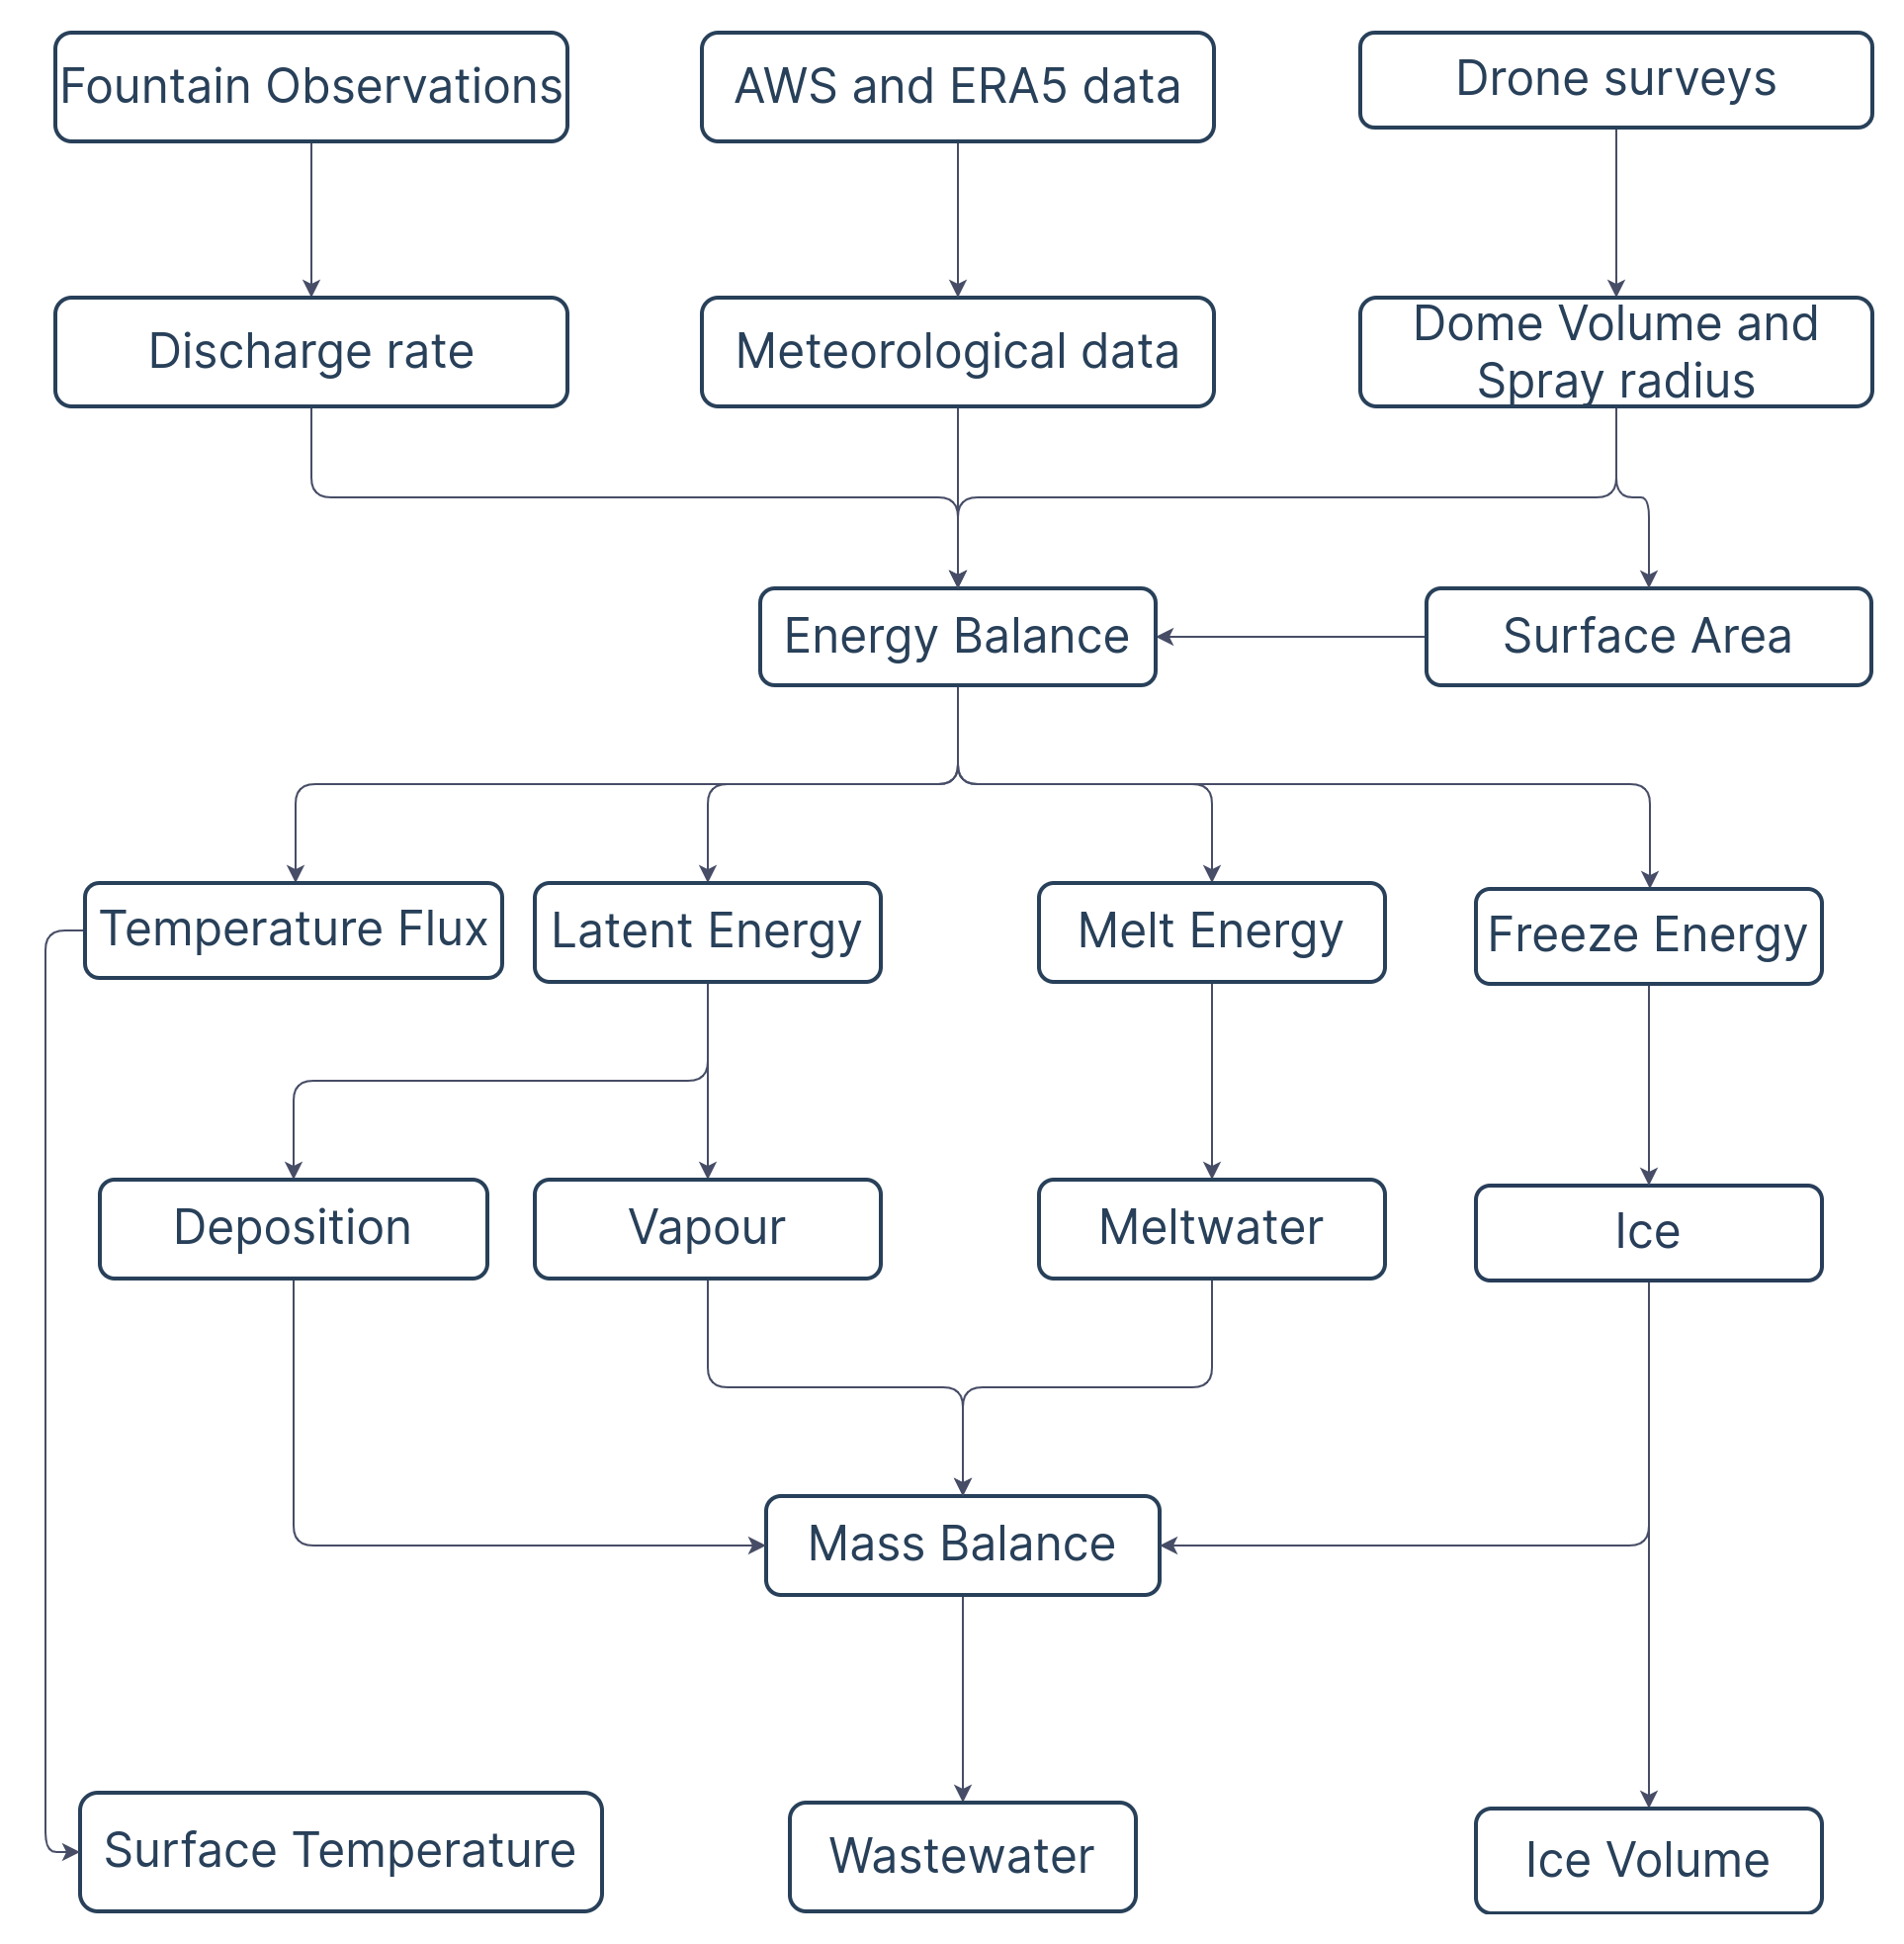
\includegraphics[width=10 cm]{figs/Figure_3.jpg}
% 	\end{center}
% 	\caption{Model schematic showing the workflow used in the model at every time step. }
% 	\label{fig:schema}
% \end{figure}

\subsection{Surface area calculation} \label{sec:shape}

The model assumes the AIR shape to be a cone and assigns the following shape attributes:

\begin{subequations}
	\begin{align}
		\label{eq:A}
		A_{cone}^i & = \pi \cdot r_{cone}^i \cdot \sqrt{{(r_{cone}^i)}^2 + {(h_{cone}^i})^ 2} \\
		\label{eq:V}
		V_{cone}^i & = \pi/3 \cdot {(r_{cone}^i)}^2 \cdot h_{cone}^i                                         \\
		\label{eq:thickness}
		j_{cone}^i & =\frac{\Delta M_{ice}^i}{\rho_{water}* A_{cone}^i}
	\end{align}
\end{subequations}

where $i$ denotes the model time step, $r_{cone}^i$ is the radius; $h_{cone}^i$ is the height; $A_{cone}^i$ is
the surface area; $V_{cone}^i$ is the volume and $j_{cone}^i$ is the AIR surface normal thickness change as shown
in Fig. \ref{fig:shape}. $M_{ice}^i$ is the mass of the AIR and $\Delta M_{ice}^i = M_{ice}^{i-1} -
M_{ice}^{i-2}$. Henceforth, the equations used display the model time step superscript $i$ only if it is different
from the current time step.

AIR density can be defined as:

\begin{equation}
  \rho_{cone} = \frac{M_{F} + M_{dep} + M_{ppt}}{(M_{F} + M_{dep})/\rho_{ice} + M_{ppt}/\rho_{snow}}
\end{equation}

where $M_F$ is the cumulative mass of the fountain discharge; $M_{ppt}$ is the cumulative precipitation;
$M_{dep}$ is the cumulative accumulation through water vapour deposition; $\rho_{ice}$ is the ice density (917
$kg\,m^{-3}$) and $\rho_{snow}$ is the density of wet snow (300 $kg\,m^{-3}$) taken from
\cite{cuffeyPhysicsGlaciers2010} .

AIR volume can also be expressed as:

\begin{equation} V_{cone} =\frac{M_{ice}} {\rho_{cone}} \label{eq:V1} \end{equation}

The initial radius of the AIR is assumed to be $r_F$. The initial height $h_0$ depends on the dome volume
$V_{dome}$ used to construct the AIR as follows:

\begin{equation}
	h_{0} =  \Delta x + \frac{3 \cdot V_{dome}}{\pi \cdot (r_F)^2 }
	\label{eq:h0}
\end{equation}

where $\Delta x$ is the surface layer thickness (defined in Section \ref{sec:energy})

During the subsequent time steps, the dimensions of the AIR evolve assuming a uniform thickness change ($j_{cone}$)
across its surface area with an invariant slope $s_{cone} = \frac{h_{cone}}{r_{cone}}$ .  During these time
steps, the volume is parameterised using Eqn. \ref{eq:V} as:

\begin{equation} V_{cone} = \frac{\pi \cdot {(r_{cone})}^3
		\cdot s_{cone}}{3} \label{eq:V2} \end{equation}

We define the Icestupa boundary through its spray radius, i.e. we assume ice formation is negligible when $r_{cone} >
	r_{F}$. Combining Eqns. \ref{eq:V},  \ref{eq:V1}, \ref{eq:h0} and \ref{eq:V2}, the geometric evolution of the
Icestupa at each time step $i$ can be determined by considering the following rules:

\begin{equation} (r_{cone},\, h_{cone}) = \left\{ \begin{array}{ll} (r_F ,\, h_0)                                                                          & \textit{ if } i=0 \\
		(r_{cone}^{i-1},\, \frac{3 \cdot M_{ice}}{\pi \cdot \rho_{ice} \cdot {(r_{cone}^{i-1})}^2}) & \textit{ if }
		r_{cone}^{i-1} \geq r_{F} \textit{ and } \Delta M_{ice} > 0                                                     \\ (\frac{3 \cdot M_{ice}}{\pi \cdot \rho_{ice} \cdot s_{cone}})^{1/3} \cdot (1,\,  s_{cone}) &
		otherwise\end{array} \right.  \label{eq:A2} \end{equation}


\subsection{Energy balance calculation} \label{sec:energy}

% \begin{figure}
% 	\begin{center}
% 		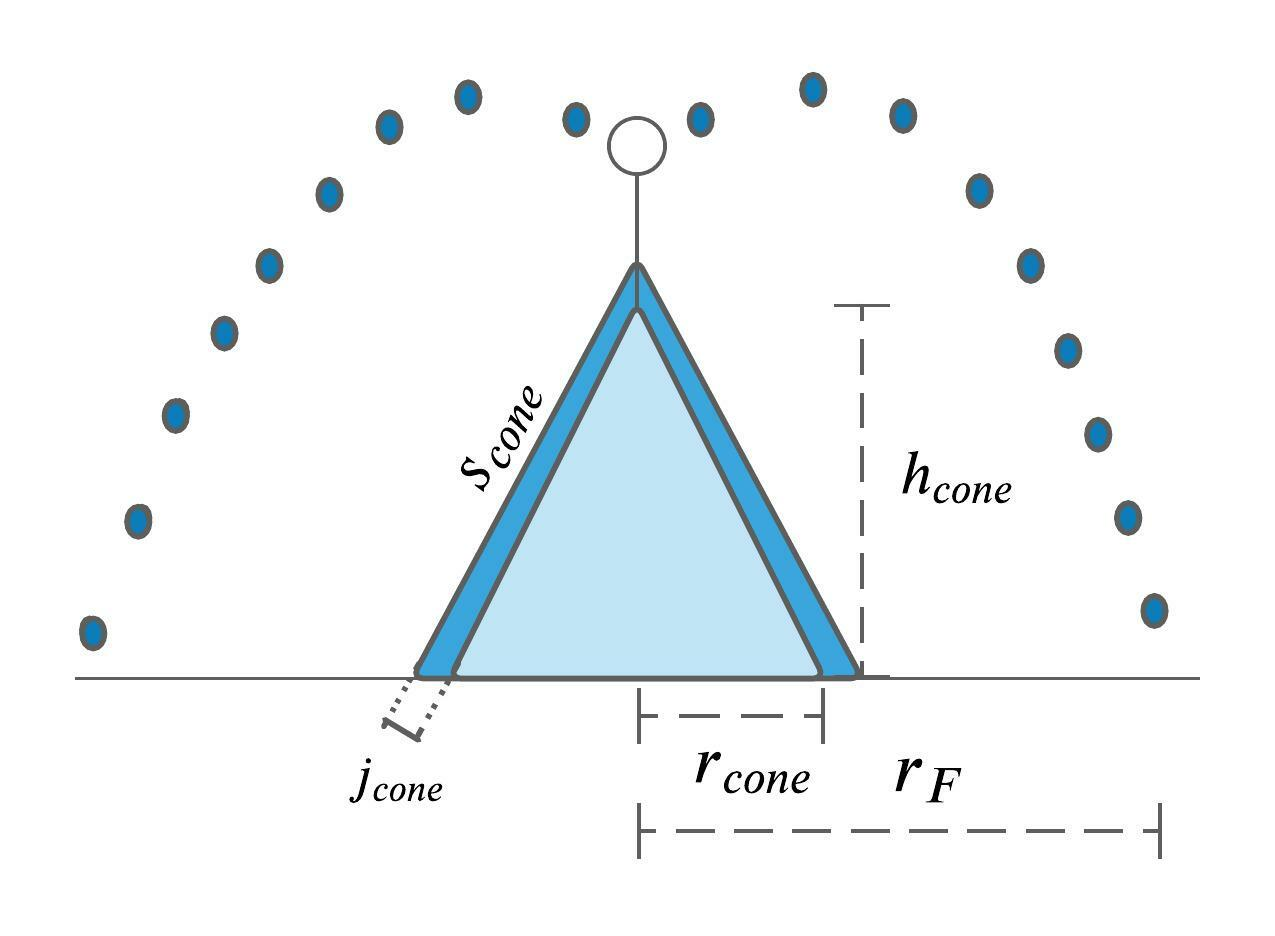
\includegraphics[width=10 cm]{figs/Figure_4.jpeg}
% 	\end{center}
% 	\caption{Shape variables of the AIR. $r_{cone}$ is the radius, $h_{cone}$ is the height, $j_{cone}$ is the
% 		thickness change and $s_{cone}$ is the slope of the ice cone. $r_F$ is the spray radius of the fountain.}
% 	\label{fig:shape}
% \end{figure}

We approximate the energy balance at the surface of an AIR by a one-dimensional description of energy fluxes
into and out of a (thin) layer with thickness $\Delta x$:

\begin{equation}
  \rho_{cone} \cdot c_{ice} \cdot \frac{\Delta T}{\Delta t} \cdot \Delta x = q_{SW} + q_{LW} + q_{L} + q_{S} + q_{F}+ q_{R} + q_{G}
	\label{eqn:EB}
\end{equation}

Upward and downward fluxes relative to the ice surface are positive and negative, respectively. The first term
is the energy change of the surface layer, which can be translated into a phase change energy should phase
changes occur. $q_{SW}$ is the net shortwave radiation; $q_{LW}$ is the net longwave radiation; $q_{L}$ and
$q_{S}$ are the turbulent latent and sensible heat fluxes. $q_{F}$ and $q_{R}$ represent the heat exchange of
the fountain water droplets and rain droplets with the AIR ice surface respectively. $q_{G}$ represents ground
heat flux between the AIR surface and its interior.

The density of the AIR $\rho_{cone}$ was parameterised as follows:

\begin{equation}
  \rho_{cone} = \frac{M_{F} + M_{dep} + M_{ppt}}{(M_{F} + M_{dep})/\rho_{ice} + M_{ppt}/\rho_{snow}}
\end{equation}

where $M_F$ is the cumulative mass of the fountain discharge; $M_{ppt}$ is the cumulative precipitation;
$M_{dep}$ is the cumulative accumulation through water vapour deposition; $\rho_{ice}$ is the ice density (917
$kg\,m^{-3}$) and $\rho_{snow}$ is the density of wet snow (300 $kg\,m^{-3}$) taken from
\cite{cuffeyPhysicsGlaciers2010} .

The energy flux acts upon the AIR surface layer, which has an upper and lower boundary defined by the atmosphere
and the ice body of the AIR, respectively. Here, we define the surface temperature $T_{ice}$ to be the modelled
average temperature of the icestupa surface layer.

\subsubsection{Net Shortwave Radiation \texorpdfstring{$q_{SW}$}{Lg}} \label{sec:SW}

The net shortwave radiation $q_{SW}$ is computed as follows:

\begin{equation} q_{SW} = (1- \alpha)\cdot (SW_{direct} \cdot f_{cone} + SW_{diffuse}) \label{eqn:SW} \end{equation}

where $SW_{direct}$ and $SW_{diffuse}$ are the direct and diffuse shortwave radiation, $\alpha$ is the
modelled albedo and $f_{cone}$ is the area fraction of the ice structure exposed to the direct shortwave
radiation.

The albedo varies depending on the water source that formed the current AIR surface layer. During the fountain
runtime, the albedo assumes a constant value corresponding to ice albedo. However, after the fountain is
switched off, the albedo can reset to snow albedo during snowfall events and then decay back to ice albedo. We
use the scheme described in \cite{oerlemansYearRecordGlobal1998} to model this process. The scheme records the
decay of albedo with time after fresh snow is deposited on the surface. $\delta t$ records the number of time
steps after the last snowfall event. After snowfall, albedo changes over a time step, $\delta t$ , as

\begin{equation} \alpha=\alpha_{ice}+(\alpha_{snow}-\alpha_{ice}) \cdot e^{(-\delta t)/\tau} \label{eqn:a}
\end{equation}

where $\alpha_{ice}$ is the bare ice albedo value (0.25), $\alpha_{snow}$ is the fresh snow albedo value (0.85)
and $\tau$ is a decay rate (16 $days$), which determines how fast the albedo of the ageing snow recedes back to
ice albedo. Discharge events decrease the decay rate by a factor of $\alpha_{ice}/\alpha_{snow}$. 

The solar area fraction $f_{cone}$ of the ice structure exposed to the direct shortwave radiation depends on the shape
considered. Using the solar elevation angle $\theta_{sun}$, the solar beam can be considered to have a vertical
component, impinging on the horizontal surface (semicircular base of the AIR), and a horizontal component
impinging on the vertical cross section (a triangle). The solar elevation angle $\theta_{sun}$ used is modelled
using the parametrisation proposed by \cite{woolfComputationSolarElevation1968}. Accordingly, $f_{cone}$ is determined as follows:

\begin{equation}
	\begin{split}
		f_{cone}& =\frac{(0.5 \cdot r_{cone} \cdot h_{cone}) \cdot cos \theta_{sun} +(\pi \cdot
			{(r_{cone})}^2/2) \cdot sin \theta_{sun} }{\pi \cdot r_{cone} \cdot ({(r_{cone})}^2+{(h_{cone})}^2)^{1/2}}\\
	\end{split}
	\label{eqn:f_{cone} }
\end{equation}

The diffuse shortwave radiation is assumed to impact the conical AIR surface uniformly.

\subsubsection{Net Longwave Radiation \texorpdfstring{$q_{LW}$}{Lg}} \label{sec:LW}

The net longwave radiation $q_{LW}$ is determined as follows:

\begin{equation}
	q_{LW}= LW_{in}-\sigma \cdot \epsilon_{ice} \cdot {(T_{ice}+ 273.15)}^4
	\label{eqn:LW}
\end{equation}

where $T_{ice}$ is the modelled surface temperature given in [$\degree C$],
$\sigma=5.67\cdot10^{-8}\,Jm^{-2}s^{-1}K^{-4}$ is the Stefan-Boltzmann constant, $LW_{in}$ denotes the incoming
longwave radiation and $\epsilon_{ice}$ is the corresponding emissivity value for the Icestupa surface (0.97).

The incoming longwave radiation $LW_{in}$ for the Indian site, where no direct measurements were available, is
determined as follows:

\begin{equation}
	LW_{in}=\sigma \cdot \epsilon_a \cdot {(T_a+ 273.15)}^4
	\label{eqn:LWin}
\end{equation}

here $T_a$ represents the measured air temperature and $\epsilon_a$ denotes the atmospheric emissivity. We
approximate the atmospheric emissivity $\epsilon_a$ using the equation suggested by \cite{brutsaertEvaporationAtmosphereTheory1982},
considering air temperature and vapor pressure (Eqn.  \ref{eqn:atm_e}). The vapor pressure of air over water and
ice was obtained using Eqn. \ref{eqn:vp}.  The expression defined in \cite{brutsaertDerivableFormulaLongwave1975} for clear skies
(first term in equation \ref{eqn:atm_e}) is extended with the correction for cloudy skies after
\cite{brutsaertEvaporationAtmosphereTheory1982} as follows:

\begin{equation}
	\epsilon_a=1.24 \cdot (\frac{p_{v,w}}{(T_a+273.15)})^{1/7}\cdot(1+0.22\cdot{cld}^2) \label{eqn:atm_e}
\end{equation}

with a cloudiness index $cld$, ranging from 0 for clear skies to 1 for complete overcast skies. For the Indian
site, we assume cloudiness to be negligible.

\subsubsection{Turbulent fluxes} \label{sec:Qs}

The turbulent sensible $q_{S}$ and latent heat $q_{L}$ fluxes are computed with the following expressions
proposed by \cite{garrattAtmosphericBoundaryLayer1992}:

\begin{equation}
	q_{S}=\mu_{cone}\cdot c_{a} \cdot \rho_{a} \cdot p_{a}/p_{0,a} \cdot \frac{\kappa^2 \cdot v_a \cdot
		(T_a-T_{ice})}{{(\ln{\frac{h_{AWS}}{z_{0}}})}^2}
	\label{eqn:qs}
\end{equation}

\begin{equation}
	q_{L}=\mu_{cone}\cdot 0.623 \cdot L_s \cdot \rho_{a}/p_{0,a} \cdot \frac{\kappa^2 \cdot
	v_a(p_{v,w}-p_{v,ice})}{{(\ln{\frac{h_{AWS}}{z_{0}}})}^2}
\end{equation}

where $h_{AWS}$ is the measurement height above the ground surface of the AWS (around $2\,m$ for all sites),
$v_a$ is the wind speed in [$m\,s^{-1}$], $c_a$ is the specific heat of air at constant pressure (1010 J
$kg^{-1} K^{-1}$), $\rho_{a}$ is the air density at standard sea level (1.29 $kg m^{-3}$), $p_{0,a}$ is the air
pressure at standard sea level (1013 $hPa$), $p_{a}$ is the measured air pressure, $\kappa$ is the von Karman
constant (0.4), $z_{0}$ is the surface roughness (3 $mm$) and $L_s$ is the heat of sublimation (2848
$kJ\,kg^{-1}$).  The vapor pressure of air with respect to water ($p_{v,w}$) and with respect to ice
($p_{v,ice}$) was obtained using the formulation given in \cite{huangSimpleAccurateFormula2018} :

\begin{equation}
	\begin{split}
		p_{v,w}&=e^{\frac{(34.494 - \frac{4924.99}{T_{a} + 237.1})}{(T_a + 105)^{1.57} \cdot 100}} \cdot \frac{RH}{100} \\
		p_{v,ice}&=e^{\frac{(43.494 - \frac{6545.89}{T_{ice} + 278})}{(T_{ice} + 868)^{2} \cdot 100}} \\
	\end{split} \label{eqn:vp}
\end{equation}

The dimensionless parameter $\mu_{cone}$ is an exposure parameter that deals with the fact that AIR has a rough
appearance and forms an obstacle to the wind regime. This factor accounts for the larger turbulent fluxes due to
the roughness of the surface \citep{oerlemansBriefCommunicationGrowth2021}, and is a function of the AIR slope
as follows:

\begin{equation}
	\mu_{cone} = 1 + \frac{s_{cone}}{2}
\end{equation}

A possible source of error is the fact that wind measurements from the horizontal plane at the AWS are used,
which might be different from those on a slope. However, without detailed datasets from the AIR surface, we
retain this assumption.

\subsubsection{Fountain discharge heat flux \texorpdfstring{$q_{F}$}{Lg} } \label{sec:heatflux}

The fountain water temperature $T_F$ is assumed to cool to 0 $\degree C$ after contact with the ice surface.
$T_F$ is equal to the measured source water temperature. But during time periods when the ambient temperature is
subzero, $T_F$ is assumed to be 0 $\degree C$. Thus, the heat flux caused by this process is:

\begin{equation}
	q_{F} = \left\{ \begin{array}{ll}
		\frac{ \Delta M_F \cdot c_{water} \cdot T_F}{\Delta t \cdot A_{cone}} & \textit{ if } T_{temp} > 0 \\
		0   & \textit{ otherwise}
	\end{array} \right.
\end{equation}

with $c_{water}$ as the specific heat of water (4186 J $kg^{-1} K^{-1}$).

\subsubsection{Rain heat flux \texorpdfstring{$q_{R}$}{Lg} }

The influence of rain events on the albedo and the energy balance was assumed to be similar to that of discharge
events. However, the water temperature of a rain event was assumed to equal to the air temeperature. Accordingly,
the heat flux generated due to a rain event was equal to:

\begin{equation}
  q_{R} = \frac{ \Delta M_{ppt} \cdot c_{water} \cdot T_a}{\Delta t \cdot A_{cone}}
	\label{eqn:qR}
\end{equation}

\subsubsection{Bulk Icestupa heat flux \texorpdfstring{$q_{G}$}{Lg}} \label{sec:Bulkflux}

The bulk Icestupa heat flux $q_{G}$ corresponds to the ground heat flux in normal soils and is caused by the
temperature gradient between the surface layer ($T_{ice}$) and the ice body ($T_{bulk}$). It is expressed by
using the heat conduction equation as follows:

\begin{equation} q_{G} = k_{ice} \cdot (T_{bulk}-T_{ice}^{i-1})/l_{cone} \label{eqn:qG}    \end{equation}

where $k_{ice}$ is the thermal conductivity of ice (2.123 $W\, m^{-1}\,K^{-1}$) , $T_{bulk}$ is the mean
temperature of the ice body within the icestupa and $l_{cone}$ is the average distance of any point in the
surface to any other point in the ice body. $T_{bulk}$ is initialised as 0 $\degree C$ and later determined from
Eqn. \ref{eqn:qG} as follows:

\begin{equation} T_{bulk}^{i+1} = T_{bulk} - (q_{G} \cdot A \cdot \Delta t)/(M_{ice} \cdot c_{ice}) \end{equation}

Since AIRs typically have conical shapes with $r_{cone} > h_{cone}$, we assume that the center of mass of the cone
body is near the base of the fountain. Thus, the distance of every point in the AIR surface layer from the cone
body's center of mass is between $h_{cone}$ and $r_{cone}$. Therefore, we calculate $q_{G}$ assuming $l_{cone} = (r_{cone} +
	h_{cone})/2$.

\subsubsection{Phase changes}\label{sec:phase}

In this section, the numerical procedures to model phase changes at the surface layer are explained. Let
$T_{temp}$ be the calculated surface temperature. Therefore, Eqn. \ref{eqn:EB} can be rewritten as:

$$q_{total} =\rho_{ice} \cdot c_{ice} \cdot \frac{(T_{temp}-T_{ice})}{\Delta t} \cdot \Delta x$$

where $q_{total}$ represents the total energy available to be redistributed. Even if the numerical heat transfer
solution produces temperatures which are $T_{temp}>0\, \degree C$, say from intense shortwave radiation, the ice
temperature must remain at $T_{temp} = 0\, \degree C$. The ‘‘excess’’ energy is used to drive the melting
process. Moreover, the energy input is used to melt the surface ice layer, and not to raise the surface
temperature to some unphysical value. Similarly, for freezing to occur, three conditions are required. Firstly,
fountain water is present ($\Delta M_{F} > 0 $) and secondly the calculated temperature of the ice, $T_{temp}$,
is below $0\, \degree C$. However, these two conditions are not sufficient as the latent heat turbulent fluxes
can only contribute to temperature fluctuations. Therefore, an additional condition, namely, $(q_{total}-q_{L})
< 0$, is required. Depending on the above conditions, the total energy $q_{total}$ can be redistributed
for the melting ($q_{melt}$), freezing ($q_{freeze}$) and surface temperature change ($q_{T}$) processes as
follows:

\begin{equation}
	q_{total} = \left\{ \begin{array}{ll}
		q_{freeze} + q_{T} & \textit{ if } \Delta M_{F} > 0 \textit{ and } T_{temp} < 0 \textit{ and }(q_{total}-q_{L}) < 0 \\
		q_{melt} + q_{T}   & \textit{ otherwise}
	\end{array} \right.
\end{equation}

Henceforth, time steps when the the total energy is redistributed to the freezing energy are called freezing
events and the rest of the time steps are called melting events.


During a freezing event, the AIR surface is assumed to warm to $0 \degree C$. The available energy
$(q_{total}-q_{L})$ is further increased due to this change in surface temperature represented by the energy
flux:

$$q_{0} = \frac{\rho_{ice} \cdot \Delta x \cdot c_{ice} \cdot T_{ice}^{i-1}}{\Delta t}$$

The available fountain discharge ($\Delta M_{F}$) may not be sufficient to utilize all the freezing energy. At such times, 
the additional freezing energy further cools down the surface temperature. Accordingly, the surface energy flux
distribution during a freezing event can be represented as:

\begin{equation}
	(q_{freeze}, q_{T}) = \left\{ \begin{array}{ll}
		(\frac{\Delta M_{F} \cdot L_f
		}{A_{cone} \cdot \Delta t}
		, q_{total}+\frac{\Delta M_{F} \cdot L_f
		}{A_{cone} \cdot \Delta t})          & \textit{ if  } \Delta M_{F} \textit{ insufficient }\\
		(q_{total}-q_{L}+q_{0}, q_{L}-q_{0}) & \textit{ otherwise }                                                                      \\
	\end{array} \right.
\end{equation}

If $T_{temp} > 0 \degree C$, then energy is reallocated from $q_{T}$ to $q_{melt}$ to maintain surface
temperature at melting point. The total energy flux distribution during a melting event can be represented as:

\begin{equation}
	(q_{melt}, q_{T}) = \left\{ \begin{array}{ll}
		(0, q_{total})
    & \textit{ if } T_{temp} \leq 0 \\
		(\frac{T_{temp} \cdot \rho_{ice} \cdot c_{ice} \cdot \Delta x}{\Delta t}, q_{total}-\frac{T_{temp} \cdot \rho_{ice} \cdot c_{ice} \cdot \Delta x}{\Delta t}  ) & \textit{ if } T_{temp} > 0
	\end{array} \right.
\end{equation}


\subsection{Mass balance calculation}

The mass balance equation for an AIR is represented as:

\begin{equation}
	\frac{\Delta M_{F} + \Delta M_{ppt} + \Delta M_{dep}}{\Delta t} = \frac{\Delta M_{ice} +\Delta M_{water} +
		\Delta M_{sub} + \Delta M_{waste}}{\Delta t}  \\
	\label{eq:MB}
\end{equation}

where $M_{F}$ is the cumulative mass of the fountain discharge; $M_{ppt}$ is the cumulative precipitation;  $M_{dep}$ is the cumulative
accumulation through water vapour deposition; $M_{ice}$ is the cumulative mass of ice; $M_{water}$ is the cumulative
mass of melt water; $M_{sub}$ represents the cumulative water vapor loss by sublimation and $M_{waste}$ represents the
fountain wastewater that did not interact with the AIR. The left hand side of equation \ref{eq:MB} represents the rate of
mass input and the right hand side represents the rate of mass output for an AIR.

Precipitation input is calculated as shown in equation \ref{eq:ppt} where $\rho_{w}$ is the density of water (1000
$kg\,m^{-3}$), $\Delta ppt/ \Delta t$ is the measured precipitation rate in [$m\,s^{-1}$] and $T_{ppt}$ is the temperature threshold
below which precipitation falls as snow. Here, snowfall events were identified using $T_{ppt}$ as $1 \degree C$. Snow
mass input is calculated by assuming a uniform deposition over the entire circular footprint of the AIR.

The latent heat flux is used to estimate either the evaporation and condensation processes or sublimation and deposition
processes as shown in equation \ref{eq:vap}. During the time steps at which the surface temperature is below 0 $\degree C$ only
sublimation and deposition can occur, but if the surface temperature reaches 0 $\degree C$, evaporation and condensation
can also occur. As the differentiation between evaporation and sublimation (and condensation and deposition) when the
air temperature reaches 0 $\degree C$ is challenging, we assume that negative (positive) latent heat fluxes correspond
only to sublimation (deposition), i.e. no evaporation (condensation) is calculated.

Since we have categorized every time step as a freezing or melting event, we can determine the melting/freezing
rates and the corresponding meltwater/ice quantities as shown in equations \ref{eq:m_freeze/melt}, \ref{eq:mwat}
and \ref{eq:mcone}. Having calculated all other mass components, the fountain wastewater generated every
time step can be calculated using Eqn. \ref{eq:MB}.

\begin{subequations}
	\begin{align}
		\frac{\Delta M_{F}}{\Delta t} & = \left\{ \begin{array}{ll} \frac{60}{\rho_w \cdot \Delta t} \cdot d_F
			 & \textit{ if fountain is on} \\ 0 & \textit{ otherwise } \\\end{array} \right.                                             \\
		\label{eq:ppt}
		\frac{\Delta M_{ppt}}{\Delta t}                                    & = \left\{ \begin{array}{ll} \pi \cdot
        {(r_{cone})}^2 \cdot
			\rho_{w}\cdot \frac {\Delta ppt}{\Delta t} & \textit{ if } T_{a} < T_{ppt} \\ 0 & \textit{ if } T_{a} \geq T_{ppt} \\\end{array} \right.                                             \\
		\label{eq:vap}
		(\frac{\Delta M_{dep}}{\Delta t}, \frac{\Delta M_{sub}}{\Delta t}) & = \left\{ \begin{array}{ll} \frac{q_{L}
			\cdot A_{cone}}{L_s}\cdot (1,0)  & \textit{ if } q_{L} \geq 0 \\ \frac{q_{L}
			\cdot A_{cone}}{L_s}\cdot (0,-1) & \textit{ if } q_{L} < 0    \\\end{array} \right.                                             \\
		\label{eq:mwat}
		\frac{\Delta M_{water}}{\Delta t}                                  & = \frac{q_{melt} \cdot A_{cone} }{L_f}                                                   \\
	  \label{eq:m_freeze/melt}
    \frac{\Delta M_{freeze/melt}}{\Delta t} & = \frac{q_{freeze/melt} \cdot A_{cone} }{L_f} \\
		\label{eq:mcone}
		\frac{\Delta M_{ice}}{\Delta t}                                    & = \frac{q_{freeze}\cdot A_{cone} }{L_f} + \frac{\Delta M_{ppt}}{\Delta t} + \frac{\Delta
			M_{dep}}{\Delta t}- \frac{\Delta M_{sub}}{\Delta t}- \frac{\Delta M_{water}}{\Delta t}
	\end{align}
\end{subequations}

Considering AIRs as water reservoirs, their net water loss can be defined as:

\begin{equation} \textit{Net water losses} = \frac{M_{waste}+M_{sub}}{(M_F+M_{ppt}+M_{dep})} \cdot 100 \end{equation}


\subsection{Uncertainty Quantification}

The uncertainty in the model of estimating ice volumes is caused by three sources, namely, model forcing
data, model hyperparameters and model parameters. Model forcing data can further be divided into weather and
fountain forcing data. Significant uncertainty exists in the weather forcing data, particularly for all the
radiation measurements ($SW_{direct}, SW_{diffuse}, LW_{in}$) since they were taken from ERA5 dataset or an AWS
far away from the construction sites. Since no other weather datasets exist for comparison, especially near the
IN21 AIR, we are not accounting for uncertainties related to meteorological forcing data in this analysis.
Uncertainty in the fountain forcing data arises due to only some fountain parameters listed in Table
\ref{tab:parameters}. Fountain runtime $t_F$ has no uncertainty for the Swiss AIRs because no interruptions
occured during the study period. However, significant uncertainty exists for the IN21 AIR , where the
interruptions due to pipeline freezing events happened overnight but this was ignored in this analysis. Fountain
spray radius $r_F$ was measured using the drone survey and therefore also doesn't contribute to model
uncertainty. The choice of mean discharge rate $d_F$ for both sites was just a best guess, based on few observations made by the
flowmeter. So we associate this parameter by a large uncertainty of $\pm \,50\, \%$. For the fountain water
temperature $T_F$, we assumed an upper bound of $3\, \degree C$ since it is unlikely for it to have been beyond
this range considering winter conditions at all the sites. The model structure introduces uncertainty through
the spatial and temporal hyperparameters $\Delta x$ and $\Delta t$. By definition, $\Delta x$ is directly
proportional to $\Delta t$. Therefore, we fix the temporal resolution of the model at hourly timesteps and only
investigate the uncertainty caused by $\Delta x$ here. Since the surface layer thickness for an AIR does not
resemble to any parameter in the glaciological literature, we attribute a wide range of values for it (from 1 cm
to 10 cm). The model parameters are henceforth called as weather parameters to distinguish them from the
fountain forcing parameters. These were fixed within a range based on literature values (see Table
\ref{tab:parameters}). 

The three types of uncertain parameters namely, model hyperparameters ($\Delta x$), fountain forcing parameters
($d_F, T_F$) and weather parameters ($\epsilon_{ice}, z_0, \alpha_{ice}, \alpha_{snow}, T_{ppt}, \tau$) are
denoted as $Q^M, Q^F$ and $Q^W$ henceforth. Together, these nine parameters cause a large uncertainty in the ice
volume estimates. In order to reduce this uncertainty, we perform a global sensitivity analysis with the net
water loss as our objective. The objective of this sensitivity analysis was to reduce the dimension of the
parameter space by calibrating the parameters with high total-order sensitivities ($S_{T_{j}} > 0.5$). The
methodology to determine $S_{T_{j}}$ is described in Appendix \ref{sec:uncertainpy}. These sensitive model
parameters were calibrated based on the root mean squared error (RMSE) between the drone surveys (see Table
\ref{tab:uav}) and the model estimations of the ice volume. For this calibration procedure, all the other
parameters were set to the median value of their respective ranges defined in Table \ref{tab:parameters}.  The
sensitivity analysis and calibration were carried out with the drone surveys of CH21 and IN21 AIRs. 

The model uncertainty was quantified separately for the remaining parameters in $Q^M, Q^F$ and $Q^W$ using the
corresponding $90\, \%$ prediction interval $I^M, I^F$ and $I^W$. The $90\, \%$ prediction interval, $I^k$, gives us the
interval within which $90\,\%$ of the ice volume outcomes occur when all the parameters in $Q^k$ are varied
assuming each has an independent uniform probability density function. $5\,\%$ of the outcomes are above and
$5\,\%$ are below this interval. The methodology to obtain this is described in Appendix \ref{sec:uncertainpy}.

For validation, the calibrated model was tested with two datasets namely, the expiry date of all AIRs and the
drone surveys of CH20 AIR.

% \begin{table}
%   \caption{Free parameters in the model categorised as constant, derived, model hyperparameters, weather and
%   fountain forcing parameters with their respective values/ranges.}

% 	\label{tab:parameters}
% 	\begin{tabular}{lllll}
% 		\toprule
% 		\textbf{Constant Parameters}                       & \textbf{Symbol} & \textbf{Value} &
%     \textbf{Unit} & \textbf{References} \\
%     Van Karman constant & $\kappa$      & 0.4        &dimensionless & \citeauthor{CuffeyPaterson_2010}              \\
%     Stefan Boltzmann constant & $\sigma$ & $\num{5.67 e-8} $& $W\, m^{-2}\, K^{-4}$ & \citeauthor{CuffeyPaterson_2010}\\
%     Air pressure at sea level & $p_{0,a}$ & 1013 & $hPa$  & \citeauthor{MolgHardy_2004}\\
%     Density of water & $\rho_{w}$ & 1000 & $kg\, m^{-3}$    & \citeauthor{CuffeyPaterson_2010}\\
%     Density of ice & $\rho_{ice}$ & 917 & $kg\, m^{-3}$ & \citeauthor{CuffeyPaterson_2010}\\
%     Density of air & $\rho_{a}$ &  1.29 & $kg\, m^{-3}$   & \citeauthor{MolgHardy_2004}\\
%     Specific heat of water & $c_{w}$ & 4186 & $J\, kg^{-1}\,\degree C^{-1}$  & \citeauthor{CuffeyPaterson_2010}\\
%     Specific heat of ice & $c_{ice}$ & 2097 & $J\, kg^{-1}\,\degree C^{-1}$ & \citeauthor{CuffeyPaterson_2010}\\
%     Specific heat of air & $c_{a}$ & 1010 & $J\, kg^{-1}\,\degree C^{-1}$ & \citeauthor{MolgHardy_2004}\\
%     Thermal conductivity of ice & $k_{ice}$ & 2.123  & $W\, m^{-1}\, K^{-1}$ & \citeauthor{Bonales_2017} \\
%     Latent Heat of Sublimation & $L_{s}$ & \num{2.848e6}  & $J\, kg^{-1}$ &   \citeauthor{CuffeyPaterson_2010}\\
%     Latent Heat of Fusion & $L_{f}$ & \num{3.34e5} & $J\, kg^{-1}$ & \citeauthor{CuffeyPaterson_2010}\\
%     Gravitational acceleration & $g$ & 9.81 & $m\, s^{-2}$ &\citeauthor{CuffeyPaterson_2010}\\
%     Weather station height & $h_{AWS}$ & 2 & $m$ & assumed \\
%     Model timestep                            & $\Delta t$            & $3600$           & $s$ & assumed \\
%     Fountain spray radius & $r_{F}$             &             & $m$& measured \\
%     Fountain runtime & $t_{F}$             &             &  $hours$ & measured \\\midrule
% 		\textbf{Derived Parameters} & \textbf{Symbol} & \textbf{} & \textbf{Unit} & \textbf{Section} \\
%     Radius of AIR & $r_{cone}$ &  & $m$ & \ref{sec:shape}\\
%     Height of AIR & $h_{cone}$ &  & $m$ & \ref{sec:shape}\\
%     Slope of AIR  & $s_{cone}$ &  & dimensionless & \ref{sec:shape}\\
%     Thickness change of AIR  & $j_{cone}$ &  & $m$  & \ref{sec:shape}\\
%     Atmospheric emissivity & $\epsilon_{a}$ & & dimensionless    & \ref{sec:LW}\\
%     Cloudiness & $cld$ &  & dimensionless  & assumed\\
%     Vapour pressure over water & $p_{v,w}$ &  & $hPa$  & \ref{sec:Qs}\\
%     Vapour pressure over ice & $p_{v,ice}$ &  & $hPa$ & \ref{sec:Qs}\\
%     Solar elevation angle & $\theta_{sun}$ &  & $\degree$ & \ref{sec:SW}\\
%     Albedo & $\alpha$ &  & dimensionless & \ref{sec:SW}\\
%     Solar area fraction& $f_{cone}$ &  & dimensionless & \ref{sec:SW}\\
%     Ice body and surface distance & $l_{cone}$ &  & $m$  & \ref{sec:Bulkflux}\\
%     AIR surface temperature & $T_{ice}$ &  & $\degree C$  & \ref{sec:Bulkflux}\\
%     AIR bulk temperature & $T_{bulk}$ &  & $\degree C$  & \ref{sec:Bulkflux}\\\midrule
% 		\textbf{Model Hyperparameters} & \textbf{Symbol} & \textbf{Range} & \textbf{Unit} & \textbf{References} \\
%     Surface layer thickness             & $\Delta x$            & $[\num{1e-2},\num{1e-1}]$           & $m$ & assumed
%     \\\midrule
% 		\textbf{Weather Parameters} & \textbf{Symbol} & \textbf{Range} & \textbf{Unit} & \textbf{References} \\
%     Ice Emissivity                      & $\epsilon_{ice}$      & $[0.95,0.99]$         & dimensionless & \citeauthor{HORI2006486}             \\
%     Surface Roughness                   & $z_0$                 & $[\num{1e-3},\num{5e-3}]$            & $m$  & \citeauthor{BrockWillisSharp_2006}       \\
%     Ice Albedo                          & $\alpha_{ice}$        & $[0.15,0.35]$         & dimensionless  &
%     \citeauthor{steiner_2015};            \\
%     & &    &  & \citeauthor{ZollesMaussion_2019}      \\
%     Snow Albedo                         & $\alpha_{snow}$       & $[0.8,0.9]$        & dimensionless  & \citeauthor{ZollesMaussion_2019}              \\
%     Precipitation Temperature threshold & $T_{ppt}$             & $[0,2]$            & $\degree C$& \citeauthor{Zhou_2010}  \\
%     Albedo Decay Rate                   & $\tau$                & $[10,22]$           & $days$ &
%     \citeauthor{Schmidt_2017};      \\
%     & &    &  & \citeauthor{OerlemansKnap_1998}      \\\midrule
% 		\textbf{Fountain Forcing Parameters} & \textbf{Symbol} & \textbf{Range} & \textbf{Unit} & \textbf{References} \\
%     Discharge rate & $d_{F}$             & $[0.5 \cdot d_{F},1.5 \cdot d_{F}]$            & $l/min$& assumed  \\
%     Water temperature & $T_{F}$             & $[0,3]$            & $\degree C$  & assumed  \\\bottomrule
% 	\end{tabular}
% \end{table}

\section{Model application}

\subsection{Calibration of sensitive parameters}

The total-order sensitivities of all the nine parameters with respect to the net water loss objective are shown
in Fig. \ref{fig:param_hist} (a) . In total, the global sensitivity analysis required 1432 model runs to determine
these sensitivities for each site. The only sensitive parameter ($S_{T_{j}} > 0.5$) for both AIRs was the
surface layer thickness. The RMSE between the drone surveys and the model ice volume estimates for different
surface layer thickness are shown in Fig. \ref{fig:param_hist} (b). The optimum value of $\Delta x$ was found to
be 45 $mm$ and 65 $mm$ with an RMSE of 9 $m^3$ and 30 $m^3$ for CH21 and IN21 AIRs respectively.

% \begin{figure}
% 	\begin{center}
% 		\includegraphics[width=\linewidth]{Figures/Figure_5.jpg}
% 	\end{center}
%   \caption{(a) Total-order sensitivities of all the uncertain parameters of the model with net water loss as the
%   objective. (b) The calibration of the sensitive parameter, $\Delta x$ with the RMSE between the drone and
% model estimates of the ice volume. The dots denote the optimum values. The estimates from the Swiss and Indian
% AIRs are denoted with blue and red colors respectively. }
% 	\label{fig:param_hist}
% \end{figure}

\subsection{Weather and fountain forcing uncertainty quantification}

The uncertainty in the ice volume estimates caused by the weather and fountain forcing parameters are shown in
Fig. \ref{fig:results}. The ranges highlighted represent the corresponding $90\,\%$ prediction interval of the
ice volume estimates. Weather uncertainty determination required 422 simulations whereas fountain forcing
uncertainty determination required 32 simulations for each AIR. Since the results presented below differ
significantly during the fountain runtime, we divided the simulation duration of the AIR into accumulation and
ablation periods. The accumulation (ablation) period ends (starts) at the last fountain discharge event. 
 

The prediction interval of the weather and fountain forcing parameters behave differently during the
accumulation and ablation period for all AIRs. Prediction interval of the weather parameters increase
throughout the simulation period, but that of the fountain forcing parameters only increase during the
accumulation period. This is to be expected since the fountain forcing parameters directly affect the model
estimates only during the accumulation period. 

Weather uncertainty for the Indian site was low compared to the Swiss since precipitation and the associated
variation in albedo was negligible. At the end of the accumulation period, the Indian weather prediction
interval had a magnitude of  $73\,m^3$ which was 10 \% of the maximum simulated volume, whereas the magnitude of
the Swiss weather prediction interval was much higher (28 \% of the maximum simulated volume for the CH21 AIR).
This was expected since four out of the six uncertain Indian weather parameters were part of the albedo module. Among
all the weather parameters, surface roughness caused the most variance in both Indian and the Swiss ice
volume estimates.

Fountain forcing uncertainty for the Indian site was higher than its weather uncertainty (28 \% of the maximum
simulated volume at the end of the accumulation period). This was predominantly due to the uncertainty in the
fountain's water temperature. However, for the Swiss site, the prediction interval of the fountain forcing
parameters was similar to that of the weather parameters during the accumulation period. Since the mean fountain
discharge rate of the Indian location was eight times that of the Swiss, the uncertainty due to the fountain
forcing parameters was expected to be larger for the Indian location.

\subsection{Validation}

Model performance can be judged based on the ice volume left on the expiry date of all AIRs. In the case of CH21
AIR no ice volume was left whereas for CH20 AIR ice volume of 12 $m^3$ was left on the expiry date. For the IN21
AIR, the determination of the expiry date was not possible. In reality, the IN21 AIR was found to have
disintegrated into several ice blocks on 20th June, 2021. 

There was also one drone survey of the CH20 AIR volume for validation purposes (see Table \ref{tab:uav}). The
RMSE of that observation with the modelled volume was $19\, m^3$ which is 18 \% of the maximum simulated ice
volume of CH20 AIR.

% \begin{figure}
% 	\begin{center}
% 		\includegraphics[width=\linewidth]{Figures/Figure_6.jpg}
% 	\end{center}
% 	\caption{Simulated ice volume during the lifetime of the AIRs (blue curve). The shaded regions (light blue and
% 		orange) represent the 90\% prediction interval of the AIR ice volume caused by the variations in weather and
%     fountain forcing parameters, respectively. Violet points indicate the drone ice volume observations.  The grey
%   dashed line represents the observed expiry date for each AIR.  }
% 	\label{fig:results}
% \end{figure}

\section{Model extensions}

The AIR model presented above was extended in order to (a) develop automated fountain scheduling strategies and
(b) improve its transferability to new locations.

\subsection{Automated fountain scheduling system}

Recommended discharge rates can only be produced if more information about the AIR surface properties and
weather conditions are available. Particularly, resolving the uncertainty in the expected freezing rate requires
quantification of the following three model variables: slope, albedo and cloudiness. But these properties cannot
be predicted beforehand. Therefore, we instead associate the upper and lower bound of each variable to a
different model depending on whether they increase the freezing rate or not. Higher albedo values decrease the shortwave
radiation impact. Higher cloudiness values increase both the shortwave and the longwave radiation impact. The
model overestimating the freezing rate will be referred to as ice volume optimised model (IVOM) and the model
underestimating the freezing rate will be referred to as water-use efficiency optimised model (WEOM),
respectively. Accordingly, the values assigned for all the three variables in the respective model is shown in
Table \ref{tab:assumptions}.

The discharge scheduling software implements two types of fountain scheduling strategies depending on which
model type is suitable. WEOM model type is used if the location has limited quantity since it is expected to
produce better water-use efficiency. IVOM model type is used if the location had limited duration of favourable
weather windows since it is expected to produce higher ice volumes. These two kinds of scheduled fountains will
be referred to as water-sensitive fountain and weather-sensitive fountain henceforth.

\begin{table}[htb]
\centering
\caption{Assumptions for the parametrisation introduced to simplify the ice volume optimised model (IVOM) and
water-use efficiency optimised model (WEOM). $\alpha_{snow/ice}$ represents albedo of snow or ice respectively.}
\label{tab:assumptions}
\begin{tabular}{@{}lllll@{}}
\textbf{Estimation of} & \textbf{Symbol} & \textbf{IVOM} & \textbf{WEOM} & \\ 
\multicolumn{1}{|l}{Slope}        & $s_{cone}$ & $ 45 \degree $ & $0 \degree$ & \multicolumn{1}{l|}{} \\ 
\multicolumn{1}{|l}{Albedo} & $\alpha$ & $\alpha_{snow}$ & $\alpha_{ice}$ & \multicolumn{1}{l|}{} \\
\multicolumn{1}{|l}{Cloudiness}  & $cld$ & $0$ & $1$ & \multicolumn{1}{l|}{} \\ 
\end{tabular}
\end{table}

We apply the assumptions described in Table \ref{tab:assumptions} on the one-dimensional description of energy
fluxes through Eqn. \ref{eqn:EB}. The derivation of the individual energy and mass balance terms for the IVOM
and WEOM model versions are discussed in the Appendix \ref{sec:auto_software}.

Equation \ref{eqn:EB} is implemented in the automation software. The user interface of the software enables
input of the spray radius, altitude, latitude and longitude of the construction location. The automation
hardware consists of an AWS, flowmeter, control valve, drain valves, air valves, fountain, pipeline and a
logger. The logger feeds the AWS data to the automation software and informs the recommended discharge rate to
the flowmeter. The flowmeter adjusts the control valve to match the recommendation. In case a termination
criteria gets met, the drain and air valves begin to allow the removal of water from the pipeline and entry of
air in the pipeline respectively.

The recommended discharge rate is equal to the mass change rate. However, certain termination criteria listed
below override the discharge rate recommendation and drain the pipeline to prevent water loss or fountain
freezing events:

\begin{itemize}

\item High water loss is assumed if wind speed is greater than the user-defined critical wind speed.

\item High risk of fountain freezing event is assumed if mass change rate is lower than the user-defined minimum fountain discharge rate. 

\item Freezing events in the fountain pipeline are assumed if measured discharge rate is zero for at least 20
  seconds. 

\item Pipeline leakage is assumed if measured discharge rate is greater than the user-defined maximum fountain discharge rate.

\end{itemize}


\subsection{COSISTUPA: A COSIPY based model with lower calibration requirements }
% \subsection{Location classifier}

The model, in its current form, is not expected to perform well for locations where it has not been calibrated
for before. This limits its ability to identify and classify other favourable locations worldwide.

In this section, we showcase a strategy to improve the AIR model's transferability to new locations.
Specifically, in paper I, we highlight the sensitivity of the model to the surface layer thickness parameter.
This parameter requires prior calibration for better model performance. However, the dependence of the model on
this parameter can be removed if spatial temperature fluctuations across the ice structure are resolved.

In order to remove the calibration requirements for model performance, we combine the AIR model with the COupled
Snowpack and Ice surface energy and mass balance model in PYthon (COSIPY) . COSIPY is typically used for
modelling distributed snow and glacier mass changes \citep{sauterCOSIPYV1Opensource2020}. However, its flexible,
user-friendly and modular framework makes it an ideal platform to implement the alternate modules required for
modelling ice reservoirs. This modified COSIPY model will be referred to as COSISTUPA model henceforth.

\subsubsection{Model configuration}

In this section, we describe all the adjustments to COSIPY modules necessary to convert it to the COSISTUPA
model.

The cosipy model input was extended to include discharge rate and cloudiness index measurements. Additionally,
spray radius parameter was provided as input during model initialization. The model initialization of the ice
dimensions were made identical to the AIR model. 

Several parameterizations are available for estimating each of the surface processes in COSIPY. Most of the
parameterizations used in the AIR model are among these options. But some parameterizations required minor
modifications to be applicable for processes on a conical surface. Additionally, new parameterizations were
required to estimate the conical shape evolution and model the freezing process due to the fountain discharge
rate. To extend COSIPY into COSISTUPA, parametrizations of the following processes were modified:

\begin{itemize}

  \item Fountain rain heat flux : The heat flux generated due to the difference in fountain water droplet
    temperature and surface temperature was introduced as a new energy balance component. This implementation is
    identical to that described in Sec. \ref{sec:heatflux}

  \item Turbulent flux scaling : The sensible and the latent heat fluxes were scaled by the $\mu_{cone}$ factor
    introduced in Sec. \ref{sec:Qs}

  \item Freezing process : Phase transition processes were introduced during time periods when the fountain
    discharge was active. These processes created new ice layers whenever the energy balance allowed it
    following the algorithm introduced in Sec. \ref{sec:phase}

  \item Conical shape evolution : The surface mass balance estimation was converted to the volume estimation
    through the methodology introduced in Sec. \ref{sec:shape}

\end{itemize}

Please note the above list of changes are not exhaustive and represent only the major modifications necessary to
develop the COSISTUPA model.

\subsubsection{Model intercomparison}

Execution time and multiprocessing workflow
RMSE error
User friendly and long-term maintenance

\begin{figure}[t]
\centering
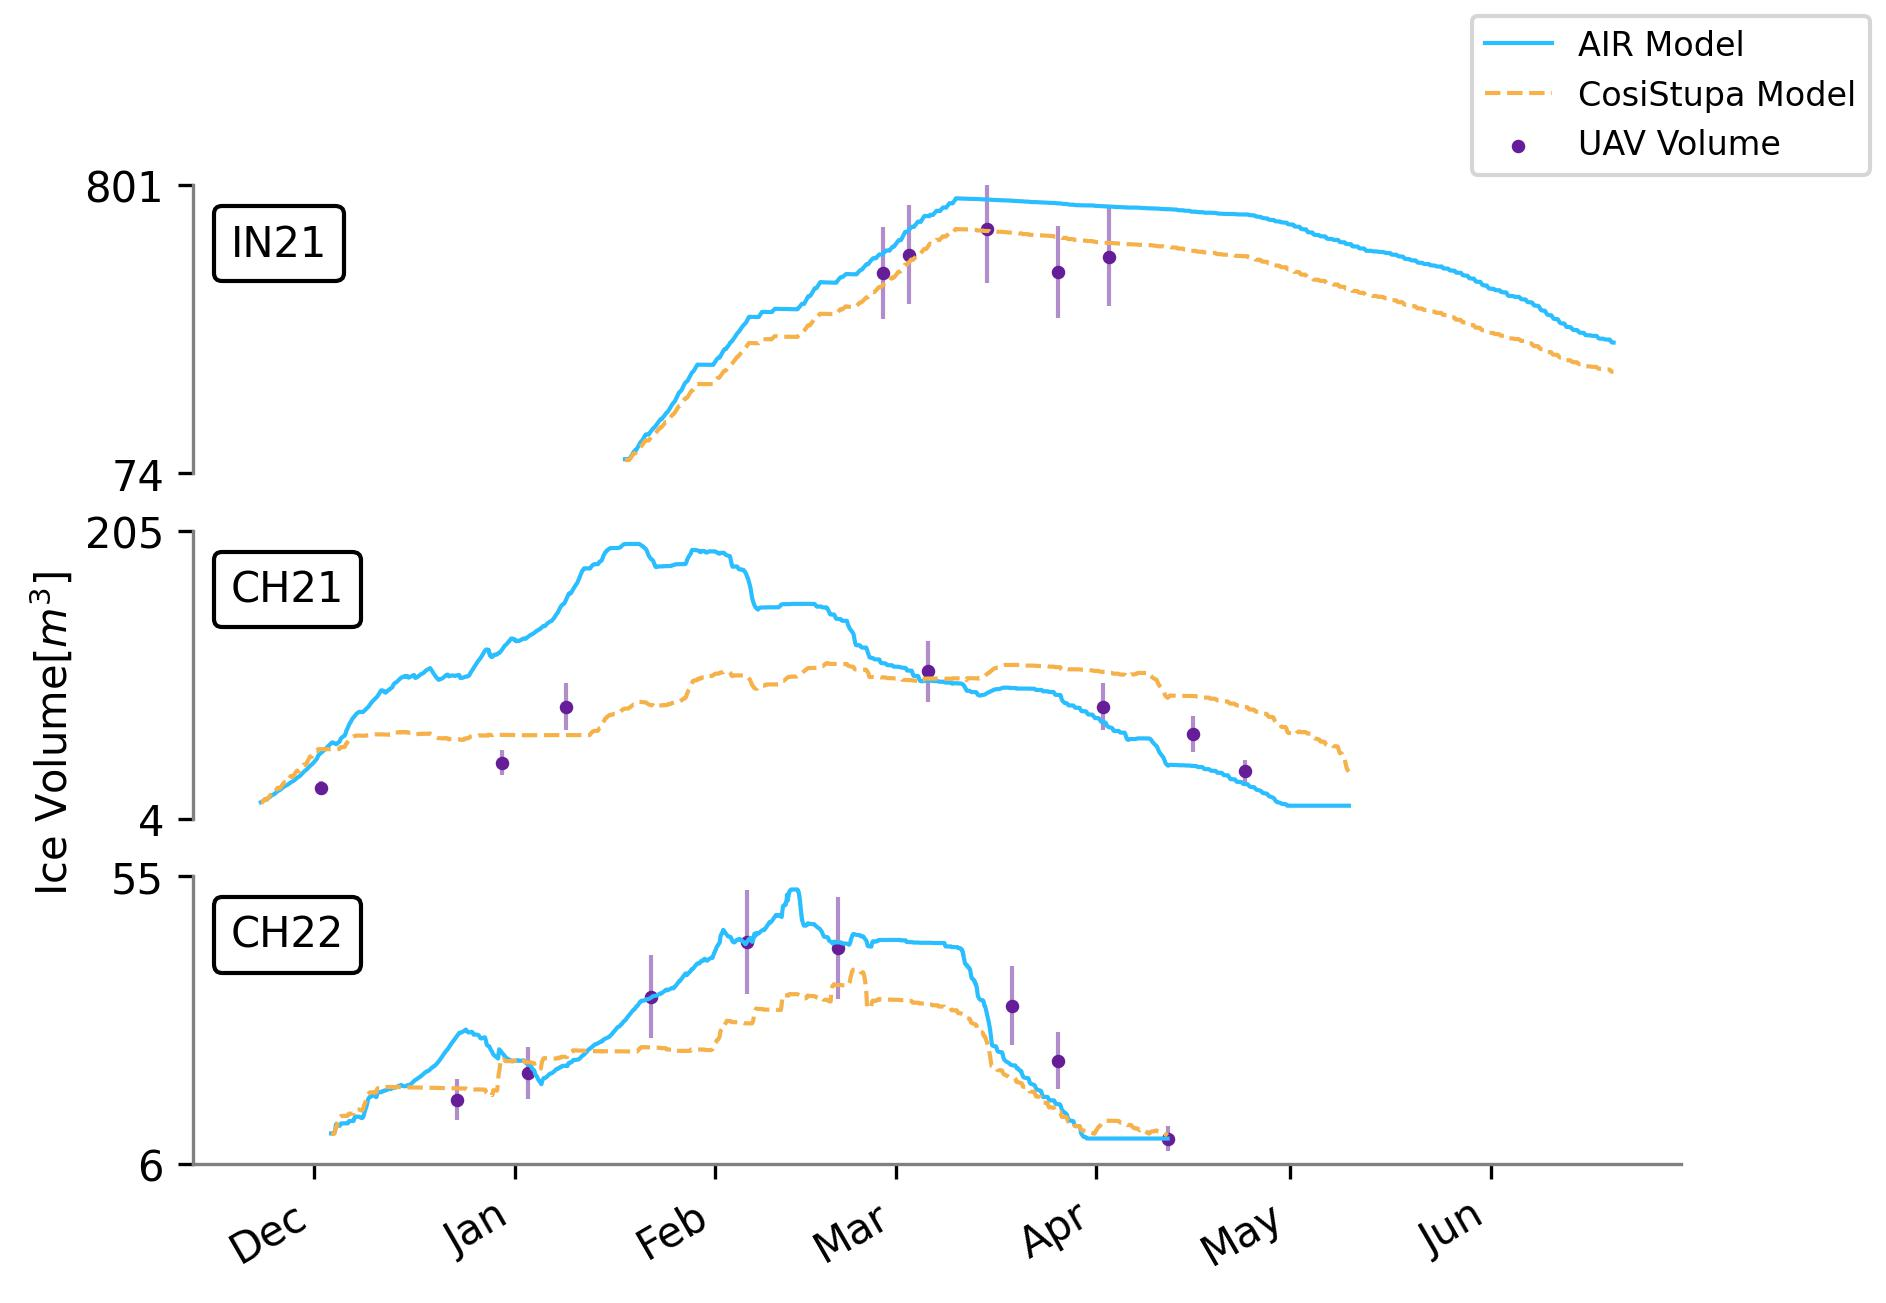
\includegraphics[width=12cm]{figs/model_compare.jpg}

\caption{}

\label{fig:Cosistupa}
\end{figure}

\section{Suggestions}

\subsection{Model limitations}

\subsection{Spray radius}

\subsection{Further data acquisition}

\subsubsection{Meltwater quantities}

The model validation set can be extended if daily AIR meltwater is measured. This dataset could serve as a
superior way to validate the model compared to the drone surveys which are also used for determining the spray
radius. However, the study site needs to satisfy two condintions in order to do this. First, the terrain of the
site needs to be waterproof and oriented so that most of the AIR runoff can be collected. Second, the chosen
location should not have high wind speeds, otherwise a significant fraction of AIR wastewater would be dispersed
in the air.

\subsubsection{Fountain characteristics}

Fountain pressure

\subsubsection{Drone flight analysis}

Identification of AIR boundary is subjective.

\subsection{Improvement of model algorithm}

\subsubsection{Initialisation of model}

\subsubsection{Better model parametrisations}

For turbulent fluxes

For other shapes/ shape evolution

Albedo variation due to fountain




   % INCLUDE: related work
\chapter{Technology of ice reservoirs}
\label{chap:tech}

\cleanchapterquote{In building ice stupas, it's necessary to engage enough workforce to extract the water over
	long distances and to keep water flowing in cold temperatures.}{Marcus Nüsser}{(Professor, South Asia Institute)}

Identifying which combination of interventions optimizes the return-on-investment and adaptive capacity in view
of future climate uncertainty remains a challenge, especially in arid mountain regions. It is expected that
mountains will experience stronger warming than lowlands \citep{ragettliContrastingClimateChange2016}, which
makes them particularly prone to having negative effects on water resources, including the loss of water
regulation capacity. The implementation of adequate adaptation strategies will need to respond to these changes,
as well as a growing anthropogenic demand for water \citep{buytaertWaterCitiesImpact2012}.

In this context, mountain communities have attempted many different ways of increasing artificial water storage
and improving hydrological regulation of their catchments \citep{ochoa-tocachiPotentialContributionsPreInca2019,
	ipccChapterHighMountain2019, ipccCrossChapterPaperMountains2022}. Developing ice harvesting structures is one of
these solutions that can play a role in increasing water security of mountain catchments.


\begin{figure}[htb]
	\centering
	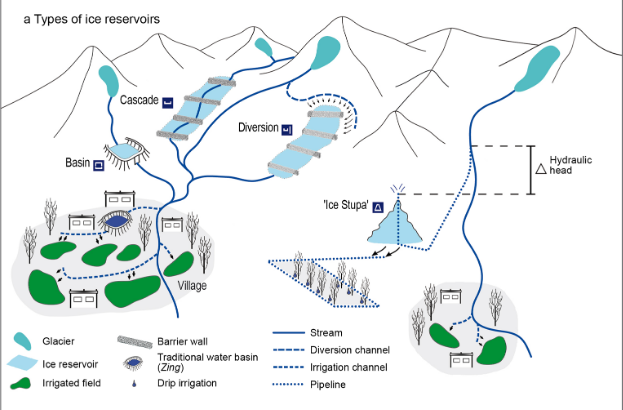
\includegraphics[width=\textwidth]{figs/AIR_designs}
	\caption{Different types of ice reservoirs. Adapted from \cite{nusserSociohydrologyArtificialGlaciers2019}.}
	\label{fig:AIRdesigns}
\end{figure}

In this chapter, we describe the different construction strategies of ice reservoirs ( Fig.
\ref{fig:AIRdesigns}). Later, we leverage our AIR models to propose engineering options and validate the
reduction in water losses and maintenance expected through them.


% \section{Traditional construction strategy}
\section{Types of ice reservoirs}

\subsection{Ice terraces}

According to oral history and satellite imagery from 1969, the first ice terraces are older than 50 years and can
be found in Phuktse and Igoo villages of Ladakh. Over the past 30 years, 14 ice terraces have been constructed in central Ladakh,
located in tributary valleys of the Indus \citep{norphelArtificialGlacierHigh2009,
	nusserSociohydrologyArtificialGlaciers2019}. Chewang Norphel, a well known engineer of the Leh Nutrition
Project, introduced this practice to Ladakh \citep{vinceGlacierMan2009}. Cascades and diversions shown in Fig.
\ref{fig:AIRdesigns} constitute the ice terrace type of AIRs.

\begin{figure}[htb]
	\centering
	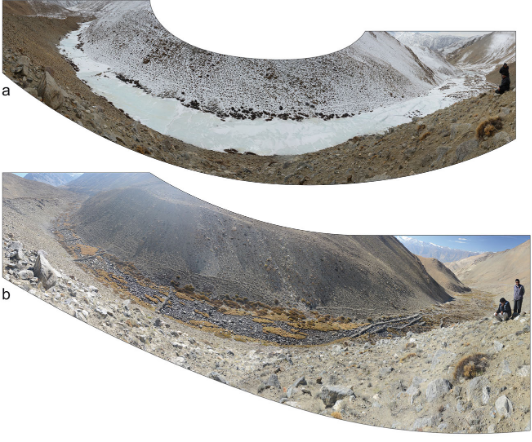
\includegraphics[width=\textwidth]{figs/IT_example.png}
	\caption{Ice terrace of Phuktse, viewpoint 4430 m. (a) February 2014 (b) October 2014 Adapted from:
		\cite{nusserSociohydrologyArtificialGlaciers2019}.}
	\label{fig:ITexample}
\end{figure}

There are two distinct types of ice terraces with site-specific modifications as shown in Fig.
\ref{fig:AIRdesigns}: the first type is built as cascades on perennial streams. A series of loose rock walls in
the river bed reduces flow velocity, but still lets water pass through. Such cascades allow flowing water to
freeze on exposed surfaces and form superimposed ice layers when temperatures drop ( Fig.
\ref{fig:ITscience}). An example of this is illustrated in Fig. \ref{fig:ITexample}.

The second type diverts water from streams with higher flow velocity to small side valleys, shaded by
surrounding mountains. This design allows to integrate higher slope positions for additional ice formation. It
consists of a series of partially cemented stone walls across the stream bed. Their dimensions are adjusted
based on the valley topography. The water for the ice terrace is obtained through a long diversion channel.

\begin{figure}[htb]
	\centering
	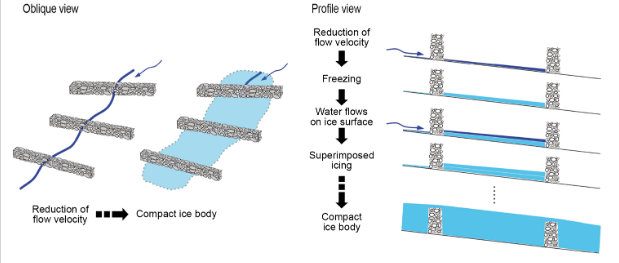
\includegraphics[width=\textwidth]{figs/IT_science.png}

	\caption{ The process of ice accumulation for ice terraces. Adapted from
		\citet{nusserSociohydrologyArtificialGlaciers2019}.}

	\label{fig:ITscience}
\end{figure}

The following construction guidelines are applied depending on the terrain of the construction site
\citep{norphelSnowWaterHarvesting2015}:

\begin{itemize}

	\item If the section of the stream is very wide with a mild slope, then stone walls are
	      constructed in a series parallel to each other. The number and dimension of ice-retaining walls depend on
	      the flow of water available in the main stream during peak winter.

	\item If the section of the stream is narrow with a steep gradient then it needs to be diverted to a shady area
	      by constructing a gravitational channel with sufficient slope. When it reaches the ice terrace site the
	      inclination should be gradually reduced, allowing the water to flow through small outlets thus accelerating freezing. Stone
	      walls need to be constructed parallel to the channel in series, according to the natural slope of the terrain.
	      The steeper the terrain, the smaller the distance and slope between the bunds.

\end{itemize}


\subsubsection{Water storage and cost}

The volume variations of ice terraces within Ladakh range from 510 $m^3$ to 81,040 $m^3$ highlighting
the importance of local topography and microclimate in their formation
\citep{nusserSociohydrologyArtificialGlaciers2019, norphelSnowWaterHarvesting2015}. The cost of construction
depends on the size and number of stone walls required. The estimated material cost of ice terraces vary between
4600 to 15,330 USD \citep{nusserSociohydrologyArtificialGlaciers2019}. The building of ice terraces also relies
on the participation of village communities for construction and maintenance.

\subsection{Ice stupas}

\begin{figure}[htb]
	\centering
	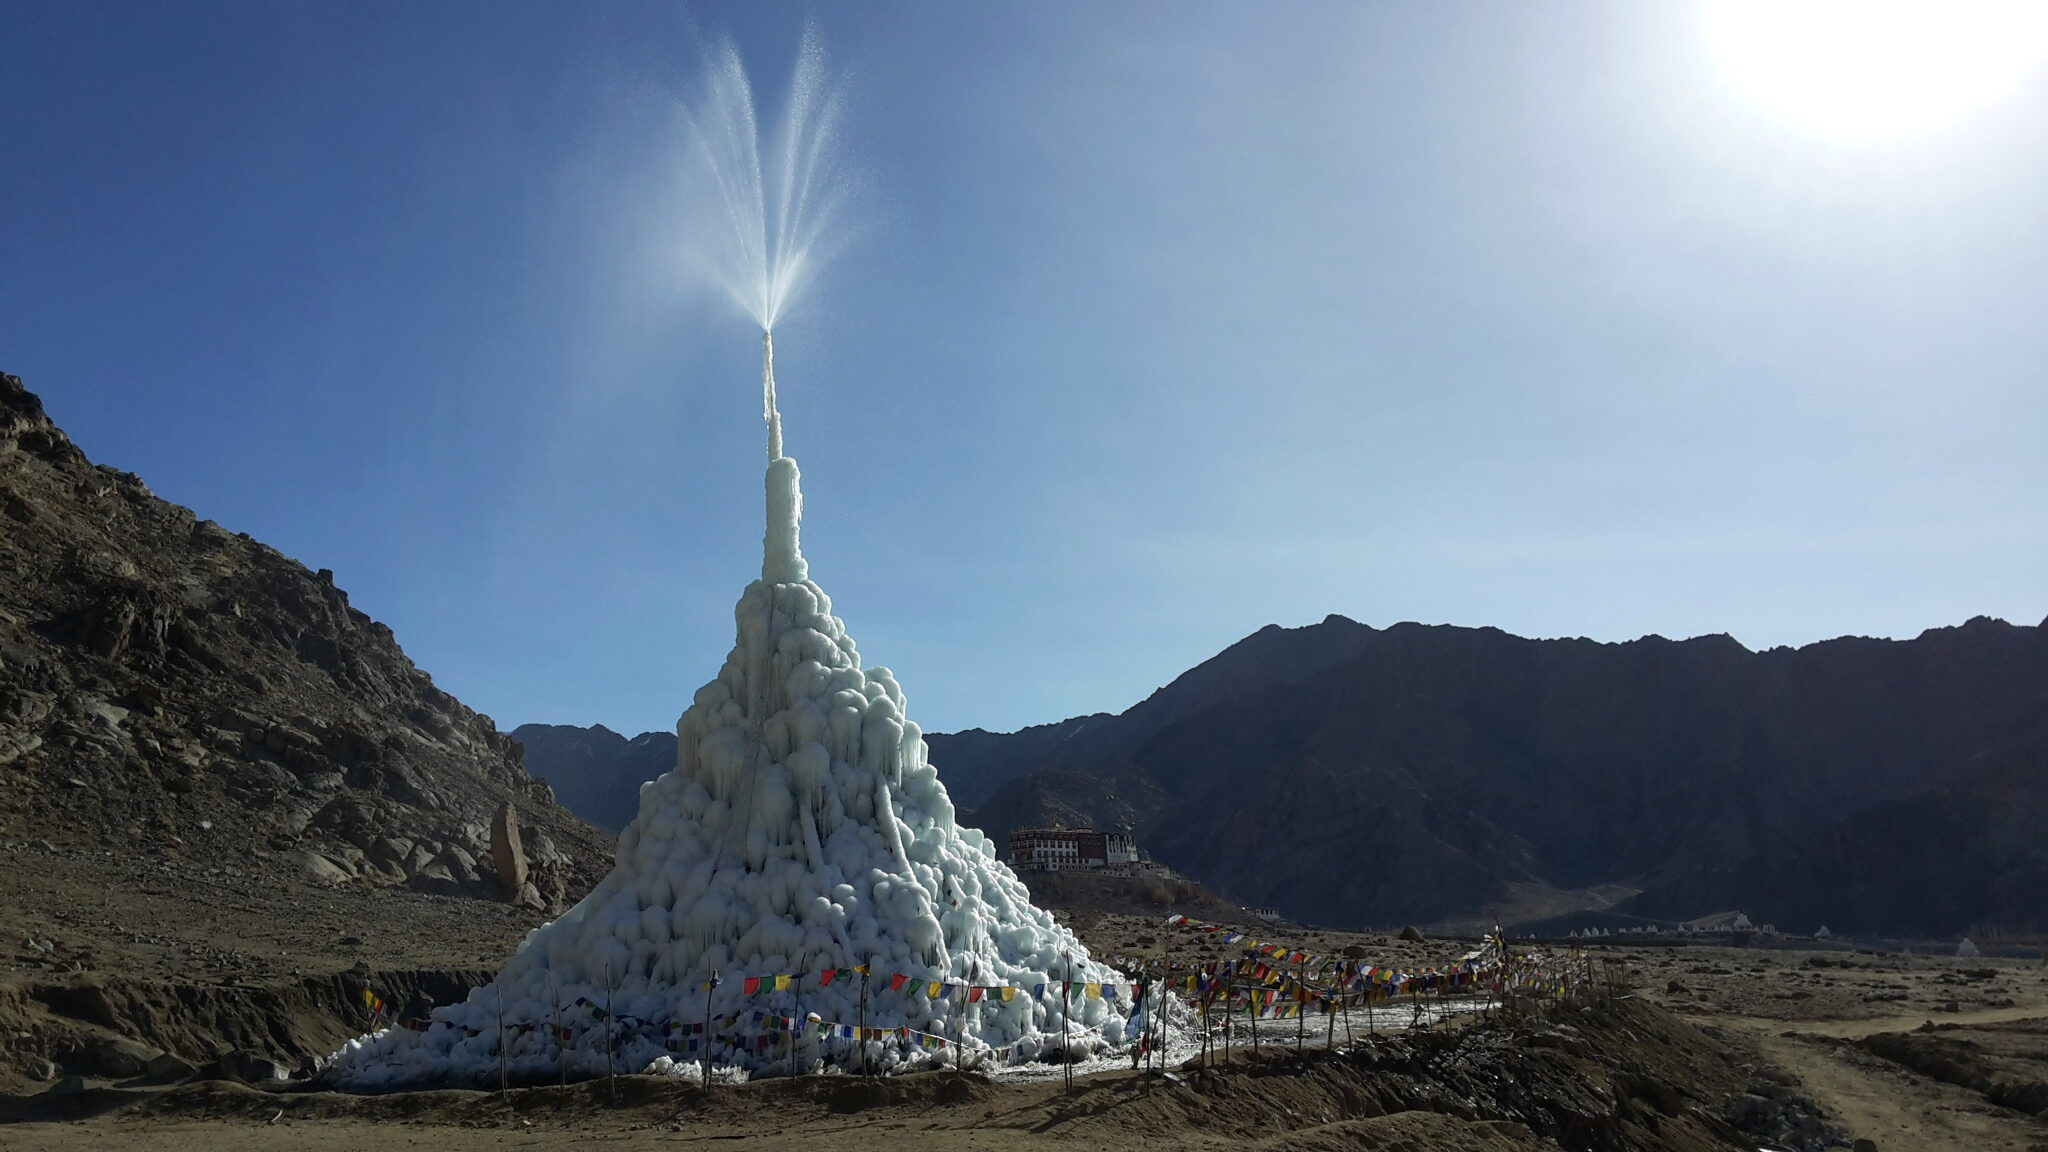
\includegraphics[width=\textwidth]{figs/IS_example.jpg}
	\caption{Ice stupa of Phyang village on March 2015. (P.C. Sonam Wangchuk)}
	\label{fig:ISexample}
\end{figure}

Ice stupas, invented by Sonam Wangchuk in 2013, provide a much easier way to achieve water storage compared to
ice terraces \citep{wangchukIceStupaArtificial2014}. Ice stupas can be placed much closer to the plantations
since they absorb less solar radiation per unit of volume compared to ice terraces due to their conical shape.
However, the typical volume range of ice stupas is also much smaller than that of ice
terraces \citep{nusserSociohydrologyArtificialGlaciers2019}. Over the past decade, several ice stupas have been
built to supplement irrigation water supply of mountain villages in India
\citep{wangchukIceStupaCompetition2020, palmerStoringFrozenWater2022, aggarwalAdaptationClimateChange2021},
Kyrgyzstan \citep{bbcnewsBrightArtificialGlacier2020}, Nepal and Chile
\citep{reutersConservationistsChileAim2021}.


\begin{figure}[htb]
	\centering
	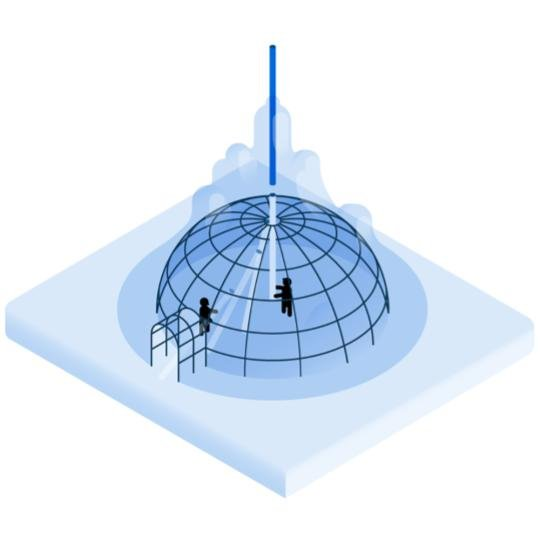
\includegraphics[width=8cm]{figs/IS_science.jpg}
	\caption{The construction process of ice stupas. Diagrams by: Francesco Muzzi }
	\label{fig:ISconstruction}
\end{figure}

A typical ice stupa simply requires a fountain nozzle mounted on a supply pipeline (Fig. \ref{fig:ISexample}).
The water source is usually a glacial stream. Due to the altitude difference between the pipeline input and
fountain output, water ejects from the fountain nozzle as droplets which freeze under subzero winter conditions.
The fountain is manually activated during winter nights. The fountain nozzle is raised through the addition of
metal pipes when significant ice accumulates below (Fig. \ref{fig:ISconstruction}). Typically, a dome of
branches is constructed around the metal pipes so that pipe extensions can be installed from within this dome.
Threads, tree branches and fishing nets are used to guide and accelerate the ice formation.

\subsubsection{Water storage and cost}

\begin{figure}[htb]
	\centering
	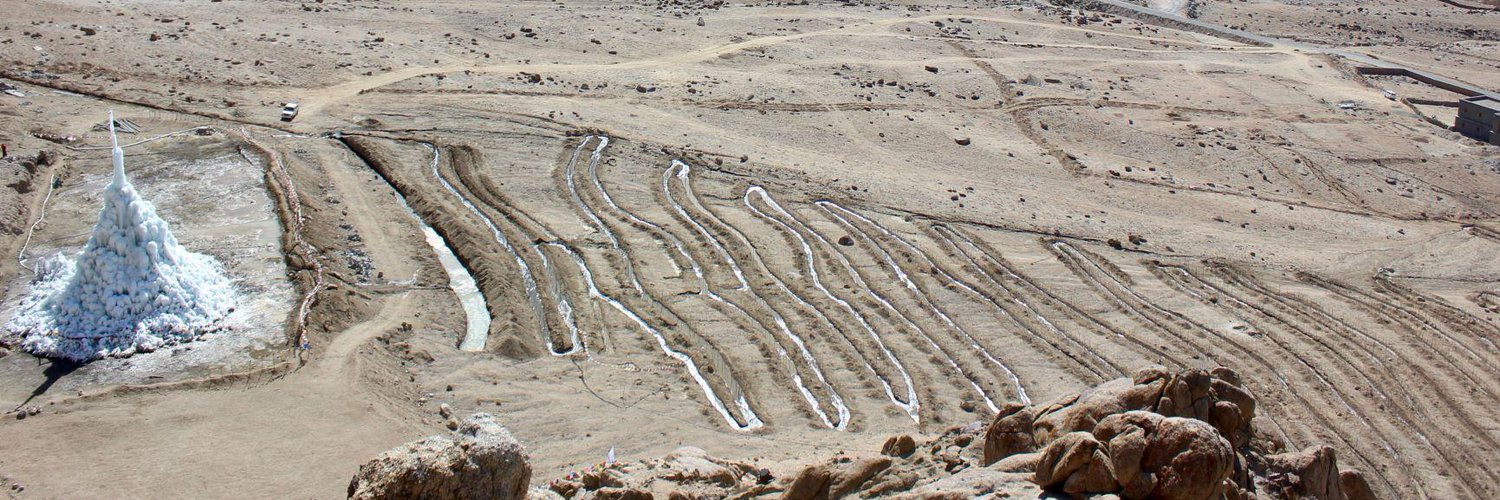
\includegraphics[width=\textwidth]{figs/IS_irrigation.jpeg}
	\caption{Irrigation channel of the ice stupa at Phyang village. (P.C. Lobzang Dadul) }
	\label{fig:ISirrigation}
\end{figure}

\begin{figure}[htb]
	\centering
	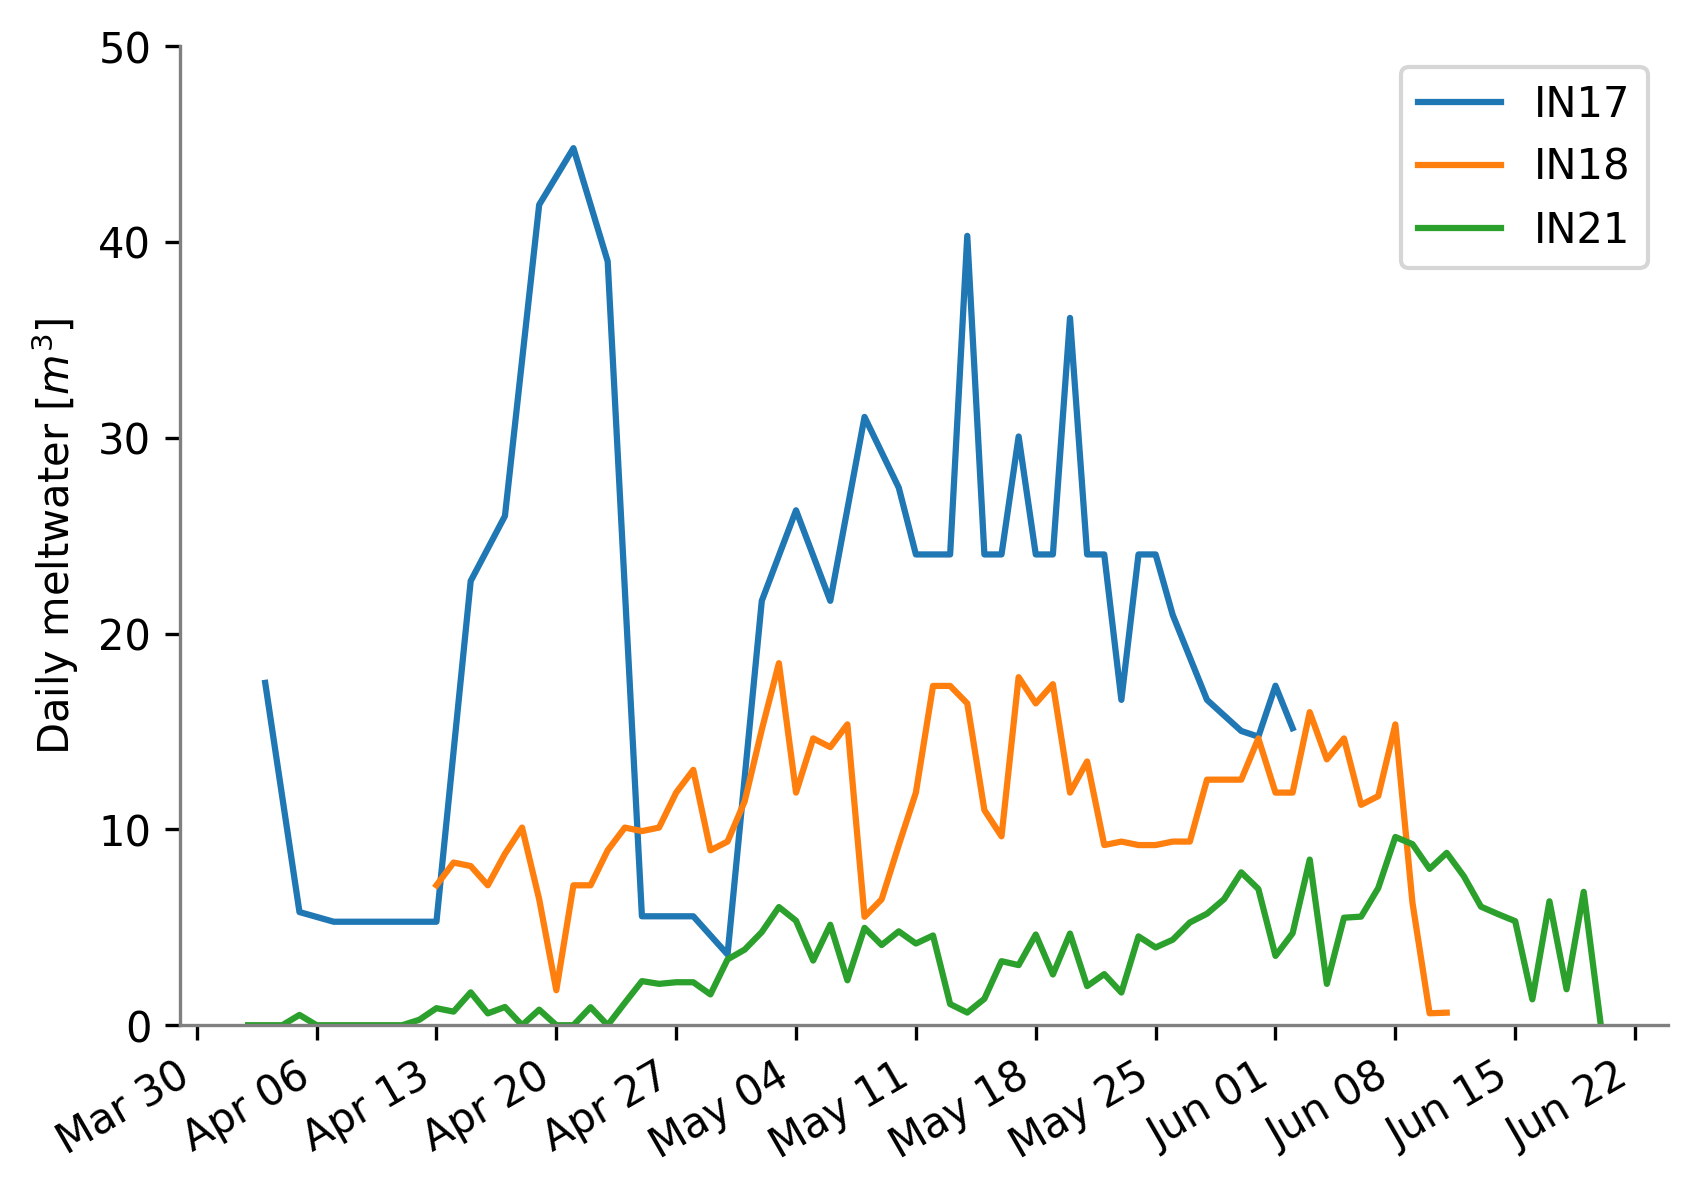
\includegraphics[width=\textwidth]{figs/melt.png}
	\caption{Daily meltwater measurements for the IN17 and IN18 AIRs along with the corresponding model estimations
		for the IN21 AIR. }
	\label{fig:ISmelt}
\end{figure}

The cost of construction primarily depends on the material, size and length of the pipeline required. The
fountain nozzle's cost is negligible in comparison. Typical pipeline configuration in Ladakh consists of a high
density polyethylene pipeline of 63 $mm$ diameter. The estimated cost of such a pipeline system is around 6,875
USD per $km$ of pipeline length.

Figure \ref{fig:ISmelt} shows the temporal variation of daily meltwater quantities obtained from 3 different
AIRs built in Ladakh during their melting periods (mid-April to mid-June). IN17 and IN18 AIRs were constructed
in Phyang village and their meltwater quantities were measured manually (Fig. \ref{fig:ISirrigation}). These
measurements were performed by recording the water level of a icestupa meltwater collection tank
\citep{vermaIceStupaMeltwater2018}. IN21 was constructed in Gangles village and its meltwater quantities
were modelled. The differences between the AIRs reflect the corresponding interannual variability in the weather
conditions. The median daily AIR meltwater quantities measured were higher than 11 thousand litres.

\section{The need for water supply management}

A common issue of AIR construction systems is water supply management, namely answering the questions "when to
water?", "how much?", and "for how long?". Starting water supply too early, spraying too much water, or
running water supply for too long might lead to overwatering; at the very least, this practice wastes water.
Similarly, starting the water supply too late, supplying too little water, or not running the water supply long
enough might lead to underwatering and can cause reduced ice volume. The management of water supply
differs based on the type of the AIR used. In the following analysis, we restrict ourselves to the ice stupa
form of AIRs where water supply management can also be referred to as fountain scheduling.

Paper I has shown that traditional ice stupa construction systems suffer from overwatering. For example, in
Indian AIRs, the fountain discharge rate could theoretically be halved since it is always twice as high as the
modelled freezing rate. However, in practice, the reduction of discharge rate could increase maintenance costs
due to higher risk of freezing events in the fountain pipeline.

An optimum construction strategy, therefore, should first prevent the occurrence of freezing events in the
fountain pipeline. These events can be prevented by setting a minimum threshold for the recommended discharge
rate. The discharge scheduler software developed in the previous chapter satisfies these requirements.

Adjusting the fountain discharge rate manually is not practical due to two reasons: first, this would involve
constant adjustments of discharge rates in response to the significant diurnal and seasonal variations of the
freezing rates; second, frequent pipeline water drainage would be required to avoid water losses. Therefore, operation
of scheduled fountains via automation systems is preferred to reduce long-term maintenance costs. The
hardware used to implement such an automation system is described in paper II.

This section aims to compare the water-use efficiency, maximum ice volume and maintenance effort between
traditional and automated construction strategies. First, two AIRs were built in the same location but with and
without automated fountain scheduling strategies; both were measured and compared (Fig. \ref{fig:autovsman}).
The associated datasets and the methods used to analyze them are described in paper II. In a second step,
differences in construction strategies between the Indian and Swiss AIRs studied in previous winters were quantified
using model simulations. Later we discuss how these construction strategies can help scale the ice volumes and
survival duration of AIRs.

\begin{figure}[htb]
	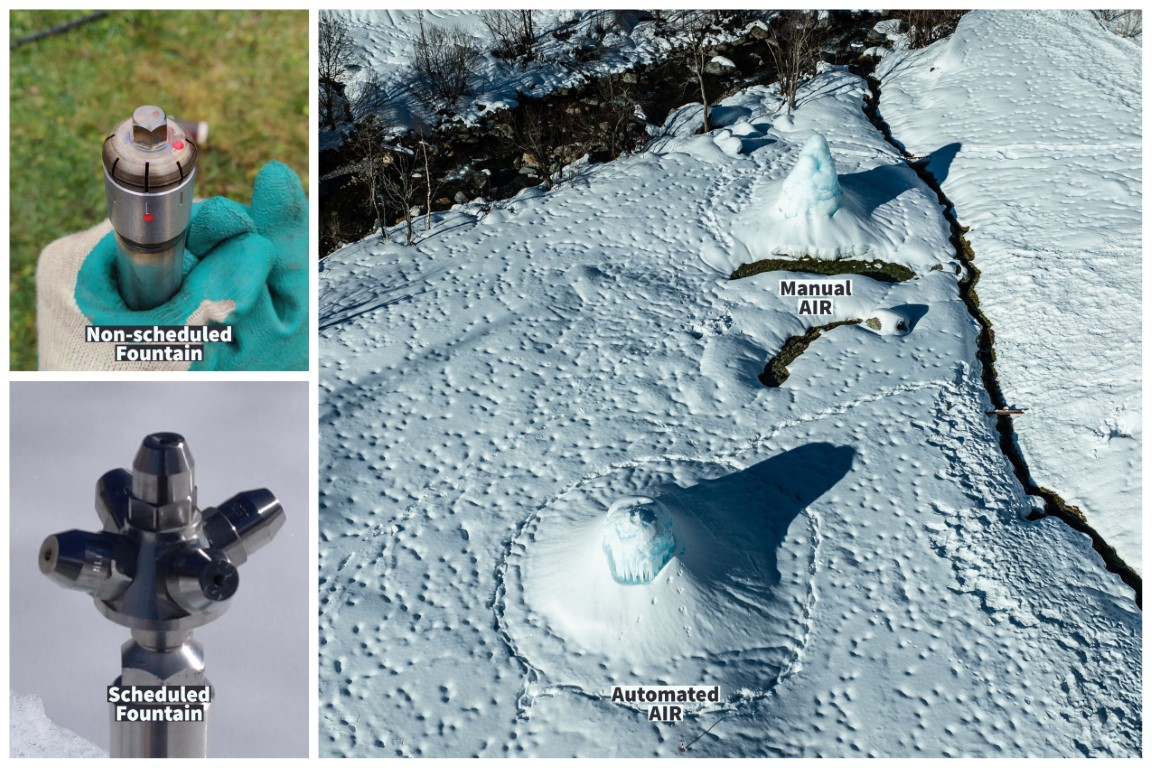
\includegraphics[width=\textwidth]{figs/AIR_fountains.jpg}
	\caption{Unscheduled and scheduled fountains used for construction of traditional and automated AIRs at Guttannen. Picture credits: Daniel Bürki}
	\label{fig:autovsman}
\end{figure}

\subsection{Automated fountain scheduling system}


Recommended discharge rates can only be produced if more information about the AIR surface properties and
weather conditions are available. Particularly, resolving the uncertainty in the expected freezing rate requires
quantification of the following three model variables: slope, albedo and cloudiness. But these properties cannot
be predicted beforehand. Therefore, we instead associate the upper and lower bound of each variable to a
different model depending on whether they increase the freezing rate or not. Higher slope and albedo values
decrease the shortwave radiation impact. Higher cloudiness values increase both the shortwave and the longwave
radiation impact. The model overestimating the freezing rate will be referred to as \ac{IVOM} and the model
underestimating the freezing rate will be referred to as  \ac{WEOM}, respectively. Accordingly, the values
assigned for all the three variables in the respective model is shown in Table \ref{tab:assumptions}.

The fountain scheduling software implements two types of fountain scheduling strategies depending on which
model type is suitable. WEOM model type is used if the location has limited water availability since it is expected to
produce better water-use efficiency. \ac{IVOM} model type is used if the location had limited duration of favourable
weather windows since it is expected to produce higher ice volumes. These two kinds of scheduled fountains will
be referred to as water-sensitive fountain and weather-sensitive fountain henceforth.

\begin{table}[htb]
	\centering
	\caption{Assumptions for the parametrisation introduced to simplify the ice volume optimised model (IVOM) and
		water-use efficiency optimised model (WEOM). $\alpha_{snow/ice}$ represents albedo of snow or ice respectively.}
	\label{tab:assumptions}
	\begin{tabular}{|lllll|}
		\toprule
		\textbf{Estimation of}          & \textbf{Symbol} & \textbf{IVOM}   & \textbf{WEOM}  &                       \\\midrule
		\multicolumn{1}{|l}{Slope}      & $s_{cone}$      & 1               & 0              & \multicolumn{1}{l|}{} \\
		\multicolumn{1}{|l}{Albedo}     & $\alpha$        & $\alpha_{snow}$ & $\alpha_{ice}$ & \multicolumn{1}{l|}{} \\
		\multicolumn{1}{|l}{Cloudiness} & $cld$           & $0$             & $1$            & \multicolumn{1}{l|}{} \\\bottomrule
	\end{tabular}
\end{table}

We apply the assumptions described in Table \ref{tab:assumptions} on the one-dimensional description of energy
fluxes through Eqn. \ref{eqn:EB}. The derivation of the individual energy and mass balance terms for the
\ac{IVOM} and \ac{WEOM} model versions are discussed in the Appendix \ref{sec:auto_software}.

Equation \ref{eqn:EB} is implemented in the automation software. The user interface of the software enables
input of the spray radius, altitude, latitude and longitude of the construction location. The automation
hardware consists of an AWS, flowmeter, control valve, drain valves, air valves, fountain, pipeline and a
logger. The logger feeds the AWS data to the automation software and informs the recommended discharge rate to
the flowmeter. The flowmeter adjusts the control valve to match the recommendation. When a termination
criteria is met, the drain and air valves allow the removal of water from the pipeline and the entry of
air in the pipeline respectively.

The recommended discharge rate is equal to the mass change rate. However, certain termination criteria listed
below override the discharge rate recommendation and drain the pipeline to prevent water loss or fountain
freezing events:

\begin{itemize}

	\item High water loss is assumed if wind speed is greater than the user-defined critical wind speed.

	\item High risk of fountain freezing event is assumed if mass change rate is lower than the user-defined minimum fountain discharge rate.

	\item Freezing events in the fountain pipeline are assumed if measured discharge rate is zero for at least 20
	      seconds.

	\item Pipeline leakage is assumed if measured discharge rate is greater than the user-defined maximum fountain discharge rate.

\end{itemize}

\subsection{Comparison of traditional and automated construction strategies}

\begin{figure*}[htb] 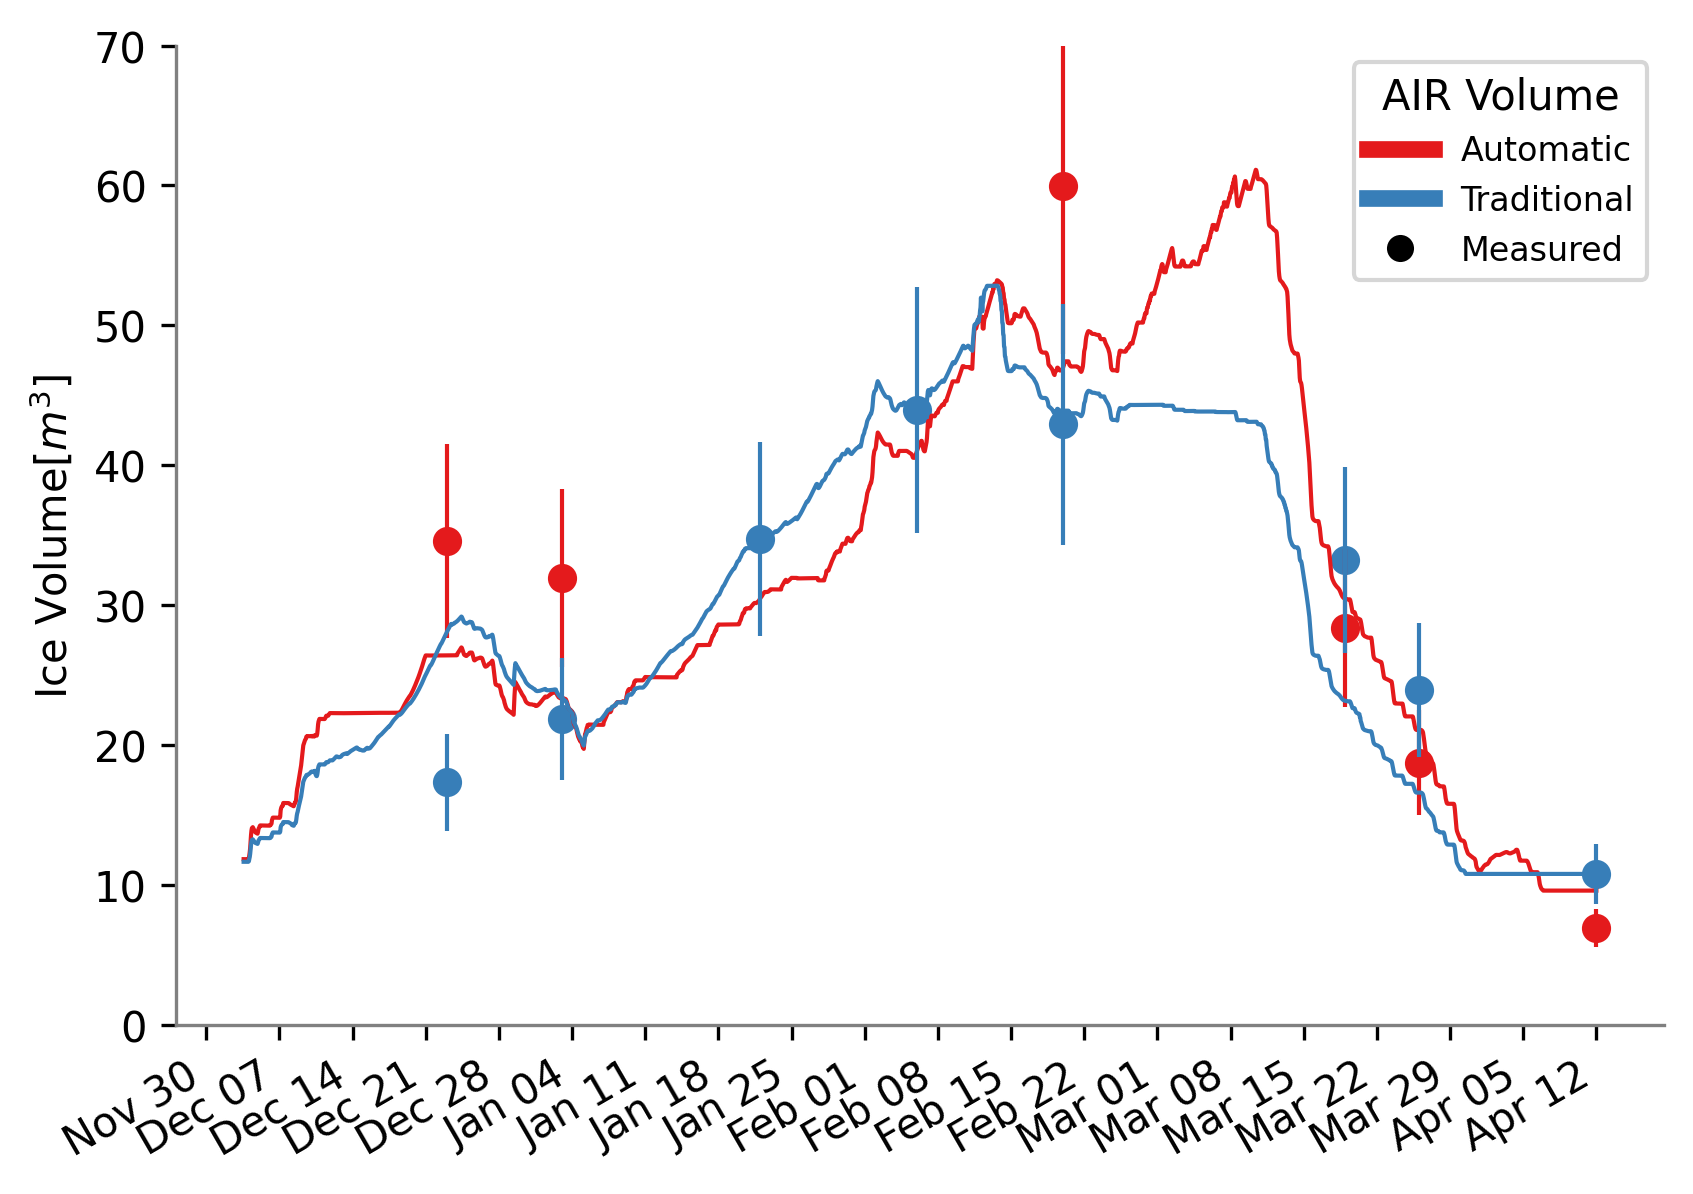
\includegraphics[width=\textwidth] {figs/CH_validation.png} \caption{Volume validation of the
		scheduled and unscheduled fountain construction strategies.} \label{fig:validation} \end{figure*}

Fountain scheduling reduced the fountain discharge input and fountain wastewater output by an order of
magnitude. However, this does not result in an appreciable difference in the volume evolution of the automated
or traditional AIR, as shown in Fig. \ref{fig:validation}. This is due to two counteracting surface processes
during fountain spray: process A consists in the dampening of albedo to ice albedo and process B consists in the
absorption of heat energy from the fountain water droplets. The temporal variation of the magnitude of these
processes is shown in Fig. \ref{fig:dis_processes}.

\begin{figure*}[htb]
	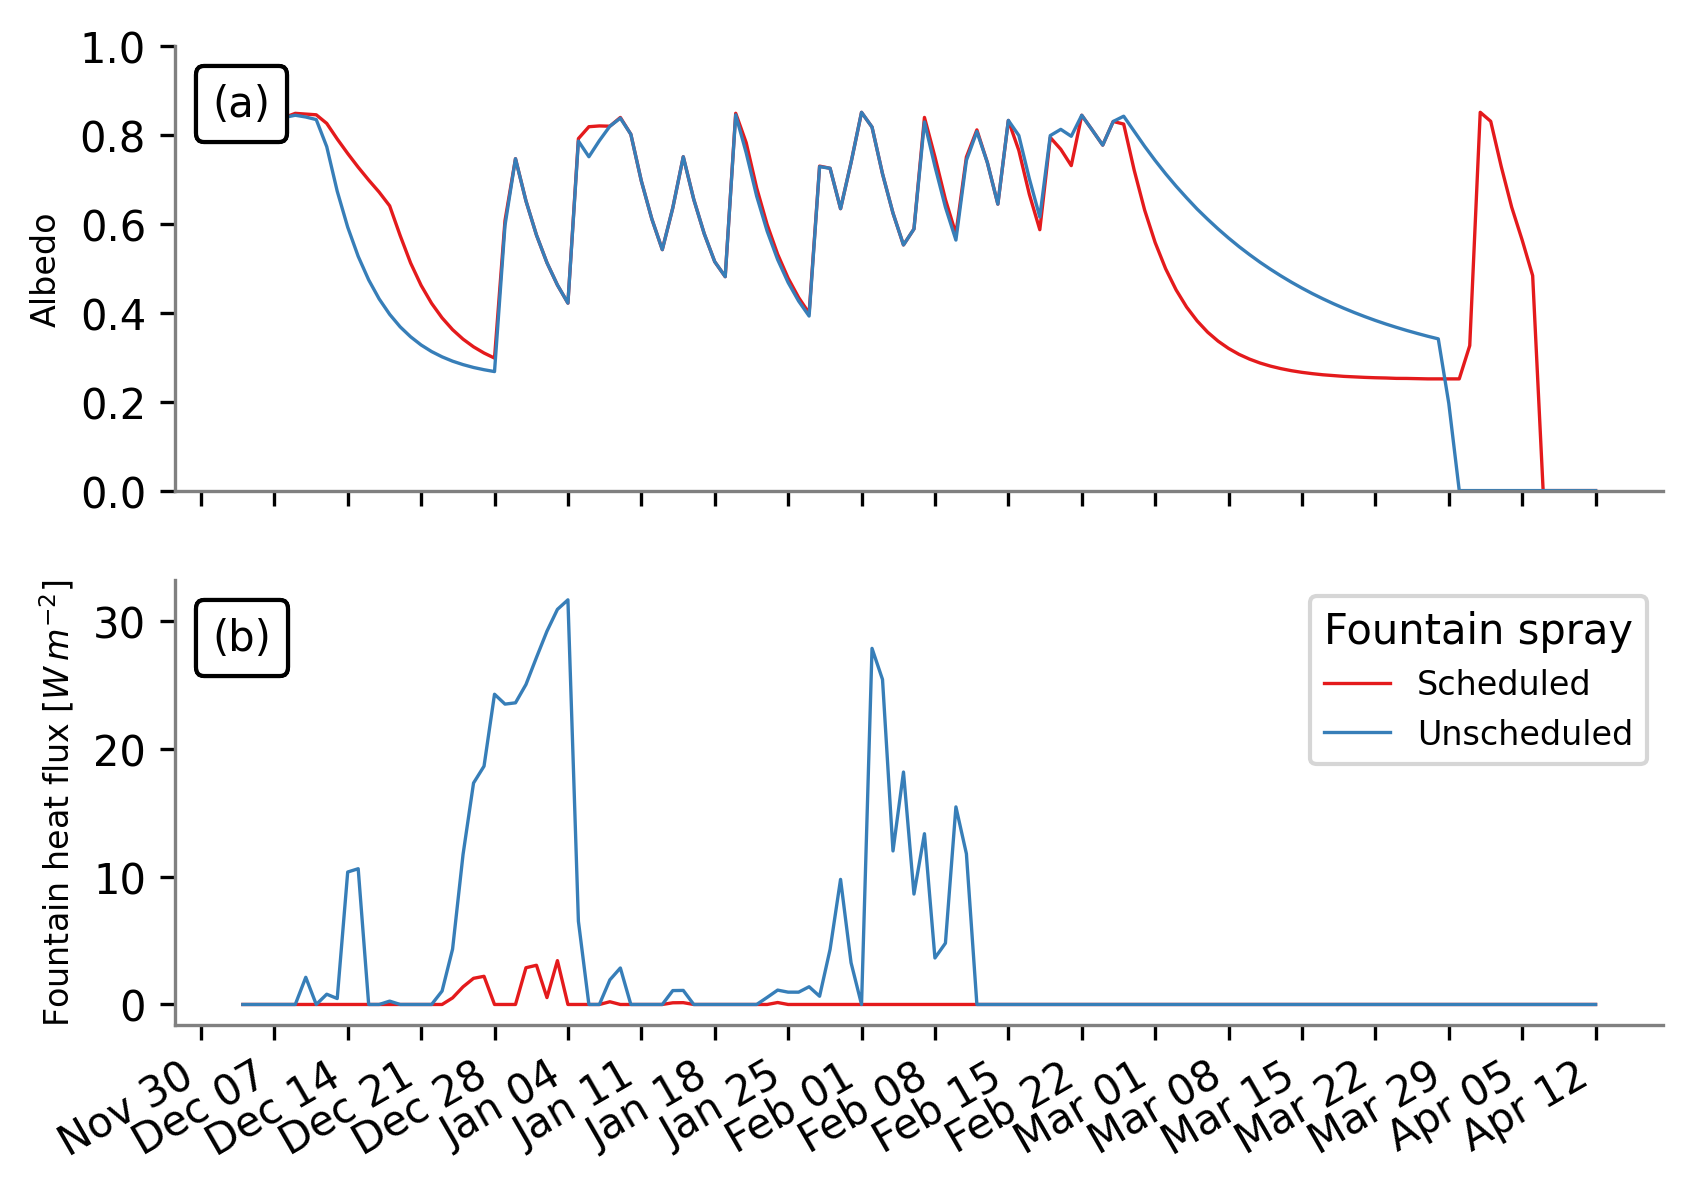
\includegraphics[width=\textwidth]{figs/dis_processes.png}
	\caption{(a) Surface albedo  and (b) fountain discharge heat flux showed significant variations between the two
		AIRS due to the differences in their discharge rates.}
	\label{fig:dis_processes}
\end{figure*}

The difference in water-use efficiency and maximum ice volume between unscheduled and scheduled fountains in the
Indian and Swiss locations across two winters is shown in Fig. \ref{fig:wue}a. Four experimental values
(highlighted in circles) and five simulated values (highlighted in squares) are shown together.  The
experimental values were taken from the IN21 and CH21 AIRs studied in paper I and the CH22 AIR investigated in
paper II.

\begin{figure}[htb]
	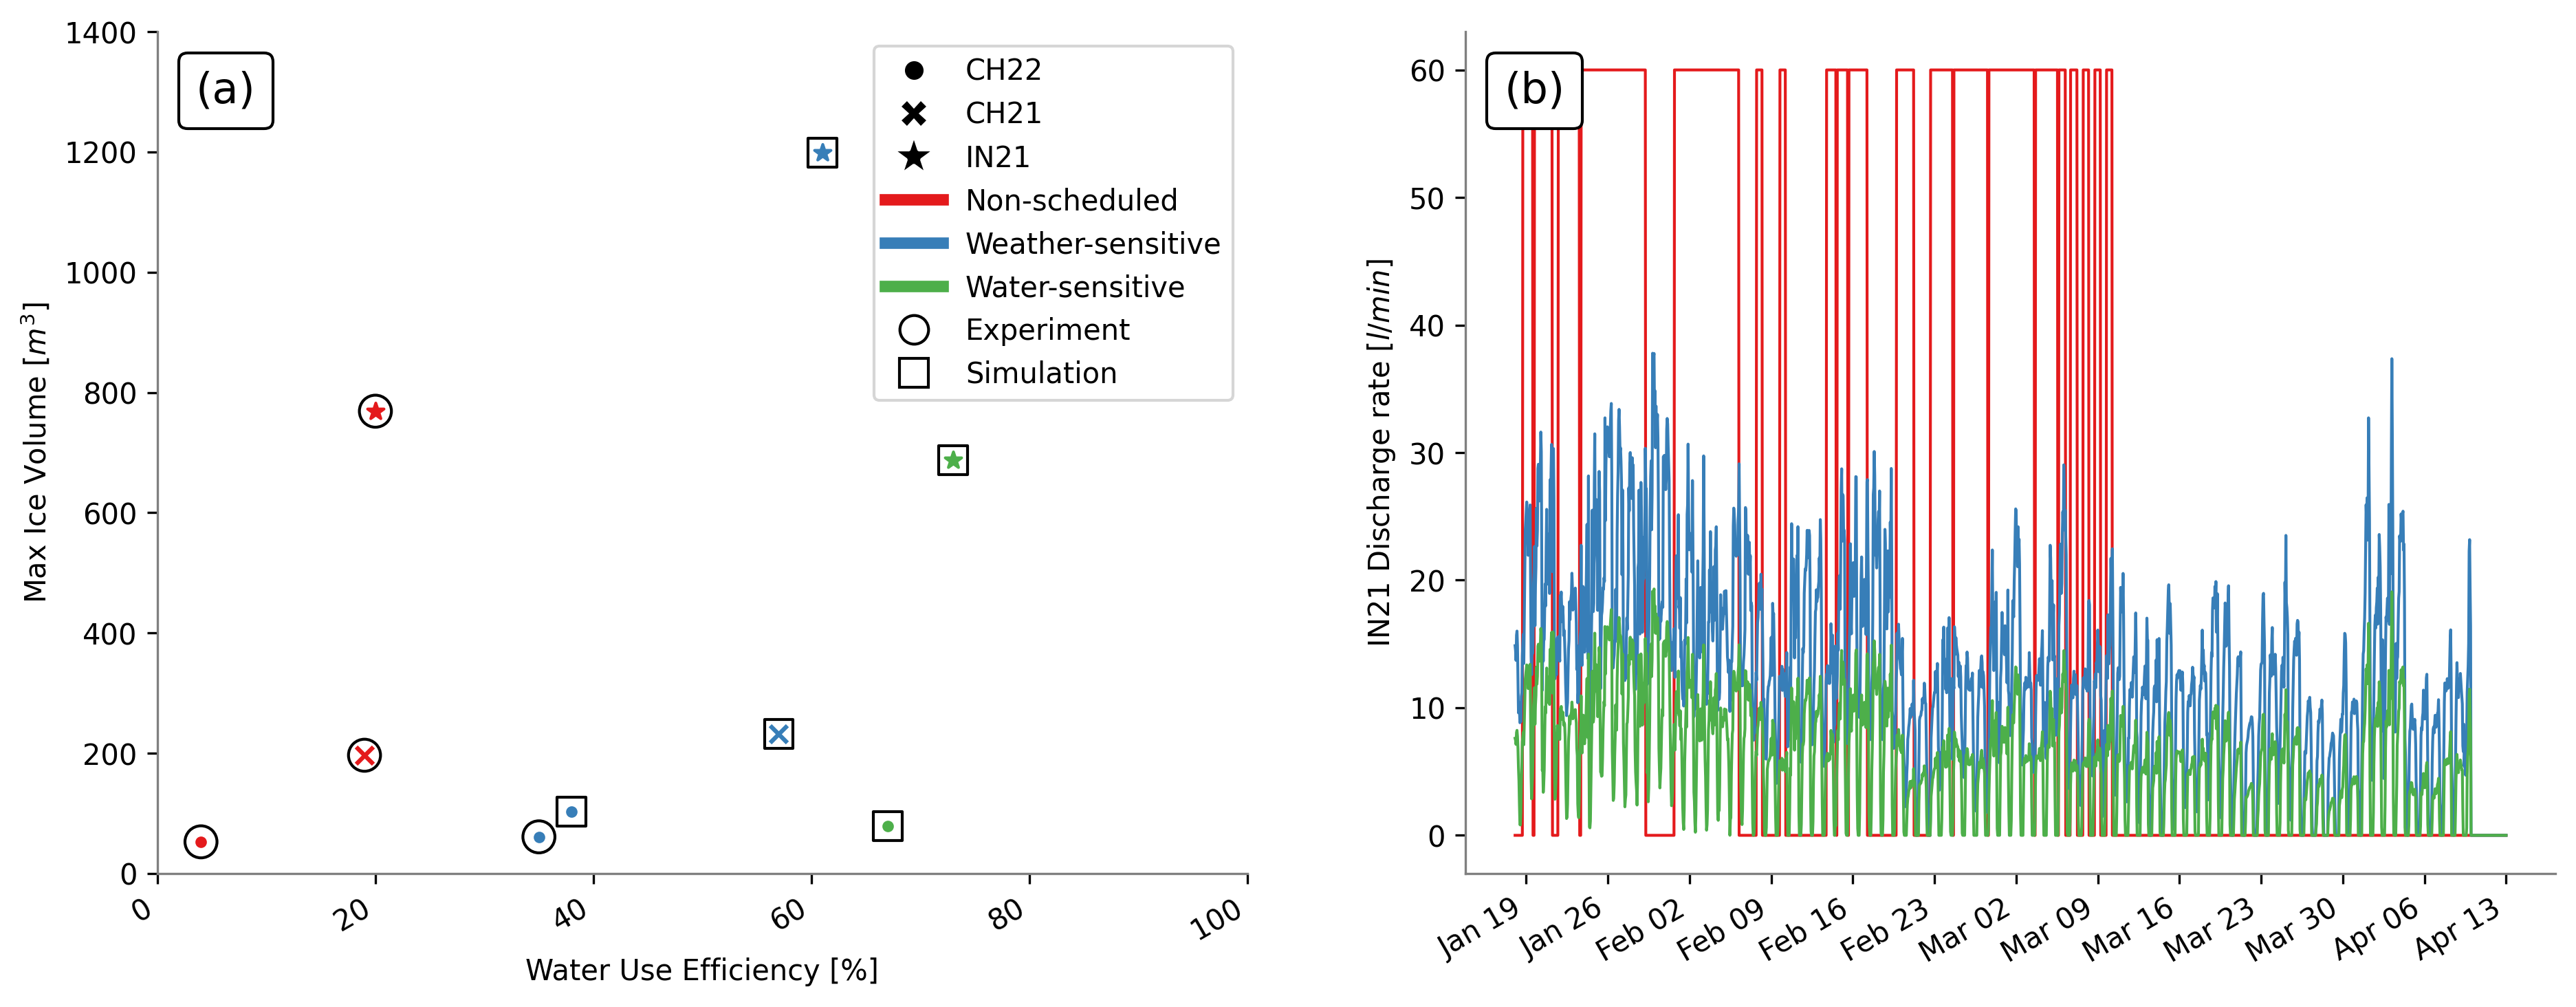
\includegraphics[width=\textwidth]{figs/wue.png}

	\caption{(a) The maximum volume and water-use efficiency estimated for AIRs constructed in different locations
		(represented by symbols) with different fountain scheduling strategies (represented by colours). Experimental
		values are highlighted in circles and simulated values are highlighted in squares. (b) Comparison of
		the unscheduled and scheduled fountain discharge rates at the IN21 location.}

	\label{fig:wue}
\end{figure}

The water-use efficiency of all the unscheduled fountains is below 20 \%. In general, water-use efficiency
exhibits a threefold increase when the weather- or water-sensitive fountains are used in both
locations.

For the Indian location, the three different kinds of fountains yielded significantly different results owing to discharge
duration and max discharge rate
(Fig. \ref{fig:wue}b). The unscheduled fountain showed a maximum discharge rate more than twice that of
the scheduled fountains, resulting in higher water loss; freezing events in its pipeline caused frequent
interruptions in the unscheduled discharge rate (Fig. \ref{fig:wue}b). In contrast, the mean freezing
rates of the other two fountains during these events were above their median values. This is because very cold
temperatures freeze the water inside rather than outside the fountain system, instigating such freezing events in
the fountain pipeline. Therefore, the discharge duration of the unscheduled fountain was much lower, resulting in
lower ice volume. The water-sensitive fountain underestimated the freezing rate during the construction period
and therefore produced much lower ice volume compared with the weather-sensitive fountain.

For the Swiss locations, scheduled fountains yielded better water-use efficiency but did not significantly alter the maximum
volume obtained.

% AIRs, located at much lower
% altitudes than naturally occuring glaciers, serve to bridge the critical gap in water availability by providing
% meltwater earlier in the agricultural season. Such ice reservoirs utilize the hydrological process of icing
% under local conditions of frequent freeze-thaw cycles to capture water for seasonal storage. They are not water
% storage structures that freeze from the top down, rather they are produced through sequential, freezing of thin
% layers of water creating superimposed sheets of ice.
   % INCLUDE: related work
\chapter{Habitat of ice reservoirs}

\cleanchapterquote{Ice stupas offer a solution to the shortage of water all our mountain regions are
	facing.}{Pema Gyamtsho }{(Director General, International Center for Integrated Mountain Development)}

\ac{AIRs} cannot be built anywhere. They require favorable meteorological conditions, sufficient water supply,
and specific topography to amass a seasonal stock of ice. However, these three requirements are coupled and
exhibit drastic spatiotemporal variations. Therefore, generalizing results from \ac{AIRs} studied in this thesis to
obtain future volume estimates in new construction locations is plagued with uncertainty.

In this chapter, ice volume observations are leveraged to disentagle the relationship between meteorology
and topography to provide first-order estimates of interregional, intraregional, and interannual ice volume
variations. 

\section{Interregional ice volume variability}

\ac{AIRs} built in the Alps and the Himalayas show drastic ice volume variations. Comparison of ice stupa volume
evolution shows that the Indian structures grew four times larger than the Swiss ones (Fig. \ref{fig:2AIRs}). The
ice volume achieved after the accumulation period was much higher for the Indian ice stupa compared with the Swiss
ice stupas. The lower net radiation fluxes of the Indian location favored a faster thickness growth, and the
spray radius of the Indian fountain produced a larger surface area compared with its Swiss counterparts (paper I).
These results indicate that the colder, drier, and less cloudy meteorological characteristics of the Ladakh
region (Table \ref{tab:Observations}) make it more suitable to build \ac{AIRs} compared with the Guttannen region. 

\section{Intraregional ice volume variability}

\begin{figure}
	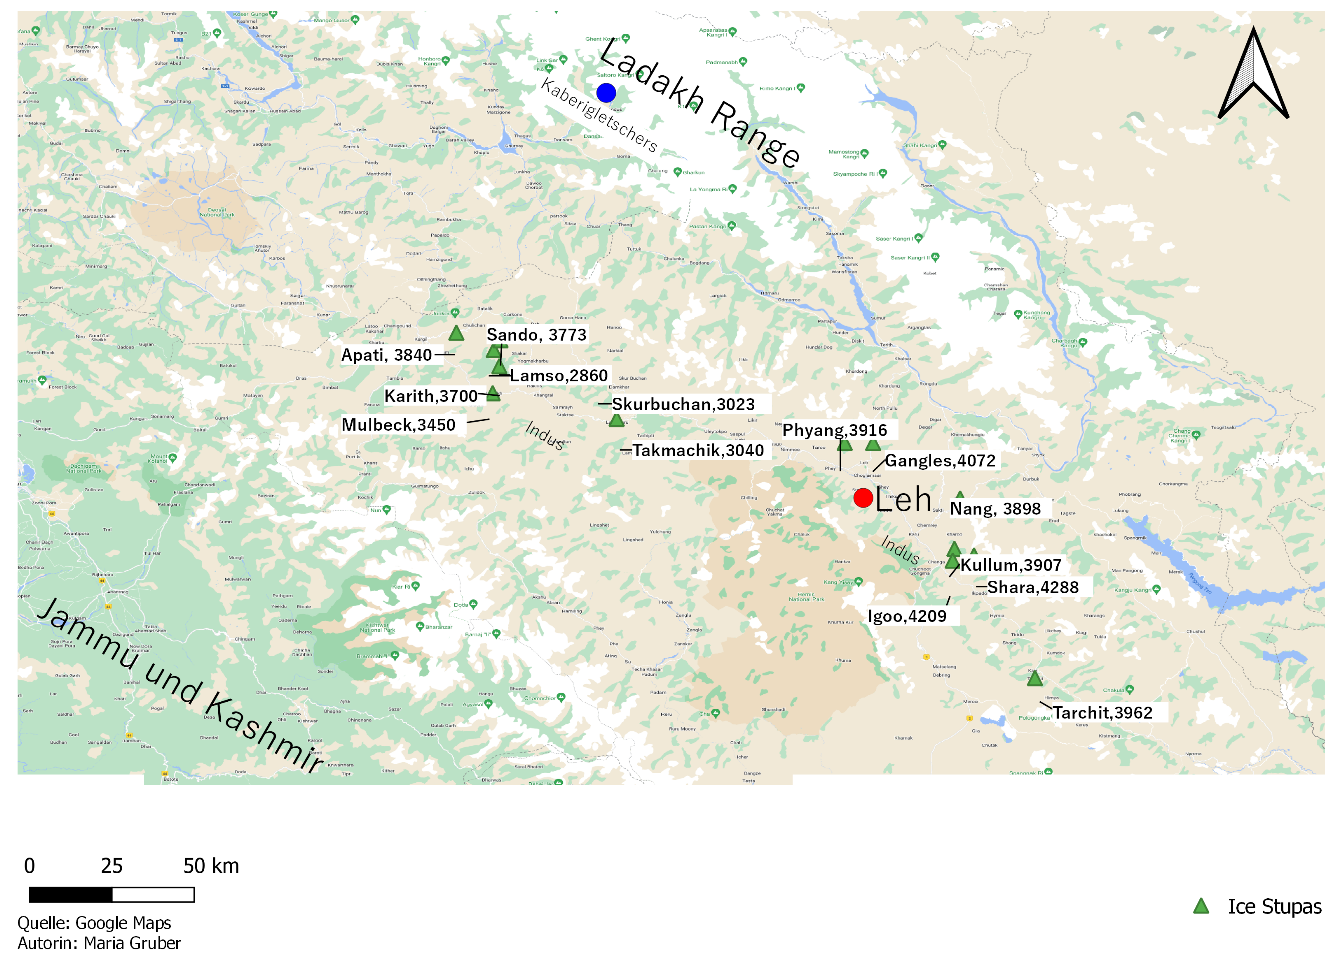
\includegraphics[width=\textwidth]{figs/ISC_villages}
	\caption{Villages of Ladakh for which ice stupa volume observations are available. Adapted from \citet{mariagruberIceStupasLadakh2022}.}
	\label{fig:villages}
\end{figure}

Ice volumes were measured in more than 14 villages in Ladakh (Fig. \ref{fig:villages}). Their volume variation
reveals a correlation with the altitude of the construction location (Fig. \ref{fig:altvsvol}). This correlation
indicates that an elevation gain of 100 $m$ causes a corresponding ice volume gain of 1 million $l$. However,
some locations at lower altitudes exhibit higher volumes compared with those at higher altitudes. This is due
to topographic effects of shadow valleys that reduce the sunshine hours of the location
\citep{mariagruberIceStupasLadakh2022}.

\begin{figure}
	\centering
	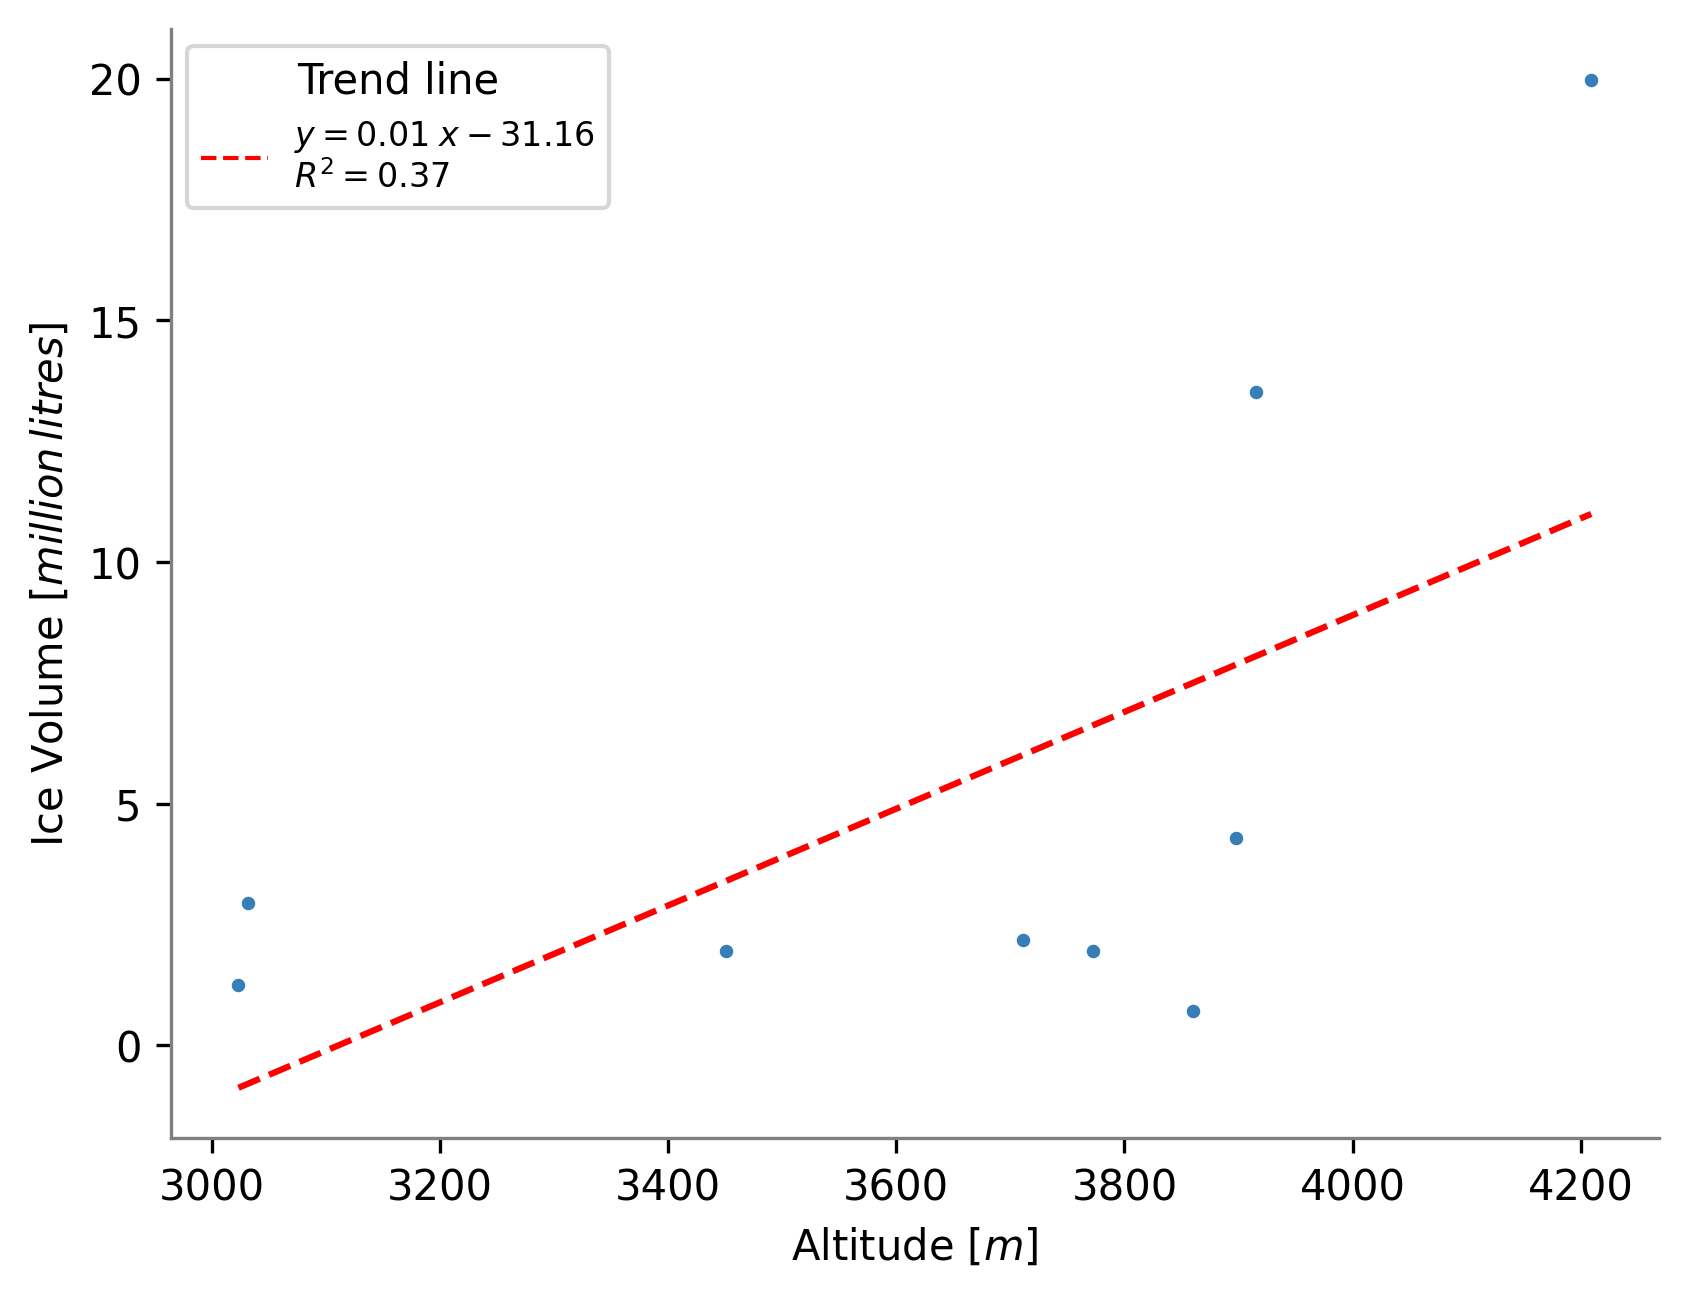
\includegraphics[width=\textwidth]{figs/altitudevsvolume.png}
	\caption{Relationship of measured ice volume (blue dots) with altitude of \ac{AIRs} built during the winter of 2019/20 across
		different villages in Ladakh. Adapted from \citet{mariagruberIceStupasLadakh2022}.}
	\label{fig:altvsvol}
\end{figure}

Two ice stupas built in villages above 4200 $m$ \ac{a.s.l.} (Shara and Igoo) have also been observed to last
beyond a summer melt season (Fig. \ref{fig:PIR}). However, such favorable meteorological conditions remain to
be discovered in the Swiss mountains. This question can be investigated by decreasing the air temperature to which
Swiss ice stupas are exposed to uniformly (temperature change $\Delta T$). This would imply a stronger negative
sensible heat flux in summer, thus accelerating ice stupa growth and slowing its decay. Such simulations
were produced using the Oerlemans model for an ice stupa grown in the Diavolezza site at an altitude of 2080 $m$
\ac{a.s.l.}. A break-even point for $\Delta T = -2 \degree C$ (Fig. \ref{fig:PIR_evolution}) was found. For
larger negative values of $\Delta T$, the ice stupa does not disappear in summer but keeps growing from year to
year. For $\Delta T = -3 \degree C$, the maximum volume in the fifth year is about four times that in the first
year (Fig. \ref{fig:PIR_evolution}). Therefore, we hypothesize that ice stupas can last beyond a year even in
Switzerland if built in locations with an elevation above 2388 $m$ (based on a standard atmospheric lapse rate
of 0.0065 $\degree\,C\,m^{-1}$).

\begin{figure}
	\centering
	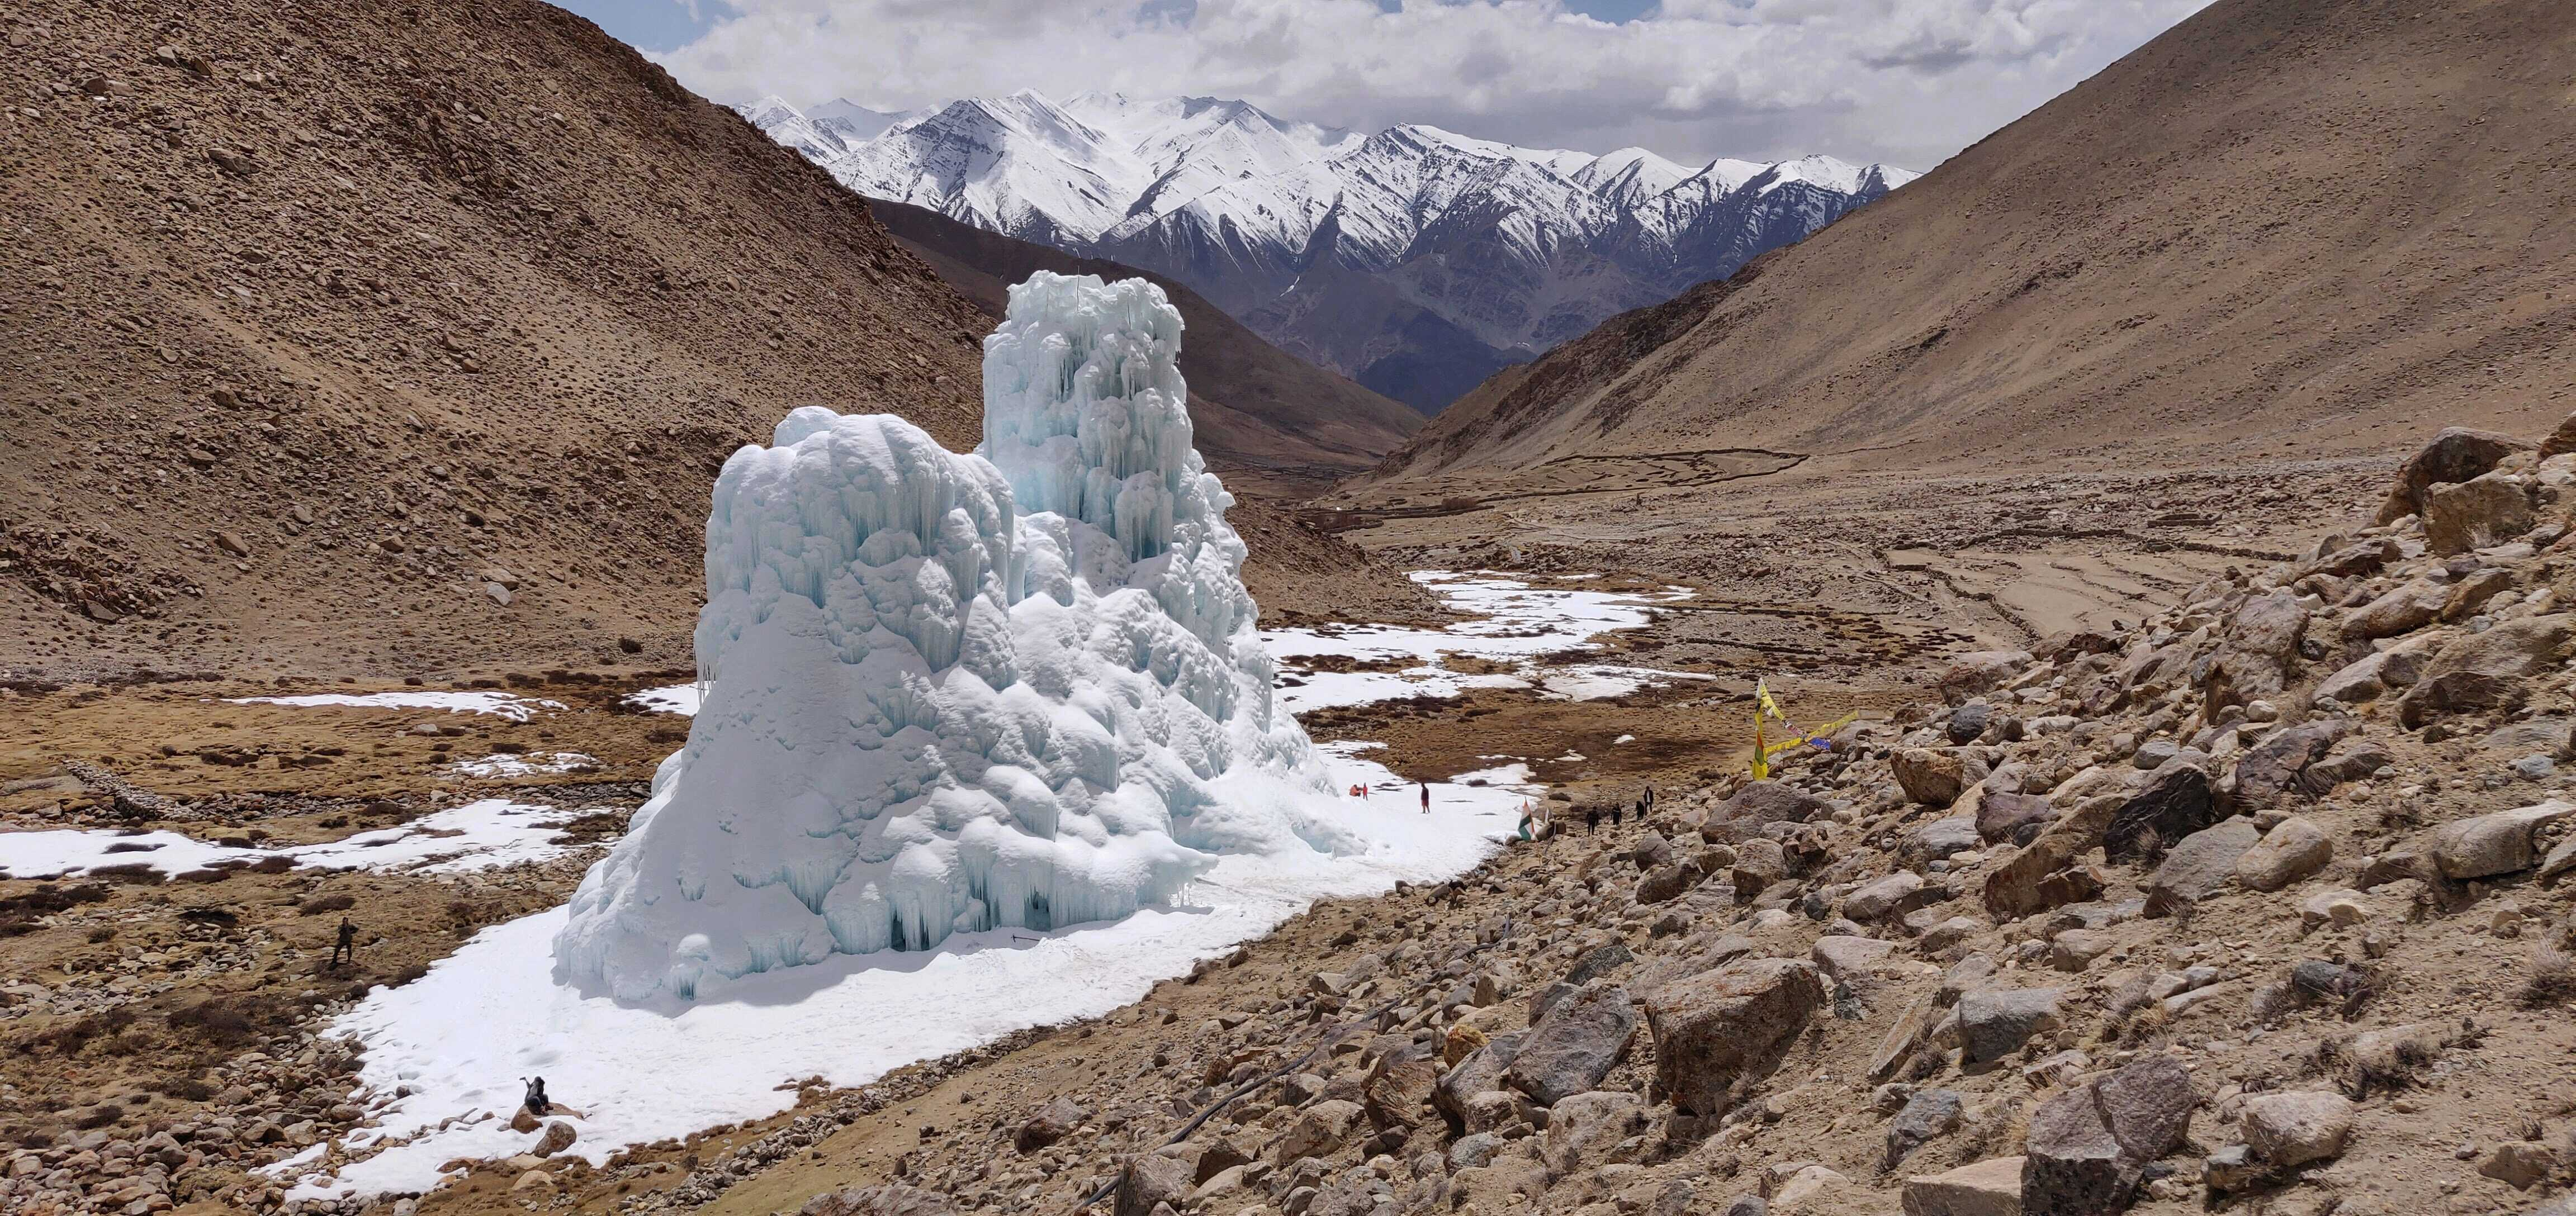
\includegraphics[width=\textwidth]{figs/PIR_example.jpg}

	\caption{Ice stupa at Shara, Ladakh, built by local farmers in the winter of 2019/20, survived a full summer melt season and released
		around 8 million $l$ of water.}

	\label{fig:PIR}
\end{figure}

\begin{figure}
	\centering
	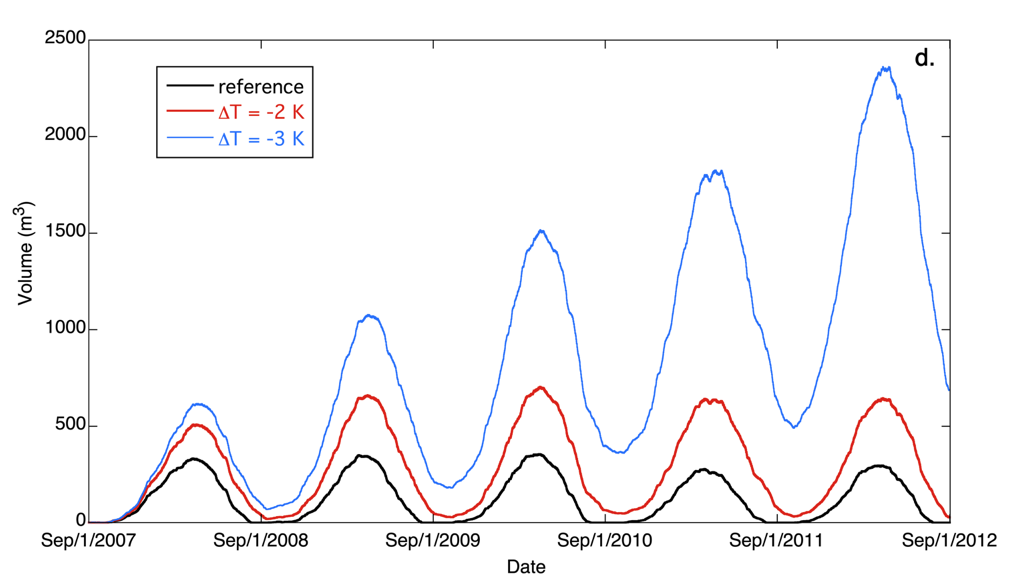
\includegraphics[width=\textwidth]{figs/PIR_evolution.png}
	\caption{The effect of a negative temperature perturbation. For $\Delta T = -3 \degree C$, the ice stupa does
		not disappear but grows from year to year.}
	\label{fig:PIR_evolution}
\end{figure}


\section{Interannual ice volume variability}
\label{sec:interannual}

\begin{figure}
	\centering
	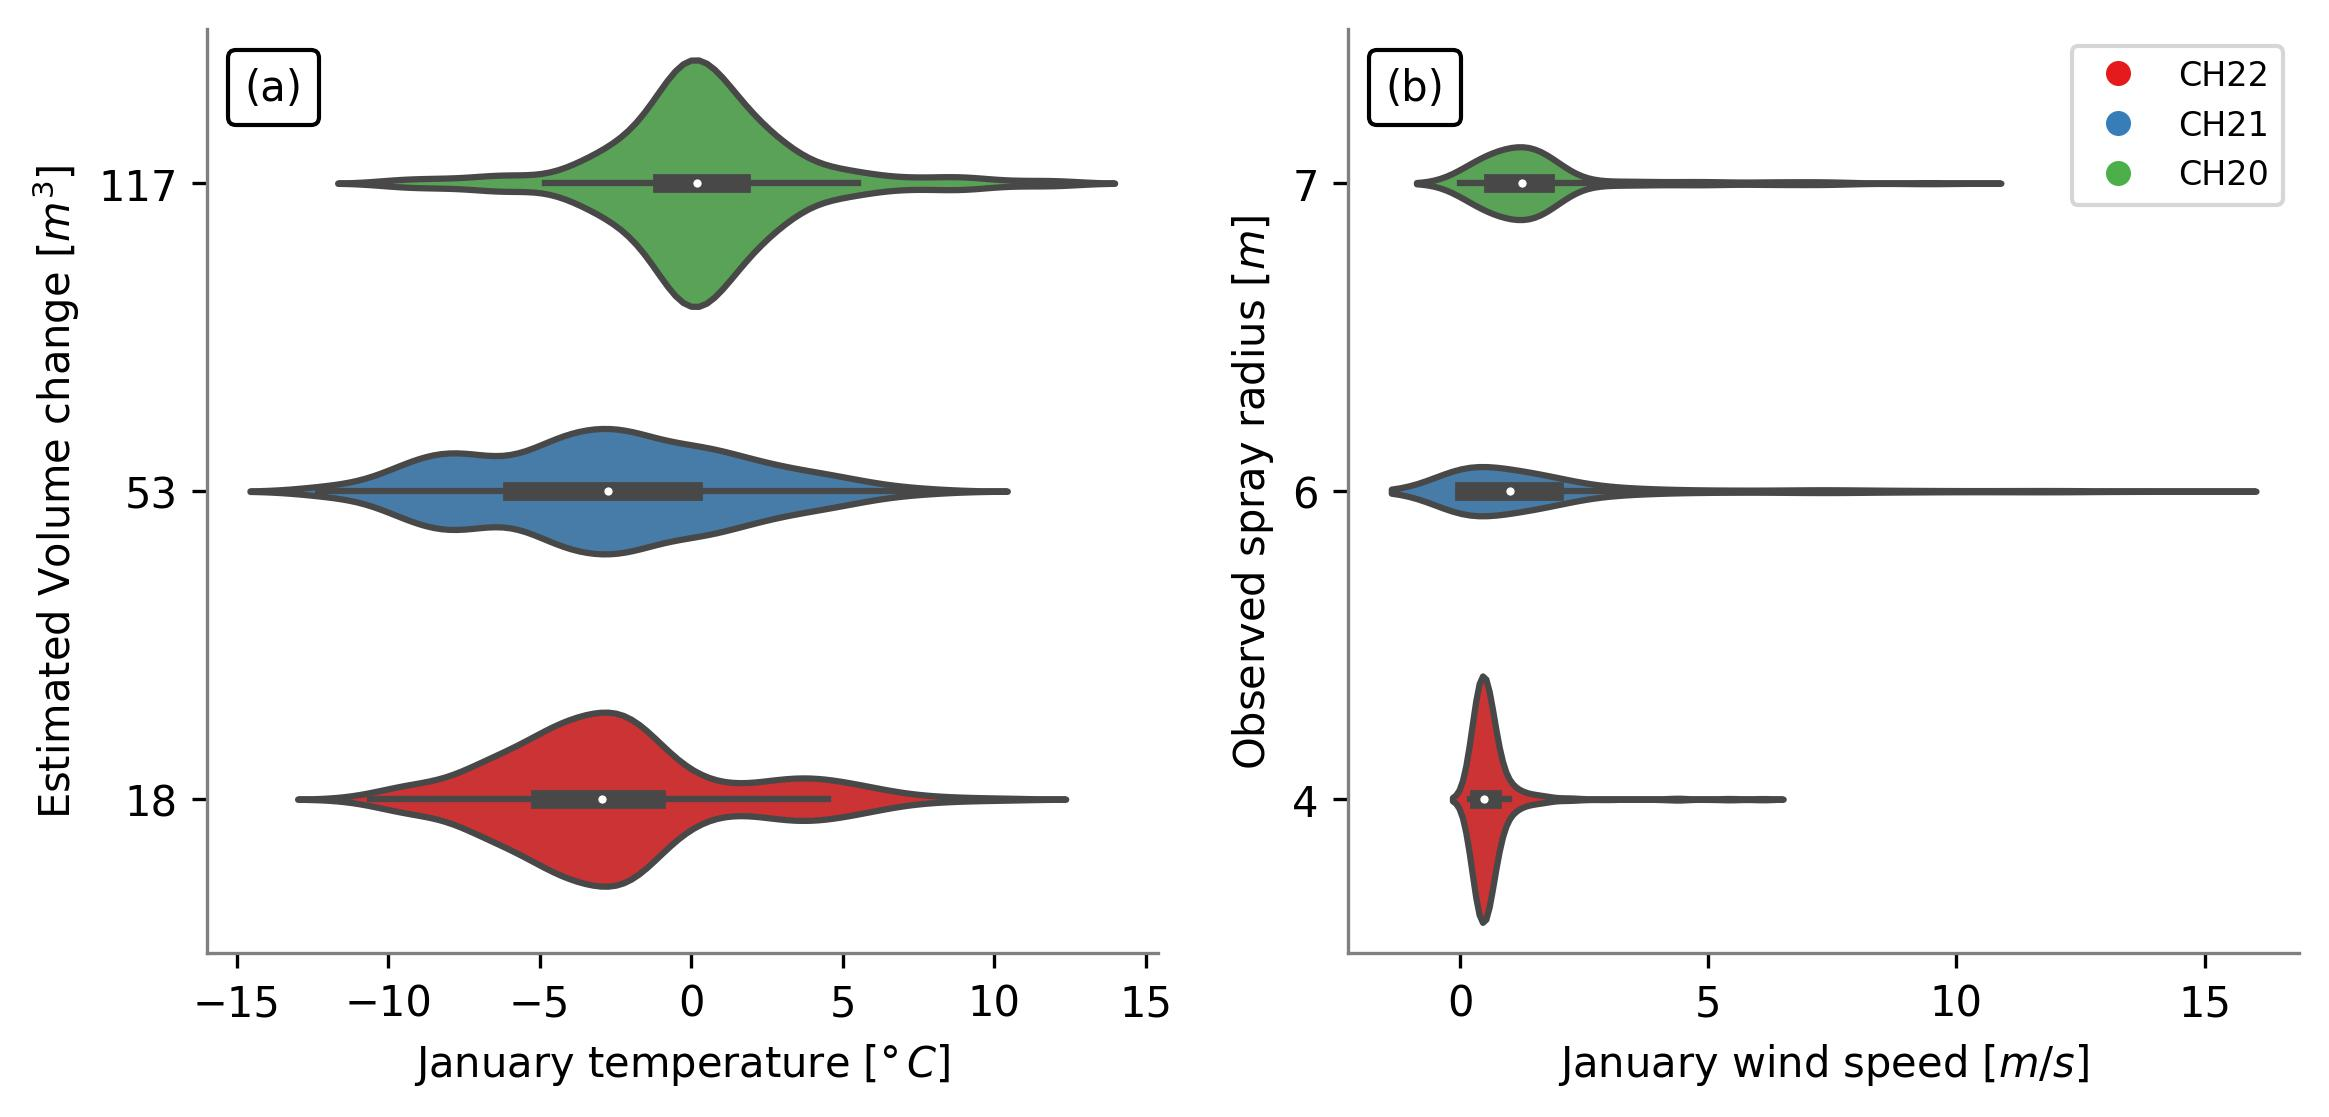
\includegraphics[width=\textwidth]{figs/CH_diffs.jpg}
	\caption{(a) Estimated volume change and temperature and (b) observed spray radius and wind speed
		during January for \ac{AIRs} built across three winters. }
	\label{fig:CH_diffs}
\end{figure}

\ac{AIRs} built in Switzerland across three winters (CH20, CH21, and CH22) show a decreasing trend in their ice volume
changes for the month of January. Contrary to expectations, this decreasing trend was not caused by increasing
temperatures but rather by decreasing wind speeds (Fig. \ref{fig:CH_diffs}). A process-based analysis revealed
that wind-driven redistribution of fountain water droplets could explain these differences (paper II). The influence of this process on
the fountain spray radius managed to generate \ac{AIRs} six times bigger in spite of temperatures being 3-$\degree C$
warmer (Fig. \ref{fig:CH_diffs} (b)).



   % INCLUDE: related work
\chapter{Heritage of ice reservoirs}

\cleanchapterquote{Before the artificial glacier, we struggled to get any barley. But now we can grow many
	crops, even potatoes, which need to be planted earlier in the spring, but sell for much more money.
}{Tashi Tundup}{(A 76 year old farmer in Ladakh)}

Climate warming has resulted in retreat and thinning of mountain glaciers
\citep{ipccCrossChapterPaperMountains2022}. This has implications for water availability in river basins that
have considerable glacierized areas in their headwaters, such as \ac{HMA}. Glaciers in HMA provide an important
gradual release of water that is used by many people locally and downstream for irrigation, drinking water and
hydropower. Climate change in this densely populated region may have serious consequences for glacier melt water
supply to the rivers \citep{immerzeelImportanceVulnerabilityWorld2020}. In this context, the development of
water storage technologies is crucial to ensure continued sustenance of cryosphere-fed irrigation networks.

People in mountains have a history of developing nature-based solutions to live in a dangerous and dynamic
environment, which will be invaluable to learn from for future adaptation and mitigation measures. One such
technology developed by communities in Ladakh are \ac{AIRs}. These strategies involve augmenting their glacial
ice reservoirs with man-made ones that provide supplementary irrigation during the spring.

\begin{figure}[htb]
	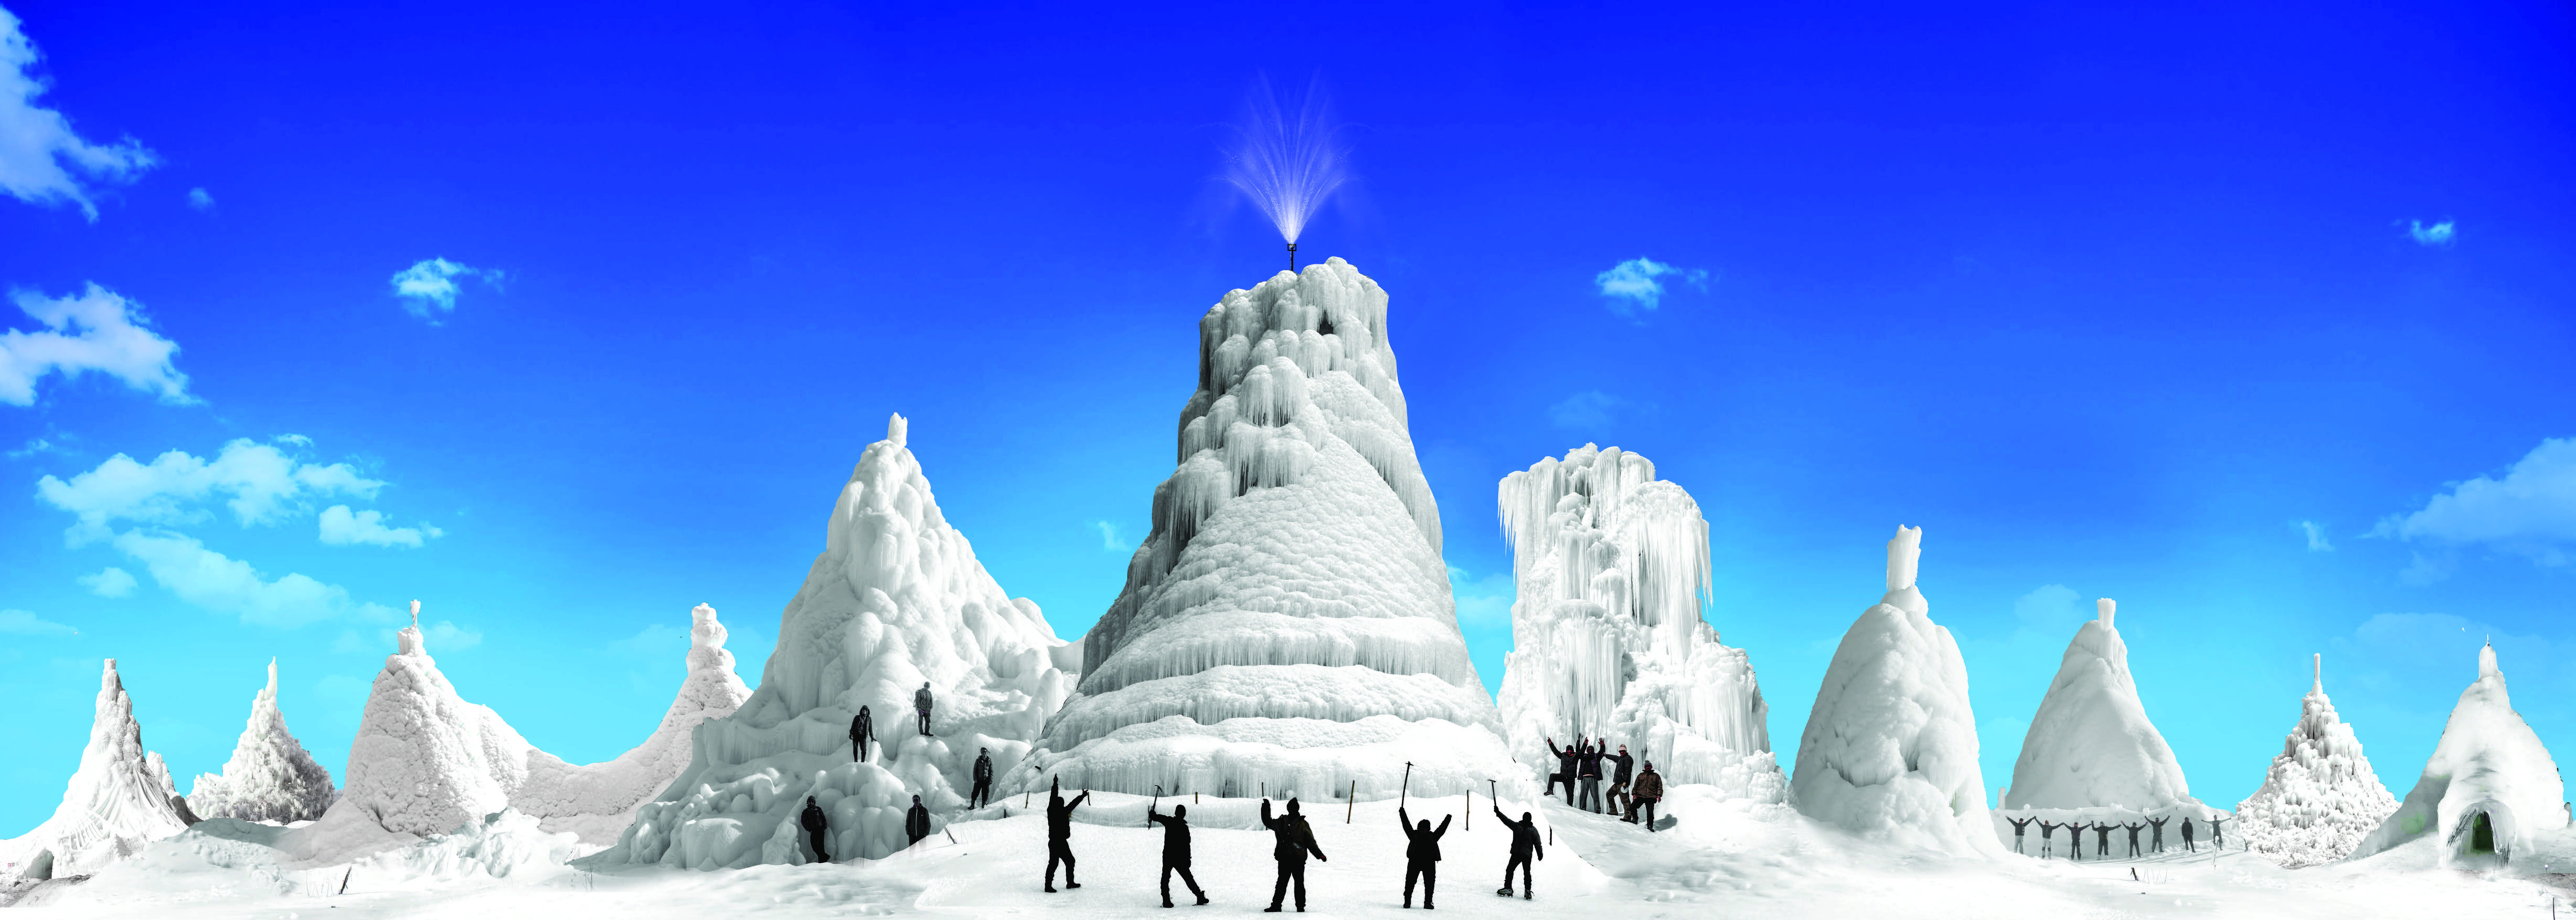
\includegraphics[width=\textwidth]{figs/AIRs_Ladakh}
	\caption{Compilation of AIRs built in different villages of Ladakh.}
	\label{fig:airs_ladakh}
\end{figure}

While these technologies have gained renewed attention as a strategy to increase water security, limited
scientific evidence exists about their potential hydrological contributions. AIR observations and investigations
date back to the mid-2000s \citep{tveitenGlacierGrowingLocal2007}. The vast majority have been published in the
2010s, mostly using qualitative methods. Because small-scale processes, complex feedbacks and non-linearities
govern their evolution, modelling the volume evolution of ice stupas is difficult and only feasible if backed up
with comprehensive datasets. Recent advances in glacial models and drones provide the opportunity to quantify
these surface processes using high-resolution data on volume changes of \ac{AIRs}. The main objective of the
thesis therefore was \textit{to increase understanding of volume dynamics of \ac{AIRs} in order to integrate
this tool in the water resource management strategy of mountain catchments}, with a specific focus on the
potential application of glacial models. This has been achieved by focusing on the following two specific
research questions:

\begin{enumerate}
  \item{What is the influence of construction location and fountain characteristics on ice stupa volume
    evolution?}
  \item{How can ice stupa fountain systems be engineered to reduce their water losses and maintenance efforts?}
\end{enumerate}

In this chapter, I discuss the main findings, integrate them in a broader perspective, point out limitations in
the methodology used, and provide recommendations and a future outlook.

\section{Conclusions}

\begin{figure}[htb]
  \centering
	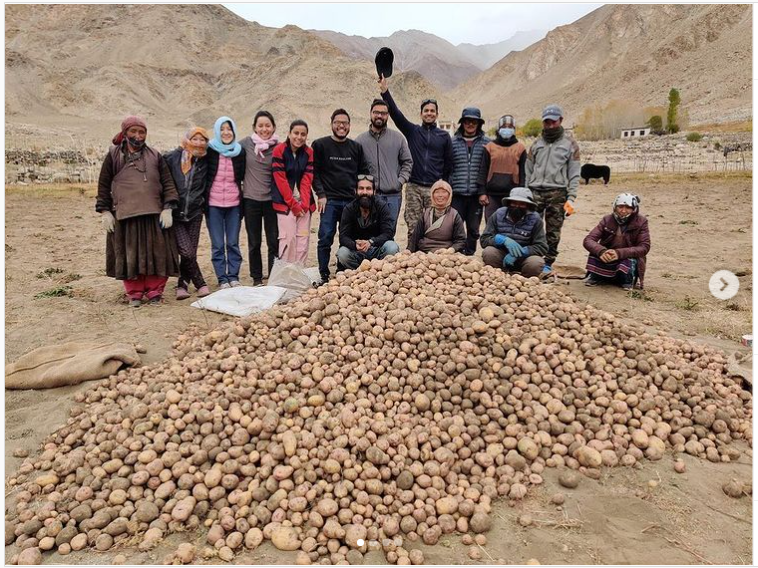
\includegraphics[width=8 cm]{figs/Kullum_potatoes}
	\caption{One of the deserted villages in Ladakh where AIR meltwater supported a harvest of 1300 kg of
		potatoes in October 2021. (Picture credits: Icestupa Project)}
	\label{fig:kullum_potatoes}
\end{figure}

In this thesis, we have developed three energy and mass balance models to simulate AIR evolution using data from
field measurements in Gangles, India and Guttannen, Switzerland. The use of these data sets, in combination with
the models, allowed for an accurate representation of the complex evolution that is typical of an AIR. We
studied the volume variation among eighteen AIRs and explained their corresponding magnitudes in terms of the
influence of the chosen location's meteorology, topography and the construction strategy used. Although the
approach is demonstrated on specific locations, it can be extended using the open-sourced models and global
reanalysis data sets to account for spatio-temporal meteorological influences of future locations on AIR's
volume dynamics. Our main conclusions are summarized below:

\begin{enumerate}

  \item The Indian construction site produced long-lasting AIRs with higher maximum ice volumes since it was
    colder, drier and less cloudy compared to the Swiss construction site. Thus, the AIR technology is ideally
    suited to serve as a water management strategy, especially in dry and cold mountain catchment such as in
    Central Asia or the Andes.

  \item Water losses of ice stupas were observed to be upto 80 \% due to excessive water input. However, the use
    of automated fountain scheduling strategies can lower their water consumption upto 10 times while reducing
    their maintenance requirements.

\end{enumerate}



\section{Challenges, recommendations and research outlook}

The studies presented in this thesis provide insights into the volume evolution of \ac{AIRs}. There are,
however, still various research gaps to overcome before \ac{AIRs} can be integrated into future water resource
management plans. In this section, I indicate important remaining scientific challenges and provide
recommendations and an outlook for future research.

\subsection{Metrics to judge site suitability}

We propose two sets of guidelines to identify future construction sites at a regional and a local scale. These
suggestions are guided by the different case studies presented in this thesis and field experiences in
Ladakh over the past six winters.

\subsubsection{Regional scale}

\begin{enumerate}

	\item Minimum median monthly temperature less than $0 \degree C$ to ensure sufficient freezing rate.
	\item Water supply with median discharge rate more than $2\, l/min$ to ensure sufficient water supply.
	\item Terrain slope between water source and site greater than 20 m every km to ensure sufficient
    gravitational head for fountain operation.

\end{enumerate}

\subsubsection{Local scale}

Given a valley or a region satisfying the above requirements, further selection of sites around the particular
water supply can be performed using the criterions below:

\begin{enumerate}
	\item Higher water source temperature to minimise risk of pipeline freezing events.
	\item Low daylight hours to decrease solar radiation induced melt.
	\item Higher altitude for higher freezing rates.
\end{enumerate}

\subsection{New ways to upscale irrigation water supply}

In this section, we describe two hypothetical ice stupa construction scenarios namely, historical and
futuristic. The historical scenario is a depiction of current construction efforts based on oral interviews and
field experience. The futuristic scenario is a depiction of how the tools developed in this thesis can transform
current construction efforts. The objective of both the scenarios is to maximize the meltwater available for
irrigation. Both these scenarios are motivated by the construction campaigns conducted in the Gangles valley of
Ladakh during the winter of 2019/20. This is the same valley where one of the study sites was located enabling
us to extrapolate some of the freezing rates and ice volume estimations from paper I (Fig.
\ref{fig:gangles_data}). We conservatively assume that the valley had a total water supply of around
$120\,l/min$, a winter duration of 4 months and the fountain was operational for only 8 hours per day for both
the scenarios. 

\begin{figure}[htb]
	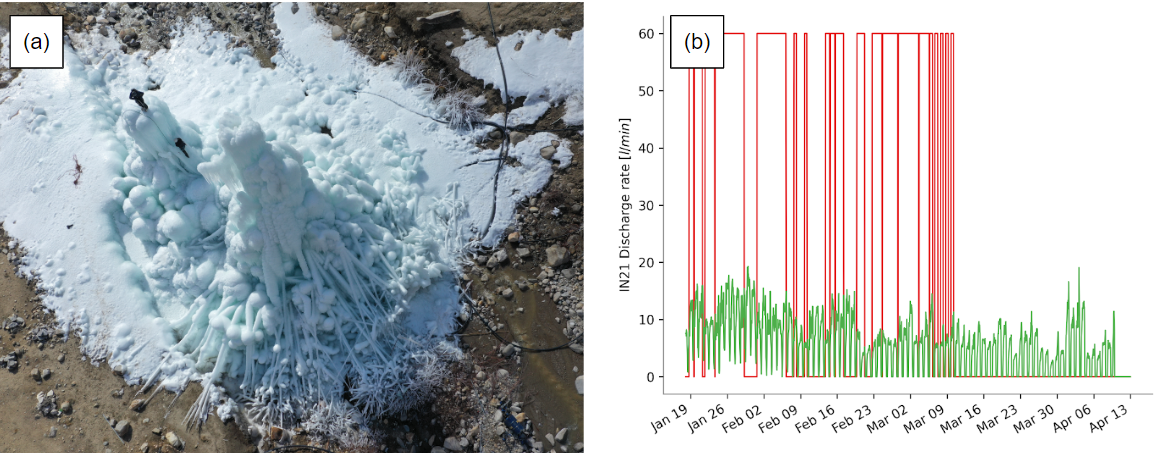
\includegraphics[width=\textwidth]{figs/gangles_data}

  \caption{(a) The IN21 ice stupa is a good example of the typical scenario of ice stupa construction (Picture
  credits: Norboo Thinles). (b) Its observed fountain discharge rate (red line) was interrupted several times
  due to pipeline freezing events. The discharge quantities used were also much higher than the estimated
  freezing rate (green line). }

	\label{fig:gangles_data}
\end{figure}

\subsubsection{Historical scenario}

In the historical scenario, only two fountains could be operated simultaneously using the available water
supply. This limited the construction period of each ice stupa to just two months. Moreover, pipelines froze
inside with ice blocks every few nights (Fig. \ref{fig:issues}). This resulted in two farmers investing more
than two months removing ice blocks and atleast thousand dollars repairing the fountain pipeline system to make
4 ice stupas. Assuming each ice stupa had a maximum ice volume similar to the one measured in Gangles (paper I:
Table 5), we expect the total ice volumes frozen in this valley to be around 3 million litres. This amounted to
a median irrigation water supply of around 44 thousand litres from mid-April to mid-June (based on measurements
shown in Section \ref{sec:icestupa_irr}).   

\begin{figure}[htb]
	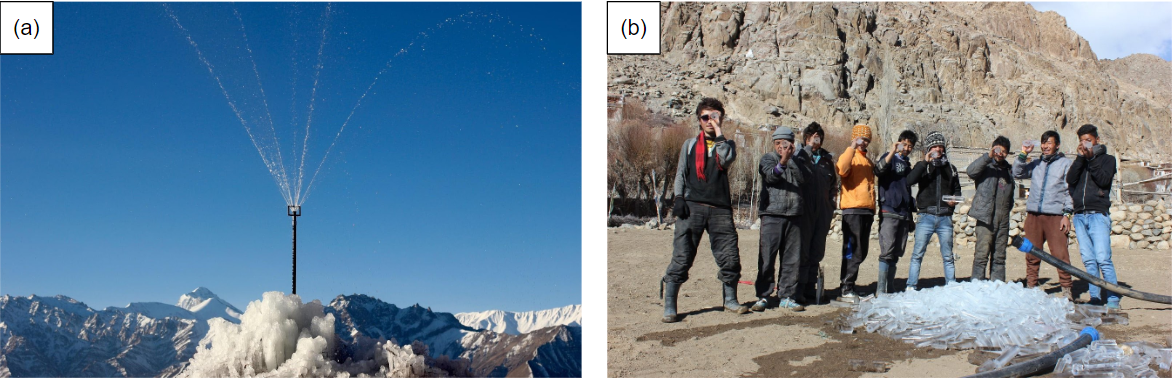
\includegraphics[width=\textwidth]{figs/construction_issues}

  \caption{The historical scenario of ice stupa construction is plagued with two major issues. (a) Fountains are
  supplied with too much water. (b) Fountain discharge is interrupted frequently due to ice blocks freezing
  inside the pipeline.}

	\label{fig:issues}
\end{figure}

\subsubsection{Futuristic scenario}

In the futuristic scenario, the automation system developed in the Technology chapter reduces the water
consumption of each ice stupa from $60\,l/min$ to $30\,l/min$. The additional cost to install such a system was
around thousand dollars. This enabled two farmers to build 8 ice stupas spending less than a week of effort
since there were no pipeline freezing events to deal with (Fig. \ref{fig:icestupa_valley}). The total ice
volumes frozen, however, resulted in more than 2 times higher irrigation water supply from mid-April to
mid-June.

\begin{figure}[htb]
	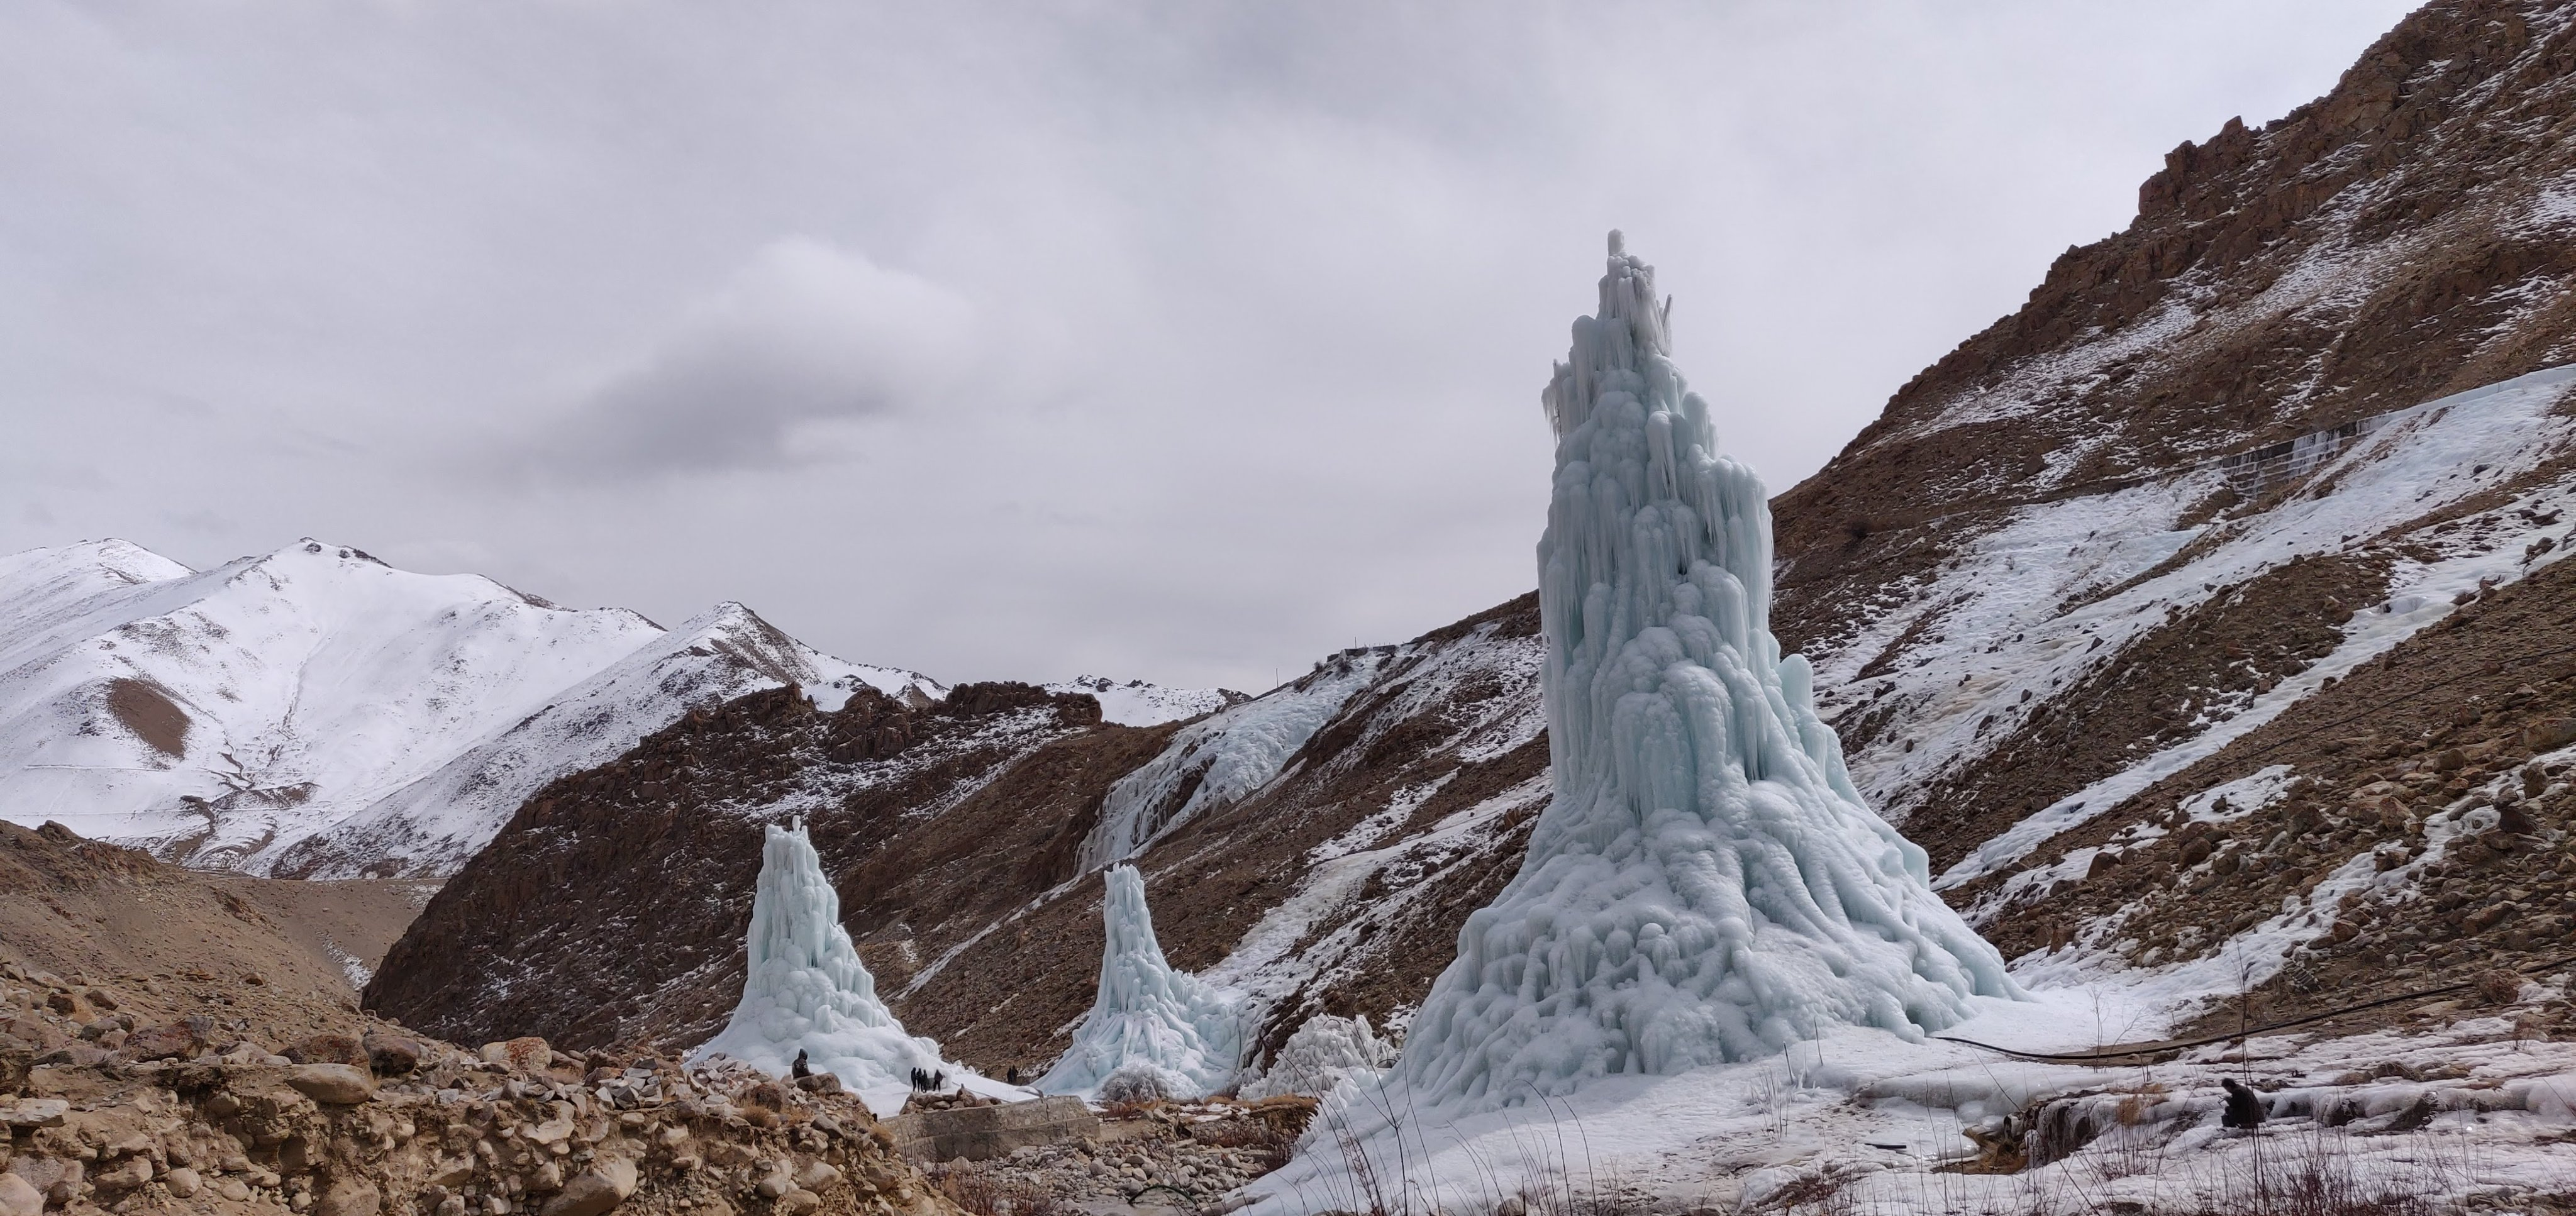
\includegraphics[width=\textwidth]{figs/icestupa_valley}

  \caption{More than a month of effort from a dozen farmers were required to build five ice stupas across the
  Gangles valley in the winter of 2019/20. Our research provides tools that two farmers can leverage to
  guarantee two times more winter water storage and reduce maintenance requirements to just a few days.}

	\label{fig:icestupa_valley}
\end{figure}

\subsection{The state of ice stupa technology}

The thesis shows one strategy that can improve the water-use efficiency of AIRs. We chose this strategy because
it enables the use of the AIR model in a simple and effective manner. However, all these construction strategies
are limited by the tools they use, namely the fountain and the pipeline. The fountain nozzle design is crucial
for increasing the ice volume obtained. However, no methodology currently exists to rank the several fountain
nozzles used for construction. An ideal pipeline configuration could make this technology cheaper and
maintenance free. However, optimization of the pipeline material and diameters is yet to be performed---despite
the time lost on pipeline freezing events and the potential cost reduction with cheaper pipeline materials and
sizes. Therefore, we strongly encourage the engineering community to get involved and push the limits of the
cost-effectiveness, size, and survival duration of artificial ice reservoirs.

\subsection{Quantification and development of ice terraces}

Although this thesis focuses on ice stupas, their ice volumes pale in comparison with ice terraces
\citep{nusserSociohydrologyArtificialGlaciers2019}. This is because ice stupas are limited by their fountain's
spray radius. However, ice terraces have no such limitations. Their thickness is only limited by the water
supply rate or meteorological conditions and they can occupy any construction area provided. But despite this, ice
stupas are the preferred method of ice harvesting due to their longer survival duration and reduced construction
effort.

With a suitable redesign of the automation hardware, automated construction strategies can also be applied on
ice terraces. Such a construction strategy can potentially compound their size every consecutive winter with
minimal maintenance requirements. Therefore, future research direction should aim to answer the following
questions:

\begin{itemize}

	\item How can ice terrace construction systems be engineered to reduce their water losses and maintenance
	      efforts?

\end{itemize}

The methodology developed in this thesis should also apply for such an analysis.


\subsection{Adaptation potential of glacierized catchments with AIRs}

Vanishing glaciers, natural hazards (like inundations, mudflows, and landslides), decreasing river discharge,
drying springs, next to shifts in precipitation patterns are apparent climate change impacts which affect
glacierized catchments.

In the Peruvian Andes, both water scarcity (low-flow water risk) and glacial lake outburst floods (high flow
water risks) could have important impacts on local population, infrastructure and economic activities
\citep{motschmannIntegratedAssessmentsWater2020}. For example, the estimated loss in annual wheat output due to
reduced glacial runoff would be to the tune of 18 million USD even in the low emission scenario of Quillcay catchment
of Peru \citep{motschmannLossesDamagesConnected2020}. Similarly, in the Stok catchment of Ladakh, glacial ice
reserves have shrunk by more than 18 \% in the past 16 years, leading to a decline in crop productivity
\citep{sohebSpatiotemporalQuantificationKey2022}.

AIRs can already buffer against low flow water risks in certain catchments. For example, ice
terraces in nearby valleys have been measured with areas up to 19 \% of the Stok glacier (0.8 $km^2$). With further technology
development, AIRs can also be used to mitigate high flow water risks. The glacial lakes of the Andes and
Himalayas can be siphoned to form AIRs in scale that last perpetually. Such AIRs can compound over the years to
become another source of perennial water supply for the respective catchments.


\subsection{Model development}

The COSISTUPA model developed in section \ref{sec:Cosistupa} should be used for future estimations for AIR
volume. This model needs to be extended so that it can account for future climate variability and produce
accurate meltwater predictions. Modelling the future is fundamentally different from simulating the past: In the
past the model serves as a tool for interpreting and best exploiting field measurements - and can be directly
constrained by them. Models for the future must understand climate variability to be able to yield realistic
projections. Almost all methodological steps in the modelling of future AIR runoff are subject to possible
enhancements, always bearing in mind that we will only know whether the effort led to an enhanced or even a
worsened performance, when we're old...

Model development is an art where subjective choices seek a balance between a model's simplicity and its
accuracy. Below we detail some of these choices and recommend strategies that shift this balance towards further
model accuracy.

\subsubsection{Quality and quantity of calibration and validation data sets}

The methodology used to acquire the radius, area and volume of \ac{AIRs} (Appendix \ref{sec:drone_method}) from
each drone survey has several drawbacks. The calibration and validation process used has an inherent temporal
and spatial bias due to the following subjective choices:

\begin{itemize}
	\item \textbf{The number and timing of the drone surveys}. For example, among the five surveys of IN21 AIR, most of them were
	      conducted around early March when the AIR volume was near its maximum whereas the seven surveys of the CH21
	      location were more evenly spaced out in comparison. This observation bias occured due to logistical issues
	      in conducting measurements in regular intervals.

	\item \textbf{The meteorological conditions under which surveys were performed.} Particularly, precipitation events reduce DEM quality since
	      they create uniform snow surfaces over \ac{AIRs}. These surfaces do not allow the identification of features
	      that can be used to extract the radius and area of the AIR.

\end{itemize}

Thus, the quality of AIR validation is severely limited by the high uncertainties attached with the drone
processing methodology.

This limitation can be overcome by extending the model validation set using two measurement approaches. First,
we suggest measuring daily AIR meltwater quantities. Accuracy of this validation method depends on the wind
speeds of the location but can be improved if the terrain is made waterproof and oriented so that most of the
AIR runoff can be collected. 

Second, we suggest conducting \ac{GPR} surveys. \ac{GPR} is sensitive to subtle changes in the properties of ice
layers. This makes it a powerful tool to image the internal structure of ice structures. The basic principle of
a pulsed \ac{GPR} system is to send an electromagnetic signal into the ground and to record the signal
reflections as a function of their two-way travel time. Partial reflections of the electromagnetic wave recorded
as internal reflection horizons (IRH) occur at vertical discontinuities in the dielectric material. From polar
studies, IRH are known to coincide with variations in density and liquid water content
\citep{forster2014extensive}. Therefore, \ac{GPR} can be a crucial method to calibrate and validate spatial
density and volume variations of \ac{AIRs}.


\begin{figure}[htb]
  \centering
	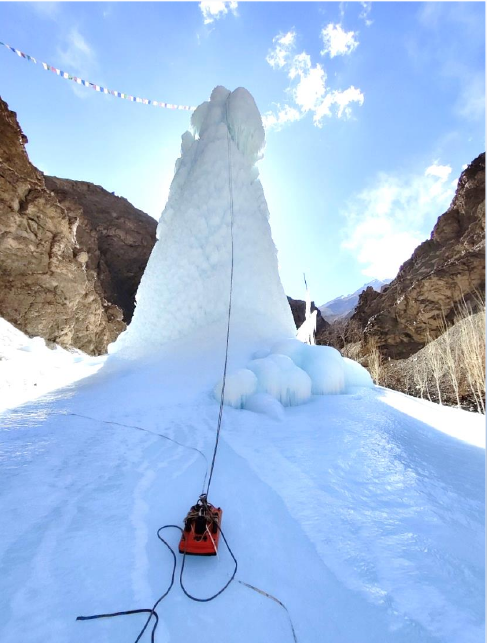
\includegraphics[width=8 cm]{figs/gpr_survey}
  \caption{Portable \ac{GPR}s were carried across the surface of \ac{AIRs} to produce the associated datasets. (Picture credits:
  Shijay Projects)}
	\label{fig:gpr_survey}
\end{figure}

\ac{GPR} surveys were already conducted on four ice stupas in March 2020 (Fig. \ref{fig:gpr_survey}). However,
these data sets remain unused. They can be downloaded at \citet{balasubramanian_suryanarayanan_2022_7056646}.

\subsubsection{Albedo parametrization}

The albedo parametrization illustrated by Equation \ref{eqn:alb} had to be modified to accomodate the fountain
discharge events. Little knowledge is available to understand the decay of albedo due to such events. Therefore,
a simplistic approach of increasing the decay rate by a constant factor is used. However, the value of this
factor is chosen without any basis on measurements. Field based albedo measurements are required to better
parametrize the effect of water spray on the surface albedo decay rate.

\subsubsection{Turbulent heat flux parametrization}

The method used to calculate turbulent heat fluxes by \citet{garrattAtmosphericBoundaryLayer1992} assumes that
these fluxes are acting over a uniform planar surface. This leads us to use the exposure/roughness parameter
$\mu_{cone}$ as a correction factor. However, equation \ref{eqn:mu} about $\mu_{cone}$ is no more than an educated guess. It
is hard to base estimates of this parameter on information in the literature. Many studies have been carried out
on the effect of obstacles on atmospheric boundary layer flow (e.g. trees), but always in an ensemble setting,
looking at the bulk effect of an ensemble of obstacles. We deal with a case of a single obstacle in open
terrain, and we are confident that the roughness of the surface and the exposure will lead to larger turbulent
fluxes.

\subsubsection{Fountain quantification}

Contrary to our model assumptions, the parameters used to define the fountain were not independent. The fountain
height, fountain aperture diameter (both ignored in this analysis), discharge rate, water temperature and spray
radius were related through the trajectories of the water droplets.

All our models require the fountain spray radius to be provided as input. This is a significant limitation
since these models are very sensitive to the spray radius parameter. Moreover, spray radius is not only determined
by the fountain characteristics but also due to wind-driven redistribution, refreezing and melting events across
the AIR perimeter. The same fountain was observed to produce different spray radius corresponding to different
winters for the Swiss experiments. Further discussion on this can be found at Section \ref{sec:interannual}.

During the IN21 experiment, snow formation was observed, indicating that the fountain water droplets have the
potential to freeze before deposition on the AIR surface. Modelling such processes would require modelling the
conduction, convection and nucleation processes that all droplets undergo during their flight time. Therefore, a
proper quantification of the fountain is much more complex and requires a closer look at the correlation of the
fountain parameters amongst themselves and with the meteorological parameters.


\section{Final thoughts}

Glaciers provide an important buffer for highly seasonal precipitation regimes
\citep{kaserContributionPotentialGlaciers2010}. Under the currently available climate change projections it is
expected that glacial mass loss will continue in future decades, and that several smaller glaciers will continue
to disappear completely \citep{rabatelCurrentStateGlaciers2013}.

These trends stress the importance of increased water storage capacity for glacierized catchments as a pathway
for climate adaptation. Because of the challenges and cost related to traditional storage efforts, AIRs can be a
better tool to adapt against reduced glacial runoff. In order to quantify their adaptation potential, it is
necessary to understand the changing dynamics of AIR melting, but also map how their meltwater contributes to
current and future water use. While the spatiotemporal dynamics of AIR melt are increasingly well understood and
documented in this thesis, major uncertainty remains on how their meltwater contribution propagates through the
hydrological system and compares against the total discharge of mountain catchments.

Future research needs to determine which catchments can benefit most from the supplementary water supply
provided by these ice harvesting technologies and flag off the urgent climate action required to increase their
water security.


% In arid and semiarid regions, in particular, it is estimated that between 50 \% and 90 \% of freshwater
% resources originate from mountain catchments \citep{messerliMountainsWorldVulnerable2004}. During drought
% conditions in the tropical mountain regions, glacial meltwater is used by upto 3.92 million domestic users and
% to irrigate 2096 $km^2$ of land \citep{buytaertGlacialMeltContent2017}.

% Identifying which combination of interventions optimizes the return-on-investment and adaptive capacity in view
% of future climate uncertainty remains a challenge, especially in arid mountain regions. 

% The implementation of adequate adaptation strategies will need to respond to these changes,
% as well as a growing anthropogenic demand for water \citep{buytaertWaterCitiesImpact2012}.

% \subsection{Shape parameterization}
%
% The \ac{RMSE} between the drone and the model estimates of the surface area for the IN21, CH21 and CH20 \ac{AIRs}
% were 69 \%, 25 \% and 65 \% of the maximum area of the respective \ac{AIRs}. There are two rough assumptions
% leading to such a large error, assuming a conical shape and assuming a constant spray radius.
%
% Better quantification of the surface area can be achieved by assuming AIR cross section to be a Gaussian curve
% rather than a triangle.
%
% Better quantification of the spray radius can be achieved by modelling the projectile motion of fountain water
% droplets using wind speed values and fountain characteristics as illustrated in Section \ref{sec:interannual}.
     % INCLUDE: conclusion
\pagestyle{empty}				% no header or footers
\chapter{Papers on ice reservoirs}
% \section{First author papers}

\section{Paper I}
\vfil\null
\huge{\textbf{Influence of Meteorological Conditions on Artificial Ice Reservoir (Icestupa) Evolution}}

\bigskip
\large{Balasubramanian, S., Hoelzle, M., Lehning, M., Bolibar, J., Wangchuk, S.,
  Oerlemans, J., and Keller, F. \par  Frontiers in Earth Science 9 (February 23, 2022): 771342.
doi:10.3389/feart.2021.771342.}

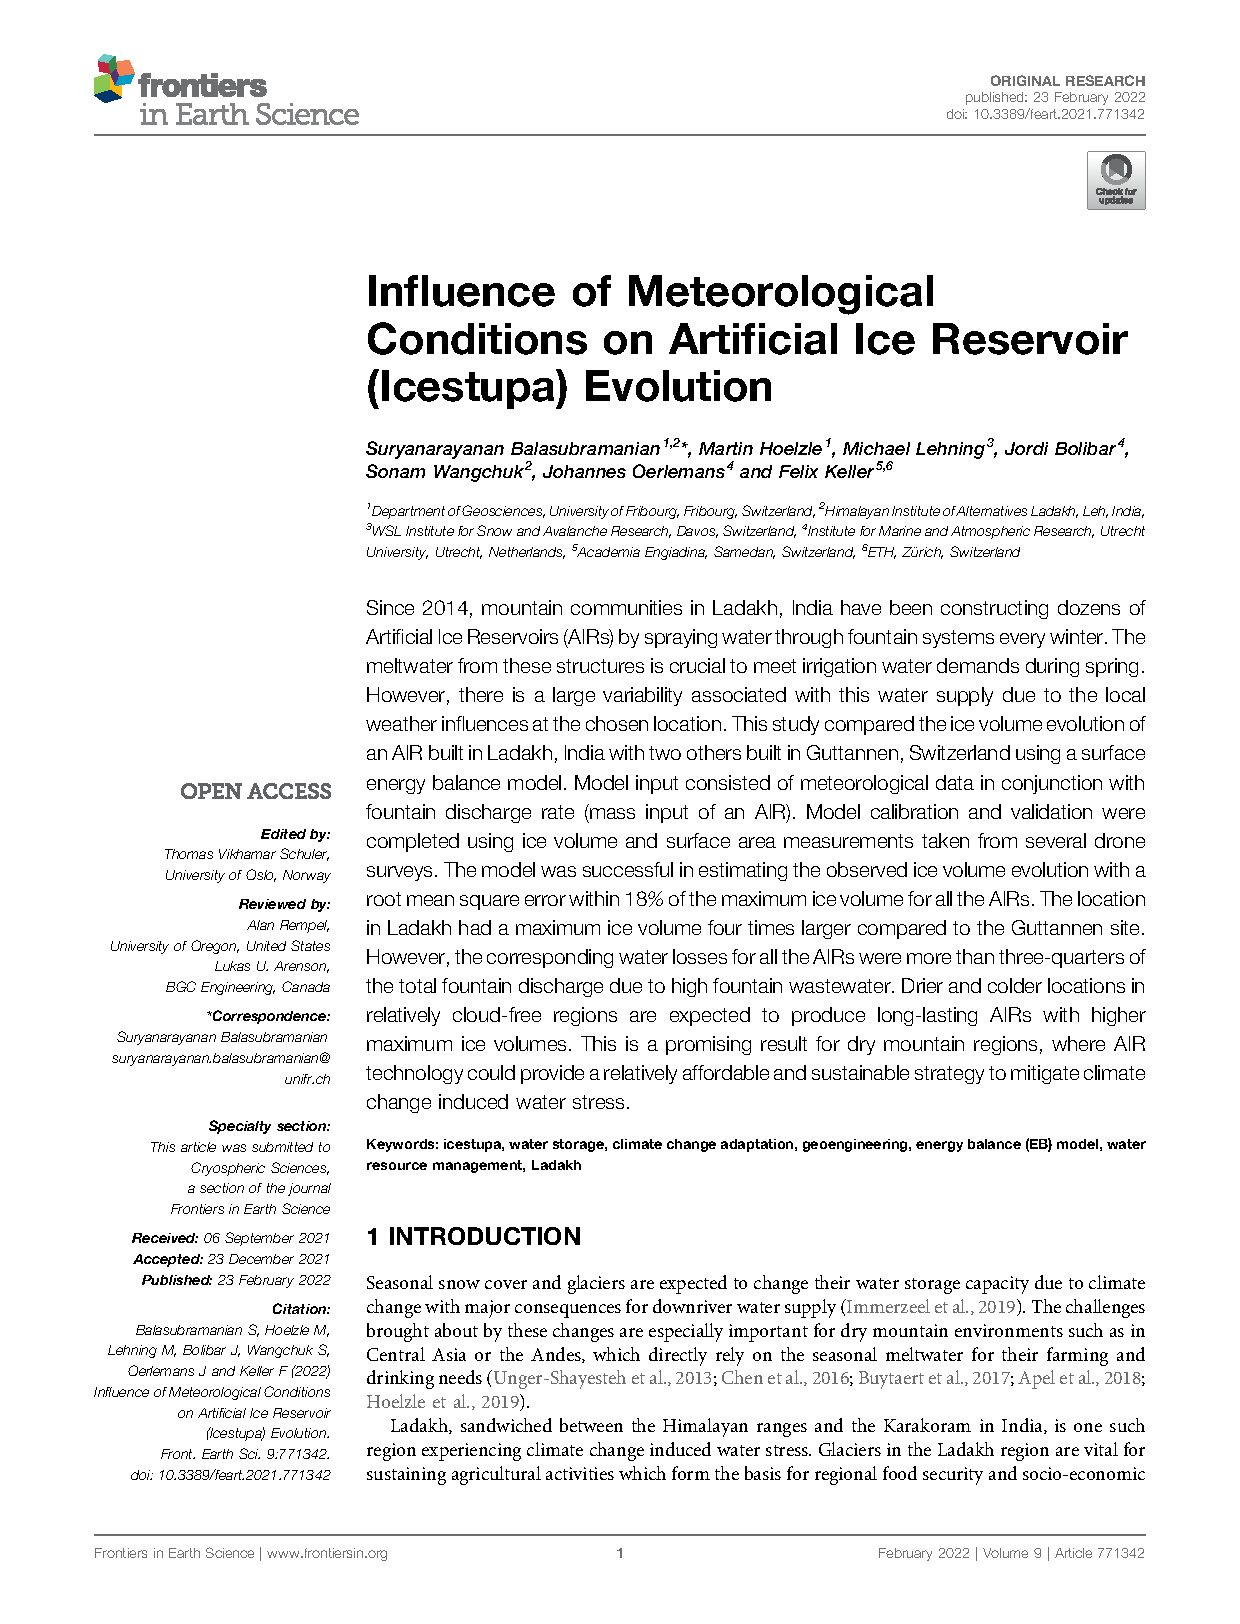
\includepdf[pages=-,pagecommand={},width=\paperwidth, scale=10]{content/papers/paperI (optimized).pdf}

\section{Paper II}
\vfil\null
\huge{\textbf{Improving water-use efficiency of artificial ice reservoirs (Icestupas) through weather-sensitive fountain scheduling
strategies}}

\bigskip
\large{Balasubramanian, S., Hoelzle, M., and Waser, R. \par  Frontiers in Earth Science 9 (February 23, 2022): 771342. doi:10.3389/feart.2021.771342.}

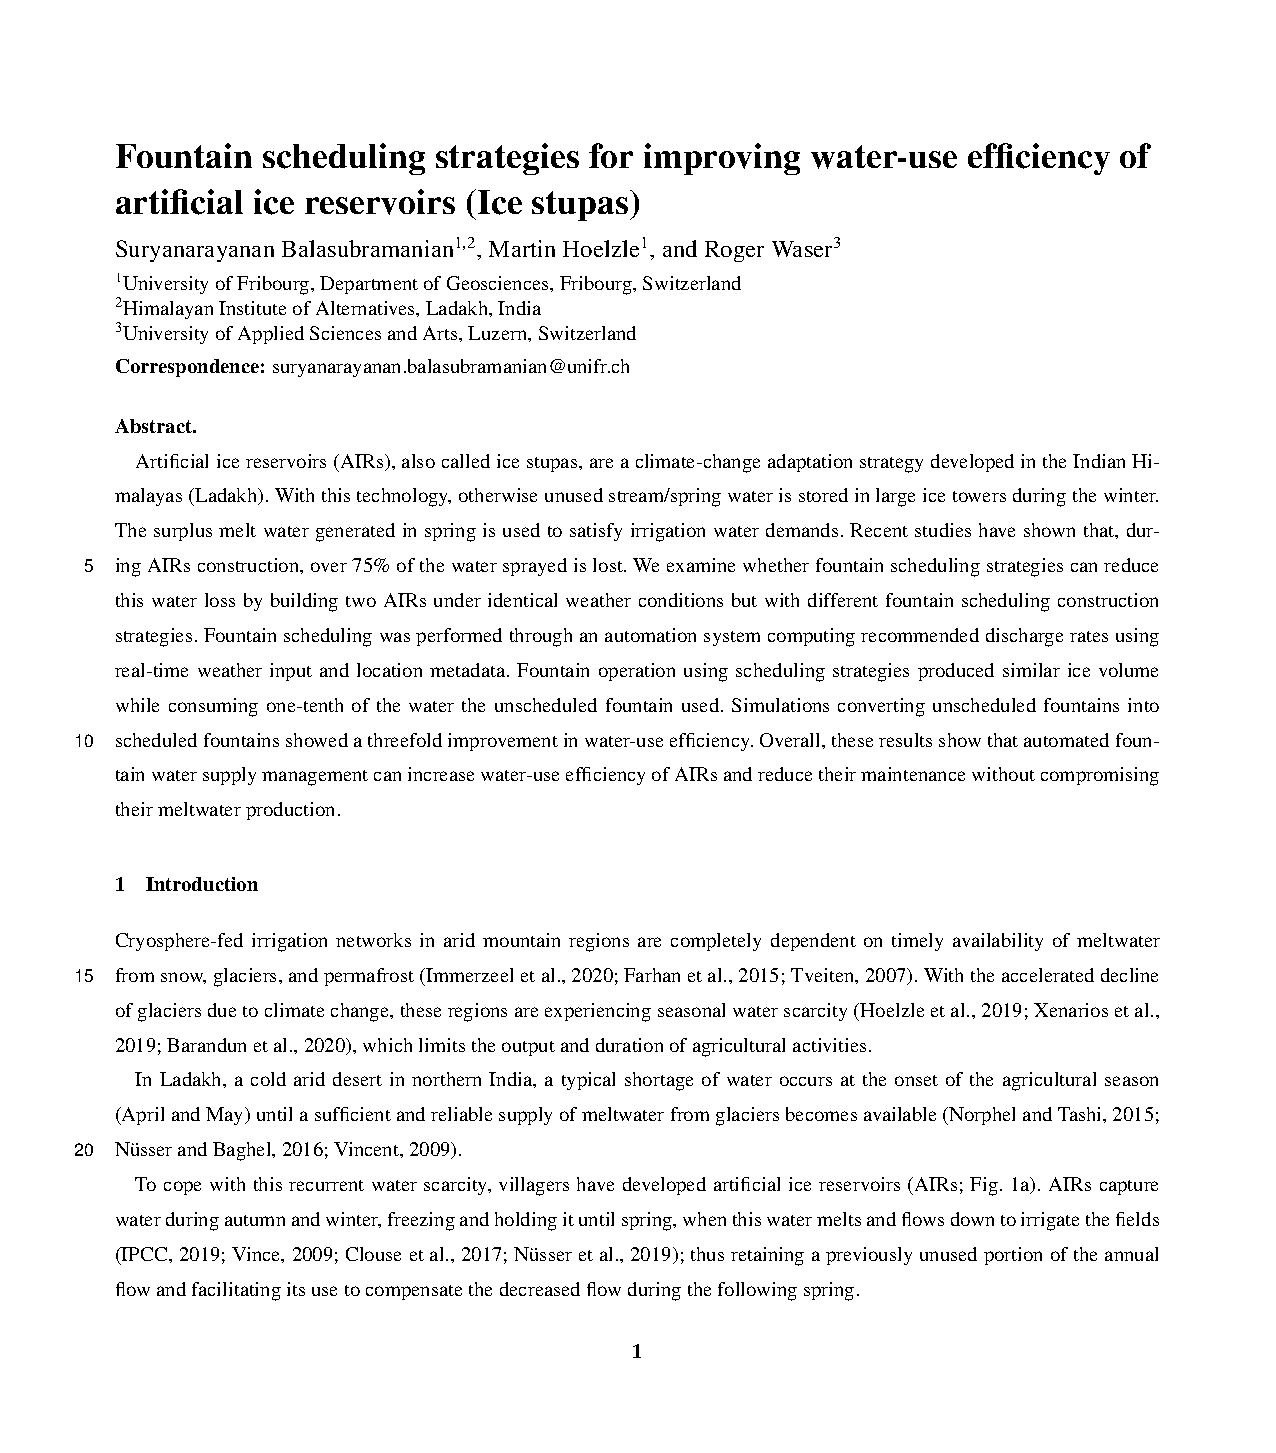
\includepdf[pages=-,pagecommand={},width=\paperwidth, scale=10]{content/papers/paperII (optimized).pdf}

% \section{Co-authored papers}
\section{Paper III}
\vfil\null
\huge{\textbf{Brief communication: Growth and decay of an ice stupa in alpine conditions – a simple model driven by energy-flux observations over a glacier surface}}

\bigskip
\large{
Oerlemans, J., S. Balasubramanian, C. Clavuot, and F. Keller. The Cryosphere 15, no. 6 (2021): 3007–12. doi:10.5194/tc-15-3007-2021.
  }

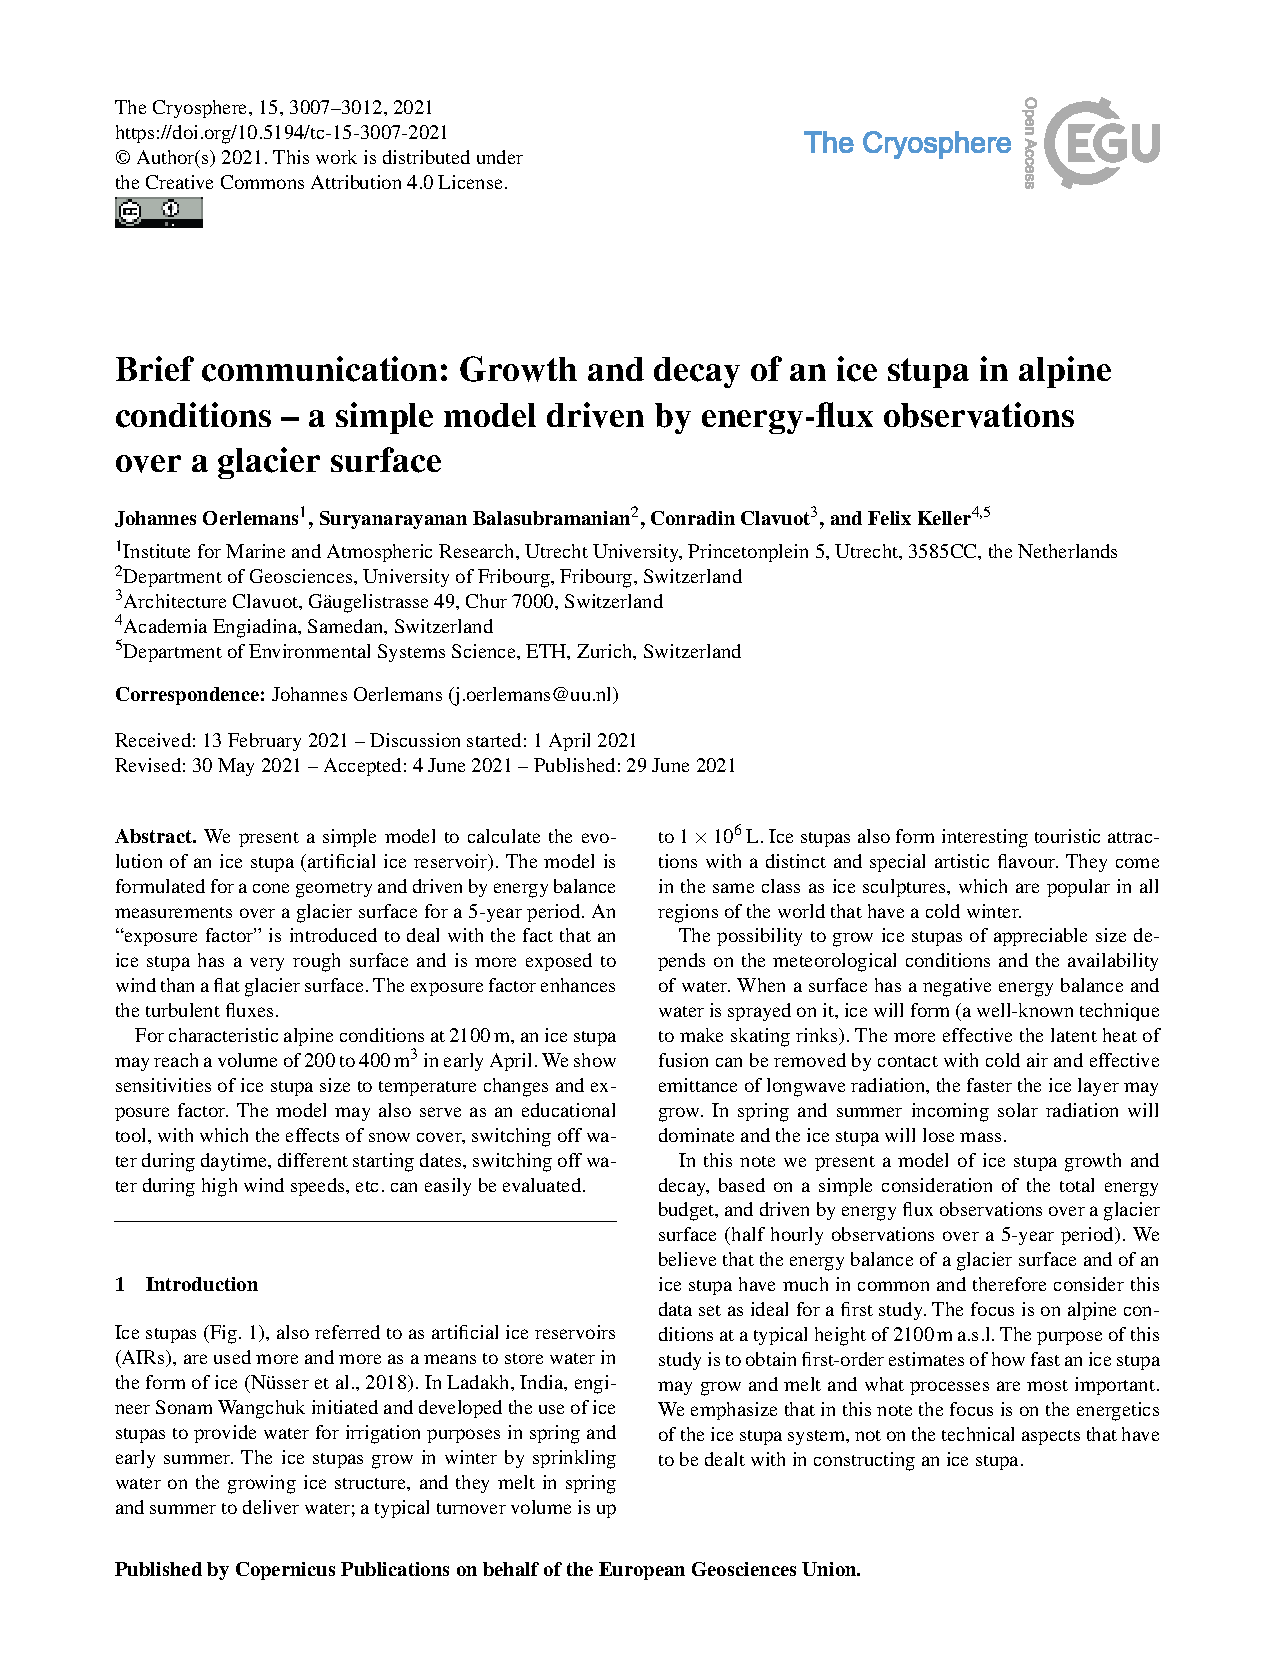
\includepdf[pages=-,pagecommand={},width=\paperwidth, scale=10]{content/papers/paperIII (optimized).pdf}



\appendix\cleardoublepage
\chapter{Appendix}
\label{sec:appendix}

\section{Paper I}
\vfil\null
\huge{\textbf{Influence of Meteorological Conditions on Artificial Ice Reservoir (Icestupa) Evolution}}

\bigskip
\large{Balasubramanian, S., Hoelzle, M., Lehning, M., Bolibar, J., Wangchuk, S.,
  Oerlemans, J., and Keller, F. \par  Frontiers in Earth Science 9 (February 23, 2022): 771342.\par
doi:10.3389/feart.2021.771342.}

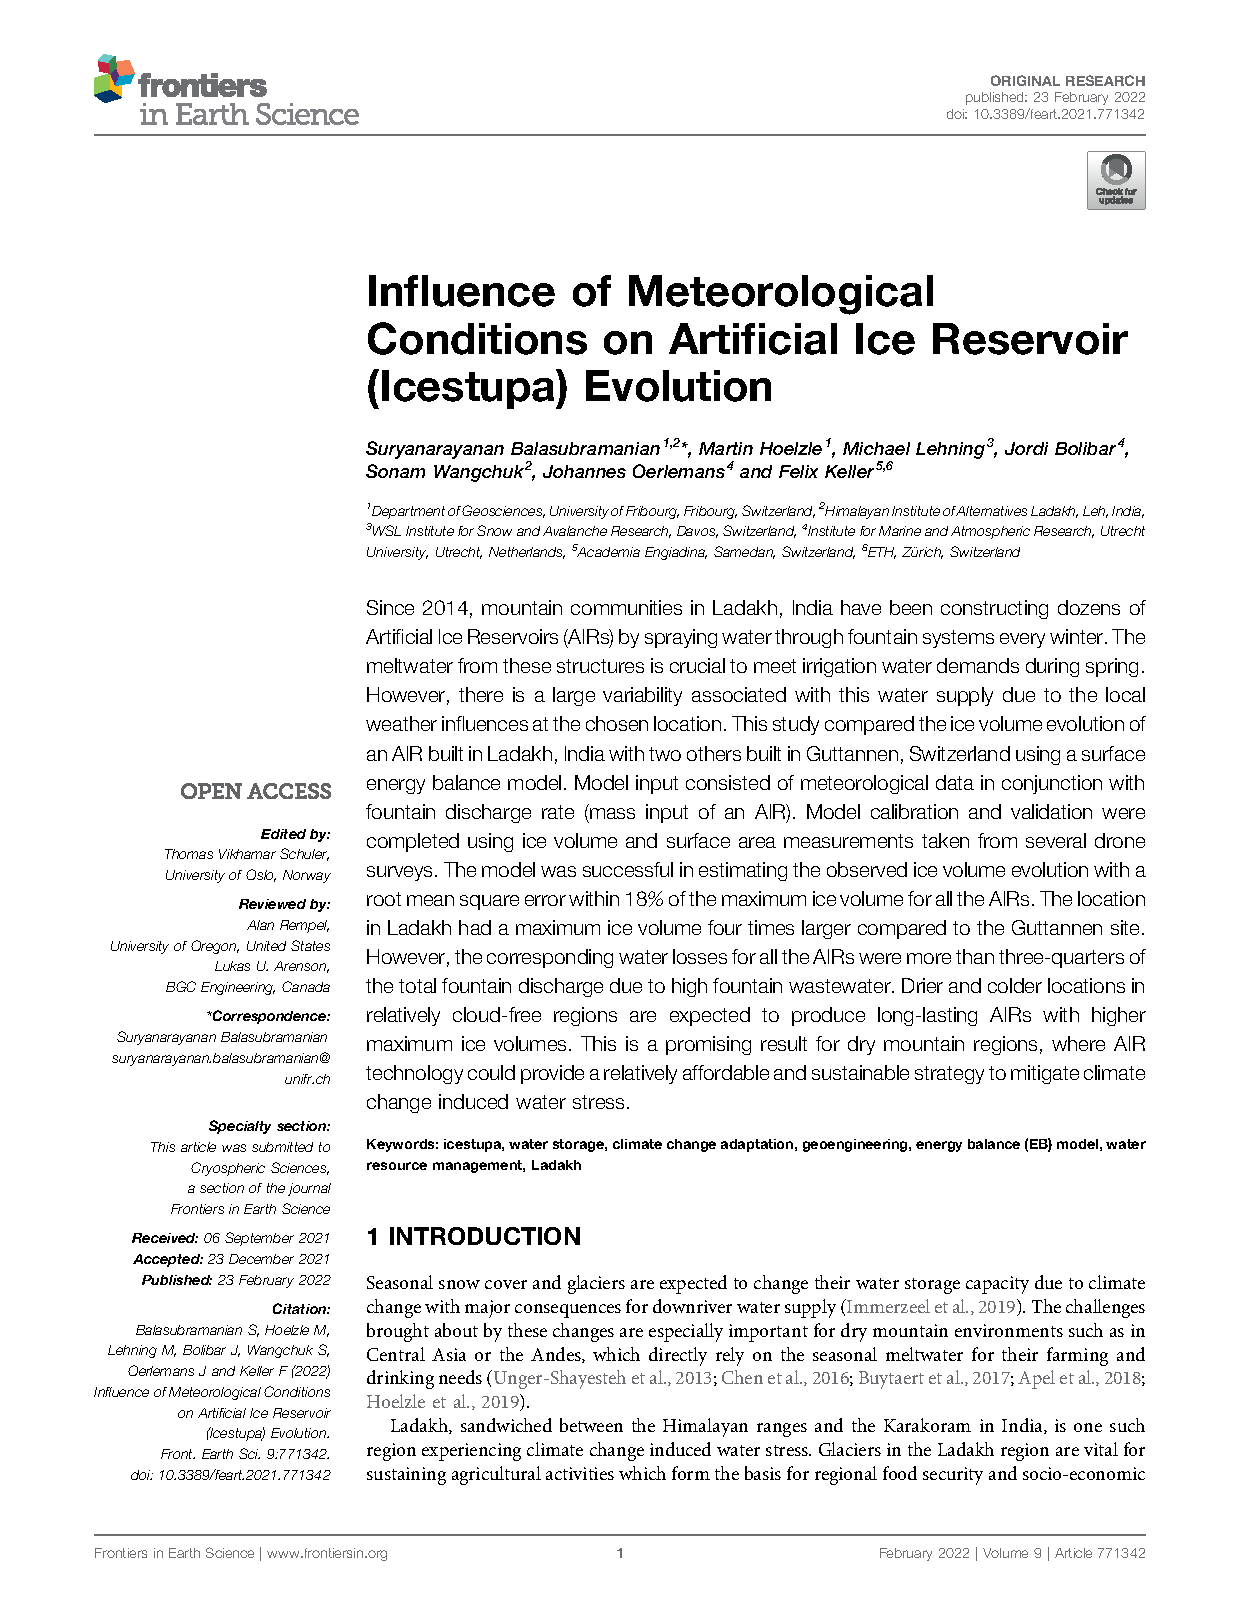
\includepdf[pages=-,pagecommand={},width=\paperwidth, scale=10]{content/papers/paperI.pdf}

\section{Paper II}
\vfil\null
\huge{\textbf{Fountain scheduling strategies for improving water-use efficiency of artificial ice reservoirs (Ice stupas)}}

\bigskip
\large{Balasubramanian, S., Hoelzle, M., and Waser, R. \par  Cold Regions Science and Technology (October 30,
2022) \par doi:10.1016/j.coldregions.2022.103706 }

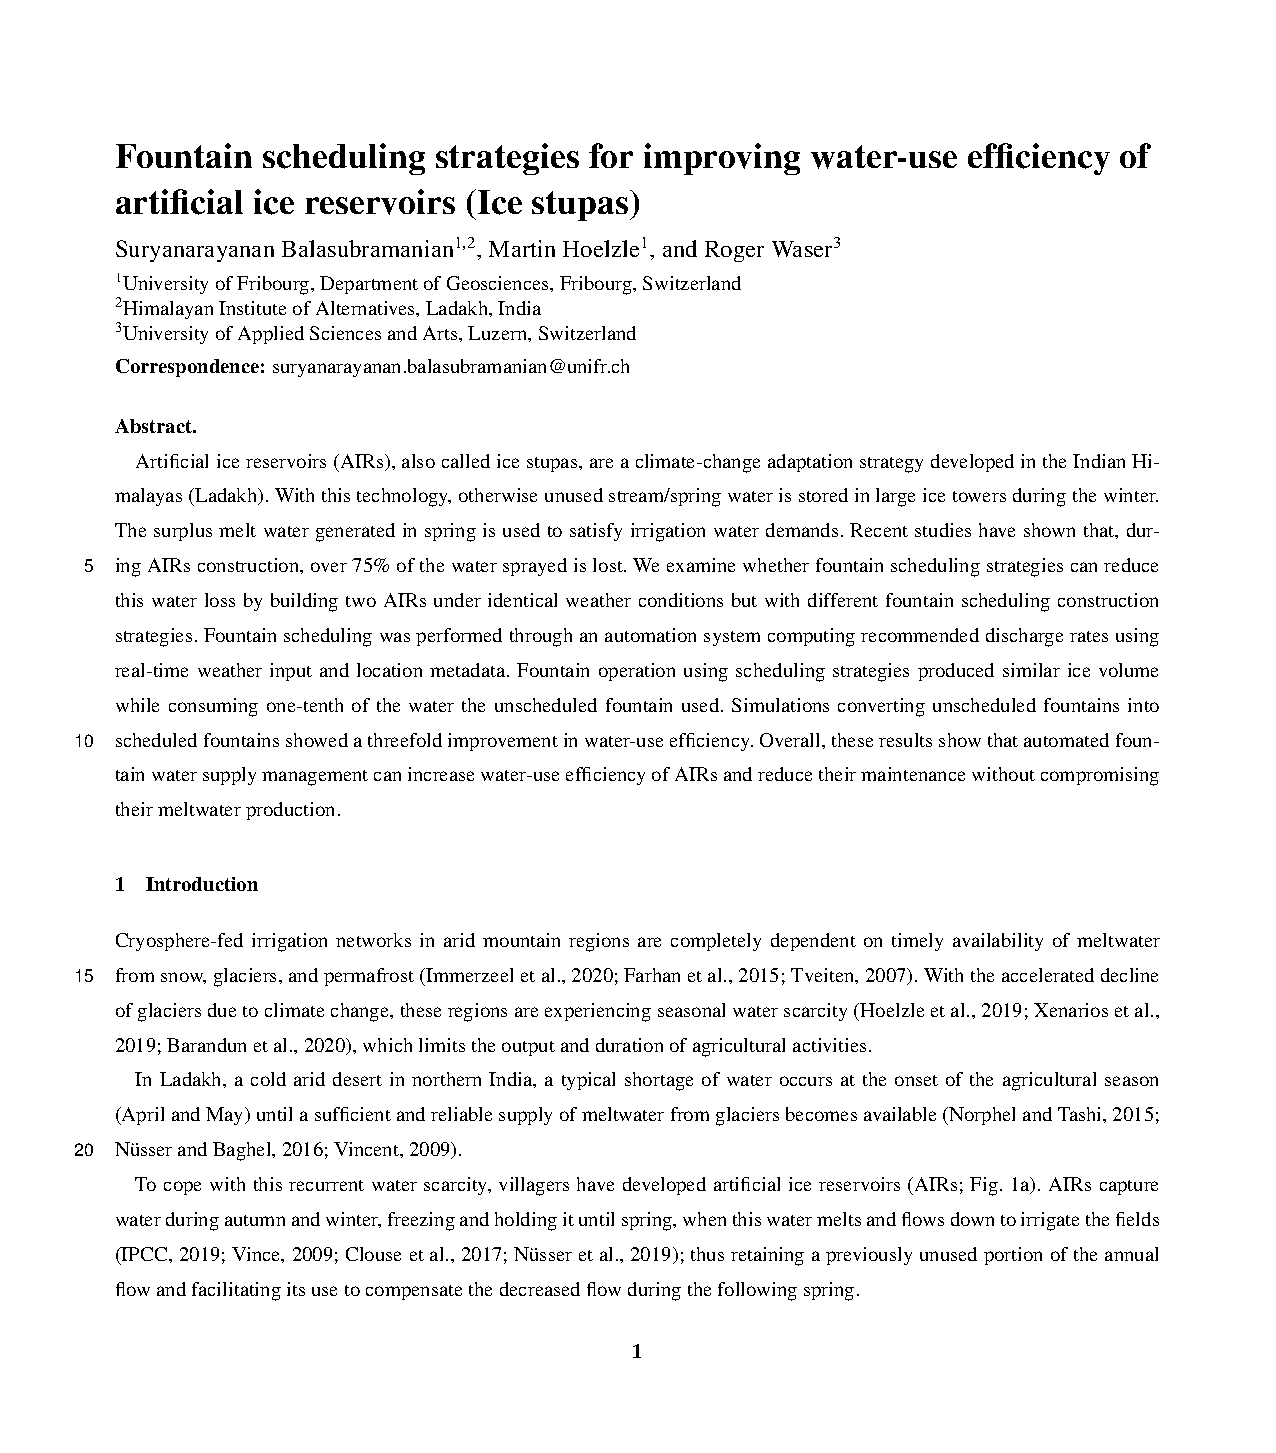
\includepdf[pages=-,pagecommand={},width=\paperwidth, scale=10]{content/papers/paperII.pdf}

% \section{Co-authored papers}
\section{Paper III}
\vfil\null
\huge{\textbf{Brief communication: Growth and decay of an ice stupa in alpine conditions – a simple model driven by energy-flux observations over a glacier surface}}

\bigskip
\large{
Oerlemans, J., S. Balasubramanian, C. Clavuot, and F. Keller. \par The Cryosphere 15, no. 6 (2021): 3007–12.
\par doi:10.5194/tc-15-3007-2021.
  }

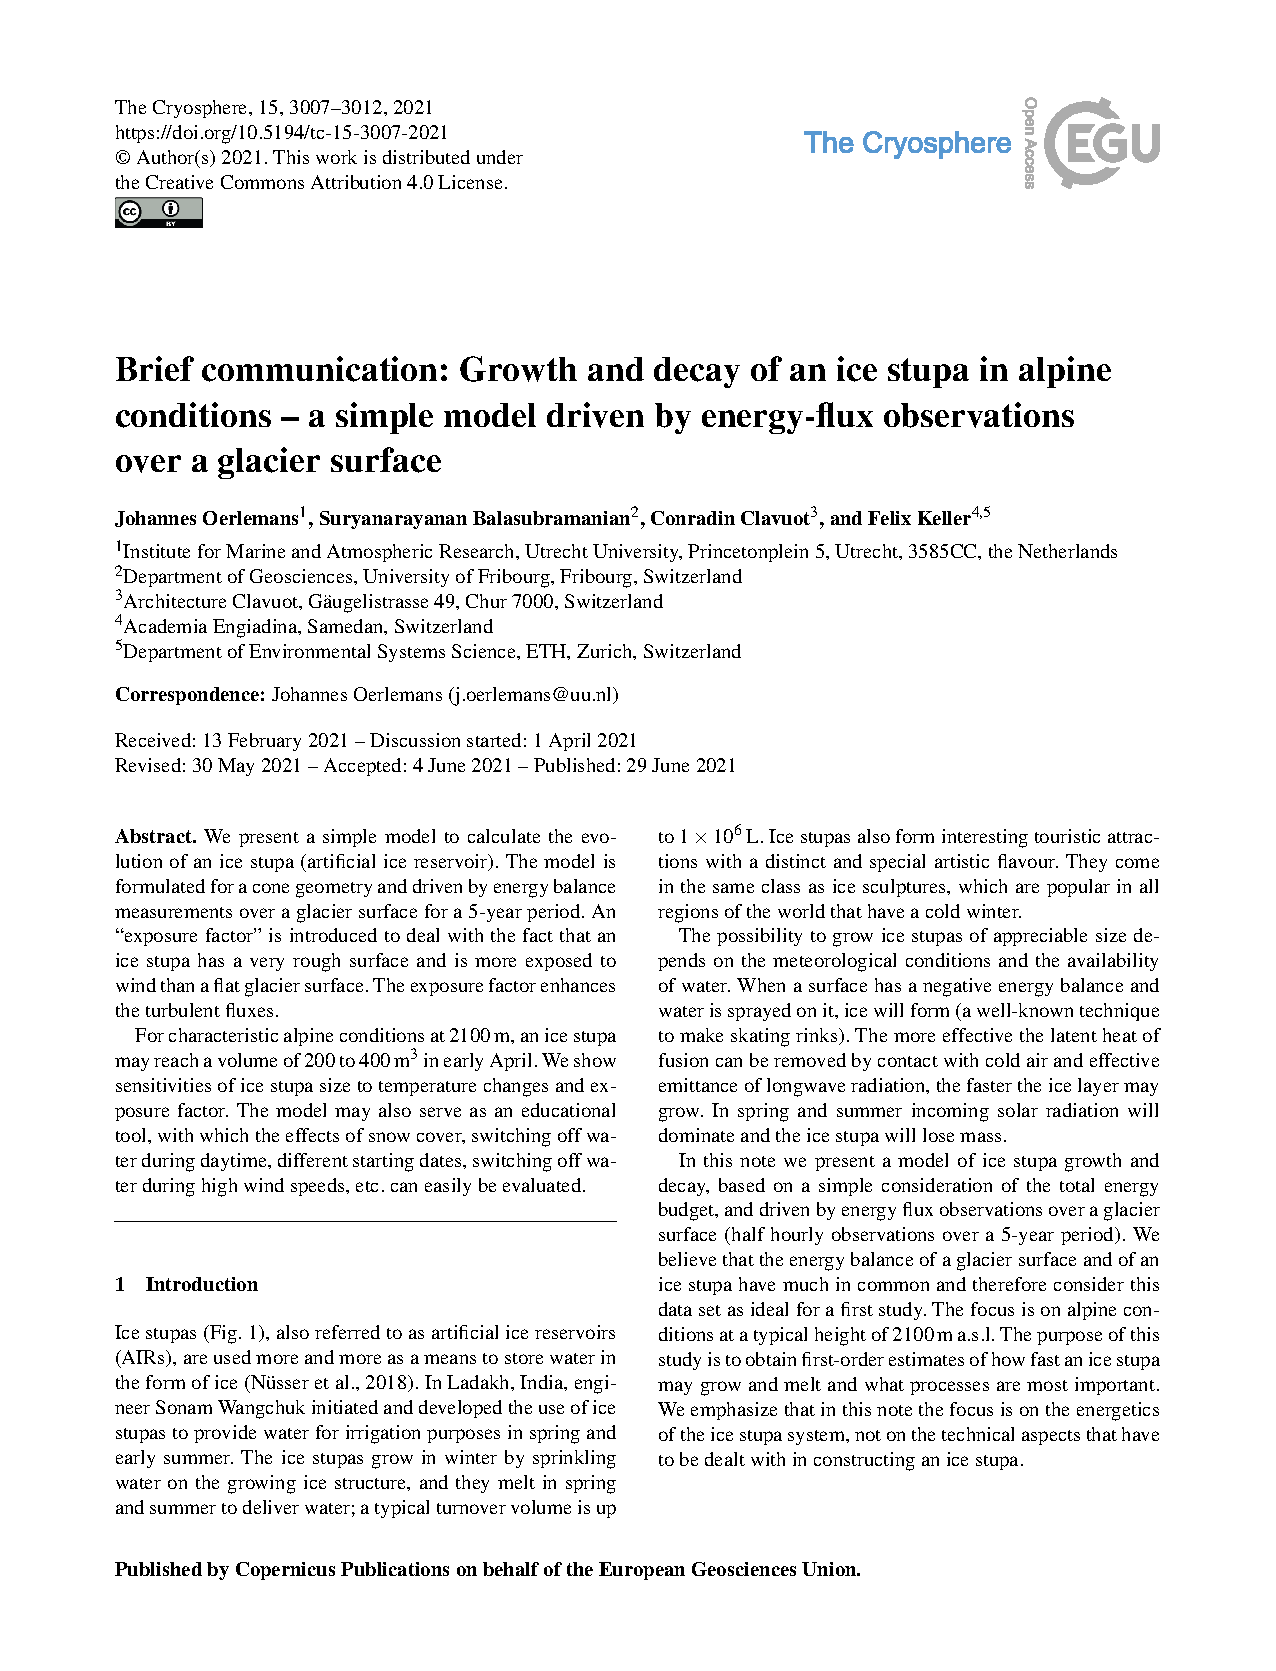
\includepdf[pages=-,pagecommand={},width=\paperwidth, scale=10]{content/papers/paperIII.pdf}

\section{Drone surveys and their processing methodology}
\label{sec:drone_method}

The drone flew along a predefined flight course and took photographs at set time intervals. The
position and altitude of the drone at the exposure stations, which were obtained by the built-in integrated
position and orientation system (POS, composed of a global positioning system and inertial measurement units),
were recorded in JPEG pictures. In the present work, we adopted a three-step workflow, as implemented in the
commercial software package Pix4Dmapper version 4.6.4 (\cite{pix4dsaPix4DmapperUserManual2020}). A short summary of this workflow is
described below:

\begin{figure}
	\begin{center}
		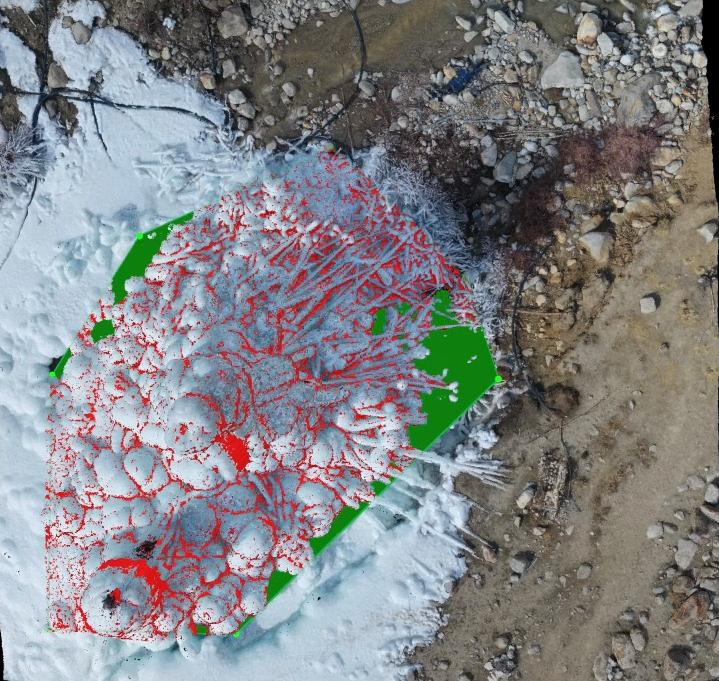
\includegraphics[width=12 cm]{figs/pix4d.jpg}
	\end{center}
	\caption{Digital elevation map of Indian \ac{AIR} constructed from the drone survey on March 3, 2021. The green
		area represents the area bounded by the marked perimeter, and the red area represents gaps in the point cloud
    that were filled to compute the associated volume.
	}
	\label{fig:DEM}
\end{figure}

(1) Initial processing: This process generates a sparse point cloud with the structure-from-motion algorithm
(\cite{turnerAutomatedTechniqueGenerating2012}). First, it searches for and matches key points in the photos which present certain overlapping
areas using a feature matching algorithm (e.g., the scale-invariant feature transform (SIFT) algorithm, which can
detect key points in photos under different views and illumination conditions;
\cite{loweDistinctiveImageFeatures2004}). Second, the approximate locations and orientations of the camera at
each exposure station are reconstructed with the internal parameters (focal length, coordinates of the principal
point of the photograph) and external parameters (i.e., POS data). A sparse point cloud is created.

(2) Point cloud densification: In this step, the multiview stereo technique is applied to achieve a higher
point cloud density than that in the previous step (\cite{furukawaAccurateDenseRobust2010};
\cite{molgStructurefromMotionUsingHistorical2017}). Thus, the spatial resolution of the products can be
increased, and an irregular network for the next step can be created (\cite{kungACCURACYAUTOMATICPHOTOGRAMMETRIC2011}).

(3) \ac{AIR} delineation: Ice radius, area, and volume are the three final products. Perimeter is manually marked
on the point cloud by identifying the \ac{AIR} boundary (Fig. \ref{fig:DEM}). For the Indian location, identical rock features were identified
near the ice boundary to mark as vertices of this perimeter. For the Swiss \ac{AIR}, no such feature was available due
to snowfall, so instead, the perimeter was marked by identifying the ice and snow boundary.

Temporal and spatial uncertainty is associated with this process. Weather conditions influence the quality
of each drone survey to various degrees. Moreover, since ice/snow surfaces do not present many identifiable features, few
feature points can be detected and matched in the vicinity of the \ac{AIR}. Thus, a high uncertainty of
$\pm 10 \%$ is attached for all the \ac{AIR} observations to accommodate for this.

\begin{table}[htb]
  \centering
  \caption{List of all \ac{AIRs} studied in Ladakh. Adapted from \citet{mariagruberIceStupasLadakh2022}.}
	\label{tab:Ladakh_AIRs}
	\begin{tabular}{|lllll|}
    \hline
    \textbf{Location}     & \textbf{Winter season} & \textbf{Altitude [$m\,a.s.l.$]} & \textbf{
    Radius [$m$]} & \textbf{Volume [$m^3$]} \\ \hline
    Igoo & 2019/20 & 4209 & 23 & 4918  \\
    Karith & 2019/20 & 3710 & 12 & 1451  \\
    Karith 2 & 2020/21 & 3692 & 5 & 1133  \\
    Lamso & 2019/20 & 3859 & 7 & 615  \\
    Lamso 2& 2020/21 & 3863 & 6 & 420  \\
    Nang& 2019/20 & 3897 & 13 & 1601 \\
    Phyang& 2019/20 & 3916 & 19 & 5182 \\
    Sandoo& 2019/20 & 3773 & 10 & 1483 \\
    Shara& 2019/20 & 4288 & 18 & 7936 \\
    Gangles& 2020/21 & 4072 & 9 & 602 \\
    Apati& 2020/21 & 3840 & 6 & 351 \\
    Mulbeck& 2019/20 & 3451 & 11 & 1887\\
    Nang& 2019/20 & 3897 & 13 & 1601\\
    Skurbuchan& 2019/20 & 3023 & 9 & 956\\
    Takmachik& 2019/20 & 3032 & 13 &1265\\
    Takmachik 2& 2020/21 & 3052 & 10 &1604\\
    Tarchit& 2020/21 & 3962 & 17 &2363\\
    Patherak& 2020/21 & 3899 & 10 &770\\
    Kullum& 2020/21 & 3907 & 7 &328\\ \hline
	\end{tabular}
\end{table}


% \section{Ground penetrating radar surveys}
% \label{sec:gpr}
%
% \ac{GPR} is sensitive to subtle changes in the properties of ice layers, making it a powerful tool to image the
% internal structure of ice structures. The basic principle of a pulsed \ac{GPR} system is to send an
% electromagnetic signal into the ground and to record the signal reflections as a function of their two-way
% travel time. Partial reflections of the electromagnetic wave recorded as internal reflection horizons (IRH)
% occur at vertical discontinuities in the dielectric material. From polar studies, IRH are known to coincide with
% variations in density and liquid water content \citep{forster2014extensive}. Therefore, \ac{GPR} can be a
% crucial method to calibrate and validate spatial density and volume variations of \ac{AIRs}.
%
% Although \ac{GPR} surveys were conducted on four ice stupas in March, 2020 (Fig. \ref{fig:gpr_survey}), these
% datasets remain unused. They can be downloaded at \citet{balasubramanian_suryanarayanan_2022_7056646}.

\section{Model forcing based on water-use efficiency and maximum ice volume objectives}
\label{sec:auto_software}

To reduce the model complexity and data requirement of the \ac{AIR} model, assumptions that optimize ice volume (IVOM) or
water-use efficiency (WEOM) are used. The freezing rate and melting rate are defined as the positive and
negative mass change rates, respectively. The assumptions chosen are based on whether these overestimate or
underestimate the freezing rate. IVOM assumptions overestimate freezing rate, whereas WEOM assumptions
underestimate freezing rate. The application of these two kinds of assumptions on each energy balance component
is described below. 

\subsection{Surface area assumptions}

Determination of surface area during the accumulation period is achieved by assuming a constant ice cone
radius equal to the fountain spray radius. The surface area scales the freezing rate of the \ac{AIR}. Hence, for the
IVOM version, the maximum possible slope is assumed to be 1 for the ice cone. Therefore, area is estimated as:  

\begin{equation} A_{cone} =\sqrt{2} \cdot \pi \cdot r_{F}^2  \end{equation}

Similarly, for the water-use efficiency objective, the area of the conical \ac{AIR} is approximated to the area of
its circular base. Therefore, area is estimated as:

\begin{equation} A_{cone} =\pi \cdot r_{F}^2  \end{equation}

\subsection{Net shortwave radiation \texorpdfstring{$q_{SW}$}{Lg} assumptions}
\label{sec:SW}

The net shortwave radiation $q_{SW}$ is computed as follows:

\begin{equation} 
q_{SW} = (1- \alpha) \cdot ( SW_{direct} \cdot f_{cone} + SW_{diffuse})
\end{equation}

where $\alpha$ is the albedo value; $SW_{direct}$ is the direct shortwave radiation; $SW_{diffuse}$ is the
diffuse shortwave radiation; and $f_{cone}$ is the solar area fraction.

Data requirement was reduced by estimating global shortwave radiation and pressure using directly the
location's coordinates and altitude through the solar radiation model described in
\citet{holmgrenPvlibPythonPython2018}. The algorithm used to estimate the clear-sky global radiation is
described in \citet{ineichenBroadbandSimplifiedVersion2008}.  

The diffuse and direct shortwave radiation are determined using the estimated global solar radiation as follows:

\begin{equation}
\begin{split}
  SW_{diffuse} &= cld \cdot SW_{global}\\
  SW_{direct} &= (1-cld) \cdot SW_{global}
\end{split}
\end{equation}

where $cld$ is the cloudiness factor. $cld$ is assumed to be 1 for the water-use efficiency objective and 0 for the ice volume
objective.

The variations in the albedo are ignored, and albedo is assumed to be equal to snow albedo for the
ice volume objective and the ice albedo for the water-use efficiency objective.

The solar area fraction $f_{cone}$ of the ice structure exposed to the direct shortwave radiation depends on the
shape considered and is computed as:

\begin{equation}
		f_{cone} =\frac{(0.5 \cdot r_{cone} \cdot h_{cone}) \cdot cos \theta_{sun} +(\pi \cdot
			{(r_{cone})}^2/2) \cdot sin \theta_{sun} }{\pi \cdot r_{cone} \cdot ({(r_{cone})}^2+{(h_{cone})}^2)^{1/2}}\\
\end{equation}

For the ice volume objective, the slope of the cone is assumed to be 1; $f_{cone}$ is determined as follows:

\begin{equation}
		f_{cone} =\frac{ cos \theta_{sun} + \pi \cdot sin \theta_{sun} }{2\sqrt{2} \cdot \pi }
\end{equation}

Similarly, for the water-use efficiency objective, the slope of the cone is assumed to be negligible.

\begin{equation}
		f_{cone} =\frac{ sin \theta_{sun} }{2 }
\end{equation}

\subsection{Net longwave radiation \texorpdfstring{$q_{LW}$}{Lg} assumptions} 

To determine outgoing longwave radiation, $T_{ice} = 0 \degree C$ is assumed. Constraining the minimum ice
temperature is challenging; therefore, this assumption is maintained for both objectives. However, to
estimate atmospheric emissivity, $cld$ is assumed to be 1 for the water-use efficiency objective and 0 for the ice volume
objective.

\subsection{Turbulent fluxes assumptions} 

Turbulent fluxes estimation depends on the slope of the cone through the $\mu_{cone}$ parameter. As suggested 
by \citet{oerlemansBriefCommunicationGrowth2021}, this parameter is estimated as follows:

\begin{equation}
  \mu_{cone} =1 + s_{cone}/2
\end{equation}

Hence, the $\mu_{cone}$ parameter takes the value of 1.5 for the ice volume objective and 1 for the water-use efficiency
objective. Since turbulent fluxes impact both the freezing and the melting rates, this assumption
may not favor the corresponding objectives for certain sites.
       % INCLUDE: appendix
%


% --------------------------
% Back matter
% --------------------------
%
{%
\setstretch{1.1}
\renewcommand{\bibfont}{\normalfont\small}
\setlength{\biblabelsep}{0pt}
\setlength{\bibitemsep}{0.5\baselineskip plus 0.5\baselineskip}
\printbibliography[nottype=online]
\newrefcontext[labelprefix={@}]
% \printbibliography[heading=subbibliography]
% \printglossary[title=Special Terms, toctitle=List of terms, type=\acronymtype]
}
\cleardoublepage

\listoffigures
\cleardoublepage

\listoftables
\cleardoublepage

\lstlistoflistings
\begin{acronym}[WEOM] % Give the longest label here so that the list is nicely aligned
\acro{AIRs}{Artificial ice reservoirs}
\acro{AIR}{Artificial ice reservoir}
\acro{AWS}{Automatic weather station}
\acro{DEMs}{Digital elevation maps}
\acro{RMSE}{Root mean squared error}
\acro{a.s.l.}{above sea level}
\acro{IVOM}{Ice volume optimized model}
\acro{WEOM}{Water-use efficiency optimized model}
\acro{WTUs}{Water tower units}
\acro{HMA}{High Mountain Asia}
\acro{GPR}{Ground penetrating radar}
\end{acronym}
\cleardoublepage

% !TEX root = ../my-thesis.tex
%
\pdfbookmark[0]{Acknowledgement}{Acknowledgement}
\addchap{Acknowledgement}
\label{sec:acknowledgement}

A PhD, in which you have to do a research project, is a daunting task. How could I possibly frame the questions
that would lead to significant discoveries; design and interpret an experiment so that the conclusions were
absolutely convincing; foresee difficulties and see ways around them, or, failing that, solve them when they
occurred?

These were the reasons why I didn't even apply for PhD projects after my masters in Mathematics and rather decided
to wander around the Himalayas. The seeds of this PhD were sown then, during my 3-year long immersion with the
mountain communities of Ladakh. Living among mountains of sand, I recognised the futility of human life but was
also alarmed by how small human-scale actions could transform these mountains beyond recognition. How is this
even possible and what can be done about it? Looking back, those were the questions that pushed me to pursue
this journey. 

But why did I end up here in Switzerland, my first foreign country and how did I get an opportunity to pursue a
PhD in the domain of glaciology, a subject which I had no knowledge about? Short answer: The trust and support
of three people: Sonam Wangchuk, Felix Keller, and Martin Hoelzle. With Sonam, there were always great ideas
around. All I had to do was pick my favourite and pursue it. It was together with him, I began to interrogate
all things ice.  With Felix, Switzerland became a country where my second home is. Without his support, I cannot
imagine how I would have transitioned into the Swiss way of life. In Martin, I found a colleague twice my age
whose engagement around scientific questions was unmatched. I owe a lot to each of them who mentored me around
in Phyang, Samedan and Fribourg for the past six years.

A PhD thesis does not write itself, nor does its author operate from a deserted island. As such, I would like to
acknowledge the many individuals that contributed to the realization of this work in, what will most likely be,
one of the most read sections of this thesis. This work would not have been possible without the support,
collaboration and friendship of my family, friends and colleagues. To that end, I attempted to thank all of them
in the following paragraphs.

First and foremost, words cannot express my gratitude and appreciation for professor Martin Hoelzle, my mentor.
You initiated and guided me through the wondrous world of science, at every step giving me that extra push to
believe in myself. I am grateful for the entire journey; from writing proposals and manuscripts to suffering
through the destructive feedbacks together, from discussing research problems to helping others write their
bachelors and masters thesis around them, from designing experiments on the blackboard to establishing Swiss and
Indian icestupa laboratories, from mere equations to real insights, to today, almost holding my PhD.

My Ph.D. project was somewhat interdisciplinary and, for a while, whenever I ran into a problem, I pestered a
lot of people for help: from the univerity concierge Tony for his experience with pipelines to the faculty who
were experts in the various disciplines that I needed. I remember the day when Johannes Oerlemans (who won the
International Glaciological Society's Richardson medal two years later) told me he didn't know how to solve the
problem I was having in his area. I was a first-year graduate student and I figured that Oerlemans knew much
more than I did. If he didn't have the answer, nobody did.

That's when it hit me: nobody did. That's why it was a research problem. And being my research problem, it was
up to me to solve. Once I faced that fact, the going got easy. The crucial lesson was that the scope of things I
didn't know wasn't merely vast; it was, for all practical purposes, infinite. That realization, instead of being
discouraging, was liberating. If our ignorance is infinite, the only possible course of action is to muddle
through as best we can.

Dozens of people have contributed with days and days of work for collecting the associated datasets. My special
thanks goes to the Himalayan Institute of Alternatives, Ladakh (HIAL) team who provided administrative and
material support to conduct measurement campaigns in India. Norboo Thinles, Nishant Tiku, Sourabh Maheshwari and
Dr. Tom Matthews were instrumental for making these campaigns a success. Without the unconditional support of
Daniel Bürki from Guttannen Bewegt, the frequent drone flights and expensive installations during the past 3
winters would not have been possible. I would also like to thank Adolf Kaeser and Mr. Flavio Catillaz from
Eispalast Schwarzsee. Even though no datasets from this site appear in the thesis or our publications, the field
experience we gained there was a necessary precondition for success in our future sites. 

One of the main reasons I arrived (almost) everyday to work are the fabulous colleagues of the Cryosphere
department, many of who became good friends. My office mates over the years, Shafaq, Mario, Ottavia, Romain,
Rebecca, and Esther made our room quite lively, which I missed a lot during periods of remote work.
These colleagues coming from literally all parts of the world, gave me an incredible international experience.
It was also a great experience to teach Bachelors courses with Horst and Eric. Luke deserves a special mention
for the one with the most wisdom in the department. His timely recommendation to use the Schwarzsee Eispalast as
my first experiment site kickstarted my PhD in earnest. I also like to thank the administrative staff for
welcoming me into the department. David and Sylvie, apart from taking care of my logistic and financial hurdles,
also nudged me in every encounter to become a better french speaker. Nicole, for taking that extra care towards
sorting all my visa anxieties. Alex showed me how cool technicians can be with his stories and youthfulness. I
feel very blessed to have spent time with all of you, ranging from many afterwork drinks, numerous coffee
breaks, lunches, dinners, conferences, train rides, and treks. All of you contributed to the exceptional warm
and cosy atmosphere at our department and I cherished every minute. 

Without the generous support from the Swiss Government Excellence Scholarship (SGES) and the University of
Fribourg (UniFR), this research would not have been possible. Beyond financial support, the SGES were also very
accomodating for my field work requirements during a global pandemic and made exceptions for me that have never
been made before. I am also grateful to have received grants from the Swiss Polar Institute and GlaciersAlive
Association that enabled the extensive fieldwork over the past few winters. 

Not everything is science! Eluckkiya made sure it was that way. Without her, I feel I would have languished much
longer with the innumerable research questions emerging around this nascent topic.

Last but not the least, I would like to express the most sincere gratitude to my parents. Some of my hard life
choices like volunteering in the mountains or shifting abroad were worth considering only because I always had
their emotional and financial support to lean back on.

Michelle Stirnimann and Maria Gruber

 % INCLUDE: acknowledgement
\cleardoublepage
%
% \cleardoublepage
% % !TEX root = ../my-thesis.tex
%
\pagestyle{empty}
\hfill
\vfill
\pdfbookmark[0]{Colophon}{Colophon}
\section*{Colophon}

This thesis was typeset with \LaTeXe.
It uses the \textit{Clean Thesis} style developed by Ricardo Langner.


Download the \textit{Clean Thesis} style at \url{http://cleanthesis.der-ric.de/}.

% \clearpage
%
% \cleardoublepage
% % !TEX root = ../my-thesis.tex
%
%************************************************
% Declaration
%************************************************
\pdfbookmark[0]{Declaration}{Declaration}
\addchap{Declaration}
\label{sec:declaration}
\thispagestyle{empty}

You can put your declaration here, to declare that you have completed your work solely and only with the help of the references you mentioned.

\bigskip

\noindent\textit{\thesisUniversityCity, \thesisDate}

\smallskip

\begin{flushright}
	\begin{minipage}{5cm}
		\rule{\textwidth}{1pt}
		\centering\thesisName
	\end{minipage}
\end{flushright}


%*****************************************
%*****************************************

% \clearpage

\newpage
\mbox{}

% **************************************************
% End of Document CONTENT
% **************************************************
\end{document}
